% !TeX root = HW3_task2_23300660009_黄德超.tex
% Compile from reports/: latexmk -xelatex HW3_task2_23300660009_黄德超.tex
\documentclass[11pt,a4paper,fontset=fandol]{ctexart}

\usepackage[a4paper,top=0.86in,bottom=0.90in,left=0.94in,right=0.94in,headsep=0.28in]{geometry}
\usepackage{amsmath}
\usepackage{amssymb}
\usepackage{booktabs}
\usepackage{array}
\usepackage{tabularx}
\usepackage{graphicx}
\usepackage{float}
\usepackage{caption}
\IfFileExists{placeins.sty}{%
  \usepackage{placeins}%
}{%
  \makeatletter
  \newcommand{\FloatBarrier}{\par\ifx\@deferlist\@empty\else\clearpage\fi}
  \makeatother
}
\usepackage{xcolor}
\usepackage{xurl}
\usepackage{hyperref}
\usepackage{tikz}
\usetikzlibrary{arrows.meta,positioning,calc}
\usepackage{pgfplots}
\pgfplotsset{compat=1.18}

\definecolor{ink}{HTML}{111827}
\definecolor{muted}{HTML}{4B5563}
\definecolor{linegray}{HTML}{D1D5DB}
\definecolor{sourceblue}{HTML}{2563EB}
\definecolor{taskgreen}{HTML}{059669}
\definecolor{evalorange}{HTML}{D97706}
\definecolor{analysisred}{HTML}{DC2626}
\definecolor{softblue}{HTML}{EFF6FF}
\definecolor{softgreen}{HTML}{ECFDF5}
\definecolor{softorange}{HTML}{FFF7ED}
\definecolor{softred}{HTML}{FEF2F2}
\definecolor{softgray}{HTML}{F9FAFB}

\hypersetup{
  colorlinks=true,
  linkcolor=sourceblue,
  urlcolor=sourceblue,
  citecolor=sourceblue
}
\urlstyle{same}
\setlength{\parindent}{2em}
\setlength{\parskip}{0.32em plus 0.06em minus 0.03em}
\setlength{\emergencystretch}{2.5em}
\linespread{1.14}
\renewcommand{\arraystretch}{1.12}
\setlength{\tabcolsep}{5.5pt}
\setlength{\textfloatsep}{15pt plus 3pt minus 3pt}
\setlength{\floatsep}{12pt plus 2pt minus 2pt}
\setlength{\intextsep}{12pt plus 2pt minus 2pt}
\renewcommand{\topfraction}{0.96}
\renewcommand{\bottomfraction}{0.90}
\renewcommand{\textfraction}{0.04}
\renewcommand{\floatpagefraction}{0.80}
\captionsetup{font=small,labelfont=bf,format=hang,justification=justified,singlelinecheck=false,skip=5pt}
\makeatletter
\setlength{\@fptop}{0pt}
\setlength{\@fpsep}{10pt plus 2pt minus 1pt}
\setlength{\@fpbot}{0pt plus 1fil}
\makeatother

\ctexset{
  section = {
    format = \Large\bfseries\color{ink}\raggedright,
    beforeskip = 1.18em plus 0.15em minus 0.1em,
    afterskip = 0.58em
  },
  subsection = {
    format = \large\bfseries\color{ink}\raggedright,
    beforeskip = 0.95em plus 0.12em minus 0.08em,
    afterskip = 0.4em
  }
}

\makeatletter
\renewcommand{\maketitle}{%
  \begingroup
  \begin{center}
    \vspace*{-1.2em}
    {\LARGE\bfseries\color{ink}\@title\par}
    \vspace{0.65em}
    {\normalsize\@author\par}
    \vspace{0.35em}
    {\normalsize\@date\par}
    \vspace{0.5em}
    {\color{linegray}\rule{0.72\linewidth}{0.6pt}\par}
  \end{center}
  \vspace{0.35em}
  \endgroup
}
\renewenvironment{abstract}{%
  \par\small
  \begin{center}\bfseries 摘要\end{center}
  \vspace{-0.25em}
  \noindent
}{%
  \par\vspace{0.35em}
}
\makeatother

\newcommand{\methodname}{task-id ACT}
\newcommand{\visualact}{visual ACT}
\newcommand{\actionlone}{Action L1}
\newcommand{\successrate}{Success Rate}
\newcommand{\best}[1]{\textbf{\textcolor{sourceblue}{#1}}}

\title{\textbf{基于 LeRobot ACT 的 CALVIN D 环境泛化研究}\\[0.25em]
{\large 任务条件输入与闭环重规划分析}}
\author{黄德超 \quad 23300660009}
\date{2026 年 6 月 17 日}

\begin{document}
\maketitle

\begin{abstract}
  CALVIN 跨环境任务要求机器人策略从训练场景迁移到未见过的 D 环境。我基于 LeRobot ACT 训练了 B-only 与 ABC-mixed 两组视觉策略，并在对应 checkpoint 上加入显式 task-id 条件输入继续训练，用同一套 D 环境协议比较动作误差和闭环执行。D 环境离线评估覆盖 369493 帧，ABC-mixed task-id 将归一化 \actionlone{} 降至 \best{0.5016}，低于 B-only task-id 的 0.6052、ABC-mixed visual 的 0.5657 和 B-only visual 的 0.6498。CALVIN simulator 的 50 条 D 环境 rollout 显示，两个 visual ACT 的平均完成子任务数均为 0.02；加入 task-id 后，B-only 达到 0.28，ABC-mixed 达到 0.68。Action chunking 实验保持训练 chunk size 为 100，只改变推理时的重规划间隔 $n_\text{action steps}$；ABC-mixed task-id 在 $n=20$ 时达到 \best{1.36} 个平均完成子任务，高于默认 $n=100$ 的 0.68，而 B-only task-id 在不同重规划频率下仍停留在 0.20--0.28。闭环诊断中，同一 B-only task-id checkpoint 在 5 条序列上使用 120 步 horizon 时没有完成子任务，改为 360 步后得到 0.6 个平均完成子任务；执行窗口、接触误差恢复能力和重规划频率都会共同影响最终 closed-loop success rate。
\end{abstract}

\noindent\textbf{关键词：}CALVIN；ACT；跨环境泛化；task-id 条件输入；闭环评估；action chunking

\section{引言}

具身智能中，从图像直接预测机器人动作的模仿学习策略，往往在训练环境内表现稳定，换到新的背景、光照、物体布局后会出现明显退化。CALVIN 将这种退化放到更接近具身任务的设置里：策略需要根据多相机观测和机器人状态执行语言指定的长时序操作，并在未见过的 D 环境中完成抽屉、滑块、灯光和方块操作。本文使用 LeRobot 中的 ACT 策略，比较单一源环境训练和多源环境训练在 D 环境上的差异。

本文把训练源环境到 D 环境的变化称为 Visual Distribution Shift。这里的偏移包含相机背景、桌面纹理、物体初始位置、抽屉/滑块状态和接触点几何等多种变化。B-only 只从一个源环境学习这些视觉线索，ABC-mixed 则在 A/B/C 三个源环境中看到更多外观和状态组合；两者在 D 环境上的差距反映视觉覆盖对跨环境执行的影响。

ACT 的核心机制是一次预测一段未来动作。这一设计让策略能生成连续轨迹，也让错误有机会在一个动作块内累积。跨环境迁移时，视觉编码、任务目标和执行反馈会同时影响结果：模型要看懂 D 环境中的物体状态，也要知道当前语言任务对应哪一种操作，还要在接触不准时尽快修正动作。只看训练 loss 很难区分这些因素。

我们先训练两组 \visualact{} 基线。B-only 只使用 B 环境，ABC-mixed 使用 A/B/C 三个源环境。任务目标通过 \methodname{} 显式进入策略：在视觉基线的 checkpoint 上继续训练，原始 15 维机器人状态旁加入 32 维 task embedding，视觉 backbone 和 7 维动作输出保持一致。该扩展让同一视觉状态下的不同任务不再完全依赖模型从图像中隐式猜测。

评估分成两条线。离线 D 环境 \actionlone{} 使用专家轨迹比较动作预测误差，覆盖 6135 个 D 环境 episode 和 369493 帧；闭环 rollout 则让策略进入 CALVIN simulator，在 50 条 D 环境任务序列上真实执行动作，每个子任务最多执行 360 步。两条线给出的信息不同：\actionlone{} 适合比较 checkpoint 的动作拟合质量，rollout 会暴露接触、恢复和长链任务中的误差累积。

闭环评估中的一个早期诊断改变了我们对结果的理解。同一 B-only task-id checkpoint、同样 5 条 D 环境序列、同样的 simulator bridge，在 120 步 horizon 下得到全零成功率；把每个子任务的执行窗口改为 360 步后，平均完成子任务数变为 0.6，SR@1 和 SR@2 分别为 0.4 和 0.2。后续 50 条序列的正式 rollout 均采用 360 步设置，并进一步测试 $n_\text{action steps}=10,20,50,100$，用来观察 ACT 动作块在闭环控制中的反馈频率。

实验流程如下。第一步训练 B-only 和 ABC-mixed 两组 visual ACT，用来隔离源环境覆盖范围的影响；第二步在对应 visual checkpoint 上继续训练 task-id ACT，用显式任务条件区分同一桌面状态下的不同语言目标。得到的 checkpoint 并列进入两类 D 环境评估：离线 \actionlone{} 衡量专家轨迹附近的动作拟合质量，simulator rollout 衡量闭环接触、恢复和长链执行。Action chunking 诊断也按用途分开：visual baseline 主要看 offline chunk/prefix \actionlone{}，task-id extension 主要看 closed-loop $n_\text{action steps}$ 消融。

\section{数据与模型}

\subsection{CALVIN 环境划分}

训练数据来自 CALVIN 的 LeRobot 格式数据。原始目录按上传 shard 存放，shard 名称不能直接当作 A/B/C 环境标签。我使用官方 \texttt{scene\_info.npy} 中的 frame range，并和 LeRobot 元数据里的 \texttt{original\_frame\_idx} 对齐，得到 episode-level 环境映射。助教后续提供了已划分的数据版本；本实验沿用已经完成审计的映射文件，因此报告中的 B-only 和 ABC-mixed 均按 episode 过滤，不复制原始视频或 parquet 文件。

\begin{table}[!htbp]
\centering
\small
\caption{训练源环境统计。B-only 使用 B 环境；ABC-mixed 使用 A/B/C 三个源环境。}
\label{tab:data_split_v2}
\begin{tabular}{llrrr}
\toprule
环境 & 场景 & episodes & frames & 用途 \\
\midrule
A & calvin\_scene\_A & 6089 & 366693 & ABC-mixed \\
B & calvin\_scene\_B & 6115 & 367096 & B-only, ABC-mixed \\
C & calvin\_scene\_C & 5666 & 337954 & ABC-mixed \\
\bottomrule
\end{tabular}
\end{table}

D 环境评估使用两套材料。离线动作误差在 D 环境 LeRobot 数据上计算，包含 6135 个 episode 和 369493 帧；闭环实验使用 CALVIN simulator 的 D 环境 rollout，每条任务序列由 simulator reset、执行、oracle 判定成功。后文的结果表会分别标明数据来源和指标含义。

\subsection{Visual ACT 基线}

LeRobot ACT 接收两路相机图像和低维机器人状态，输出一段未来动作。视觉输入包括静态相机和 wrist camera，低维状态为 15 维，动作输出为 7 维。ACT 的 transformer decoder 一次产生长度为 $K$ 的动作块，本实验训练时使用 $K=100$。训练损失由动作 L1 和 KL 正则组成：
\begin{equation}
  \mathcal{L}=\frac{1}{K}\sum_{t=1}^{K}\lVert \hat{a}_t-a_t\rVert_1+\lambda_{\mathrm{KL}}\mathcal{L}_{\mathrm{KL}},
  \qquad \lambda_{\mathrm{KL}}=10.
\end{equation}

B-only visual ACT 和 ABC-mixed visual ACT 使用同一网络结构、batch size、学习率和损失函数。两者的差别只在训练 episode 来源：B-only 只看 B 环境，ABC-mixed 同时看 A/B/C 环境。由此直接观察源环境多样性对 D 环境迁移的影响。

\subsection{Task-id 条件输入}

CALVIN 的同一桌面状态可能对应不同语言任务。只给图像和机器人状态时，模型需要把任务目标隐含在训练分布里；task-id ACT 则把目标任务作为显式条件输入。我们将语言指令映射到 canonical task id，再用 32 维 embedding 表示该任务，并拼接到原始 15 维机器人状态上。视觉 backbone、ACT transformer 和 7 维动作头保持不变。

\begin{figure}[!htbp]
\centering
\resizebox{0.94\linewidth}{!}{%
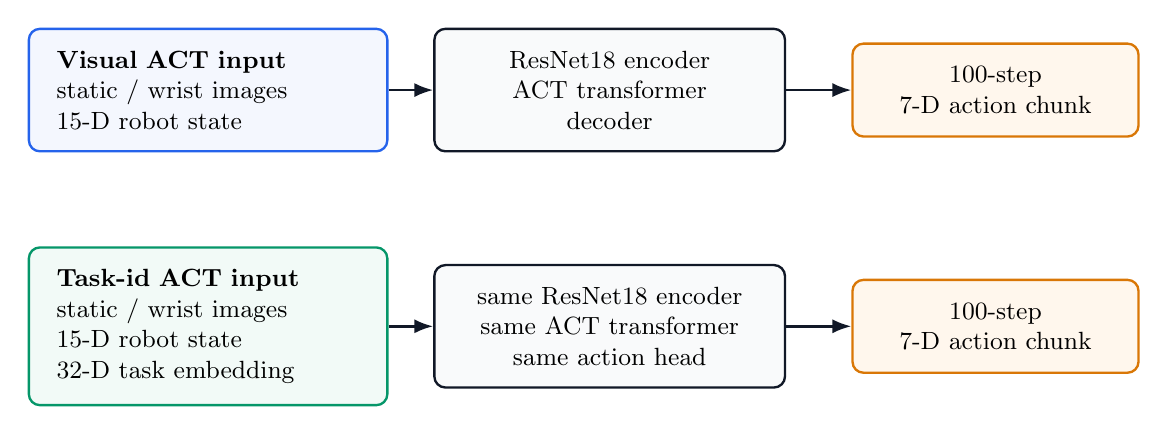
\begin{tikzpicture}[
  font=\small,
  panel/.style={rounded corners=4pt, draw=#1, fill=#1!5, line width=0.85pt, align=left, inner xsep=10pt, inner ysep=8pt, minimum width=4.25cm, minimum height=1.48cm, text width=3.85cm},
  model/.style={rounded corners=4pt, draw=ink, fill=softgray, line width=0.85pt, align=center, inner xsep=10pt, inner ysep=8pt, minimum width=4.15cm, minimum height=1.48cm, text width=3.75cm},
  output/.style={rounded corners=4pt, draw=evalorange, fill=softorange, line width=0.85pt, align=center, inner xsep=9pt, inner ysep=8pt, minimum width=3.35cm, minimum height=1.18cm, text width=3.0cm},
  arrow/.style={-{Latex[length=2.4mm]}, line width=0.9pt, draw=ink}
]
\node[panel=sourceblue] (vin) at (0,0.95) {\textbf{Visual ACT input}\\static / wrist images\\15-D robot state};
\node[model] (vact) at (5.1,0.95) {ResNet18 encoder\\ACT transformer\\decoder};
\node[output] (vout) at (10.0,0.95) {100-step\\7-D action chunk};

\node[panel=taskgreen] (tin) at (0,-2.05) {\textbf{Task-id ACT input}\\static / wrist images\\15-D robot state\\32-D task embedding};
\node[model] (tact) at (5.1,-2.05) {same ResNet18 encoder\\same ACT transformer\\same action head};
\node[output] (tout) at (10.0,-2.05) {100-step\\7-D action chunk};

\draw[arrow] (vin.east) -- (vact.west);
\draw[arrow] (vact.east) -- (vout.west);
\draw[arrow] (tin.east) -- (tact.west);
\draw[arrow] (tact.east) -- (tout.west);
\end{tikzpicture}}
\caption{Visual ACT 与 task-id ACT 的输入差异。task-id ACT 把语言任务映射为 32 维任务嵌入，并把它并入低维条件输入；视觉 backbone、ACT 主体和 7 维动作输出与视觉基线一致。}
\label{fig:task_id_arch}
\end{figure}

task-id 模型从对应 visual ACT checkpoint 继续训练。B-only task-id 从 B-only visual checkpoint 初始化，ABC-mixed task-id 从 ABC-mixed visual checkpoint 初始化；checkpoint 选择和训练步数在实验设置中给出。这种设计保留了视觉基线已经学到的低层动作和图像特征，再把任务目标写入低维条件输入。

\subsection{Action chunking 与重规划}

训练时的 chunk size 决定模型一次学习预测多长的未来动作，本实验固定为 100。闭环推理时，模型不一定执行完整 100 步动作后再看图像；$n_\text{action steps}$ 控制每次前向预测后实际执行多少步。$n=100$ 表示完整消费一个动作块，$n=20$ 表示执行前 20 步后重新观测当前图像并再次预测。

这一机制和 D 环境闭环结果直接相关。较大的 $n$ 保留 ACT 学到的长动作连续性，但接触点或方向一旦偏离，后续动作仍会沿着旧轨迹继续执行；较小的 $n$ 增加反馈频率，让策略更早看到抽屉是否被拉开、滑块是否移动、方块是否偏离。实验中我们保持训练 chunk size 不变，只改变推理阶段的 $n_\text{action steps}$，避免把模型容量变化和闭环控制频率混在一起。

\section{实验设置与诊断}

\subsection{训练设置}

四个模型共享图像预处理、ACT 主体结构和动作输出定义。输入图像来自静态相机和 wrist camera，统一缩放到 $256\times256$；动作维度为 7，训练时每个样本提供 100 步动作块和对应 padding mask。visual ACT 使用 15 维机器人状态；task-id ACT 在同一状态旁加入 32 维任务嵌入，内部条件向量变为 47 维。训练/验证按 episode 划分，验证比例为 0.05，task-id fine-tune 复用各自 visual baseline 的随机种子和 split，避免 checkpoint 选择受到验证集变化影响。

\begin{table}[!htbp]
\centering
\small
\caption{主要训练超参数。两组源环境对照和两组 task-id fine-tune 使用相同优化设置；task-id 行只改变低维条件输入。}
\label{tab:training_hparams_v2}
\begin{tabularx}{\linewidth}{@{}l>{\raggedright\arraybackslash}X@{}}
\toprule
项目 & 设置 \\
\midrule
Network architecture & LeRobot ACT；ResNet18 visual encoder；transformer hidden dim 512；dropout 0.1；7-D action head \\
Image inputs & \texttt{observation.images.image}, \texttt{observation.images.wrist\_image}; resolution $256\times256$ \\
State / task condition & visual ACT: 15-D robot state; task-id ACT: 15-D state + 32-D task embedding = 47-D condition \\
Action chunking & training chunk size $K=100$; default inference $n_\text{action steps}=100$ \\
Batch / split & batch size 16; episode-level validation fraction 0.05; seed 20260531 \\
Optimizer & AdamW; learning rate $1\times10^{-5}$ for policy and backbone; weight decay $1\times10^{-4}$ \\
Loss & Action L1 with KL regularization; $\lambda_{\mathrm{KL}}=10$ \\
Stability settings & gradient clipping 10; AMP off; validation interval 5000 steps \\
\bottomrule
\end{tabularx}
\end{table}

训练日志保留了每 5000 步的验证结果。图~\ref{fig:training_validation_curves} 展示四个模型的 validation \actionlone{}：visual baseline 在 50k 步内持续下降；task-id fine-tune 从已有视觉 checkpoint 接着优化，B-only 在 90k 步附近达到最低验证误差，ABC-mixed 在 95k 步达到最低验证误差。图~\ref{fig:training_taskid_curves} 进一步给出 task-id 阶段的 train/validation 曲线，验证误差没有在后段反弹，后续 D 环境评估均使用这些 best-validation checkpoint。

\begin{figure}[!htbp]
\centering
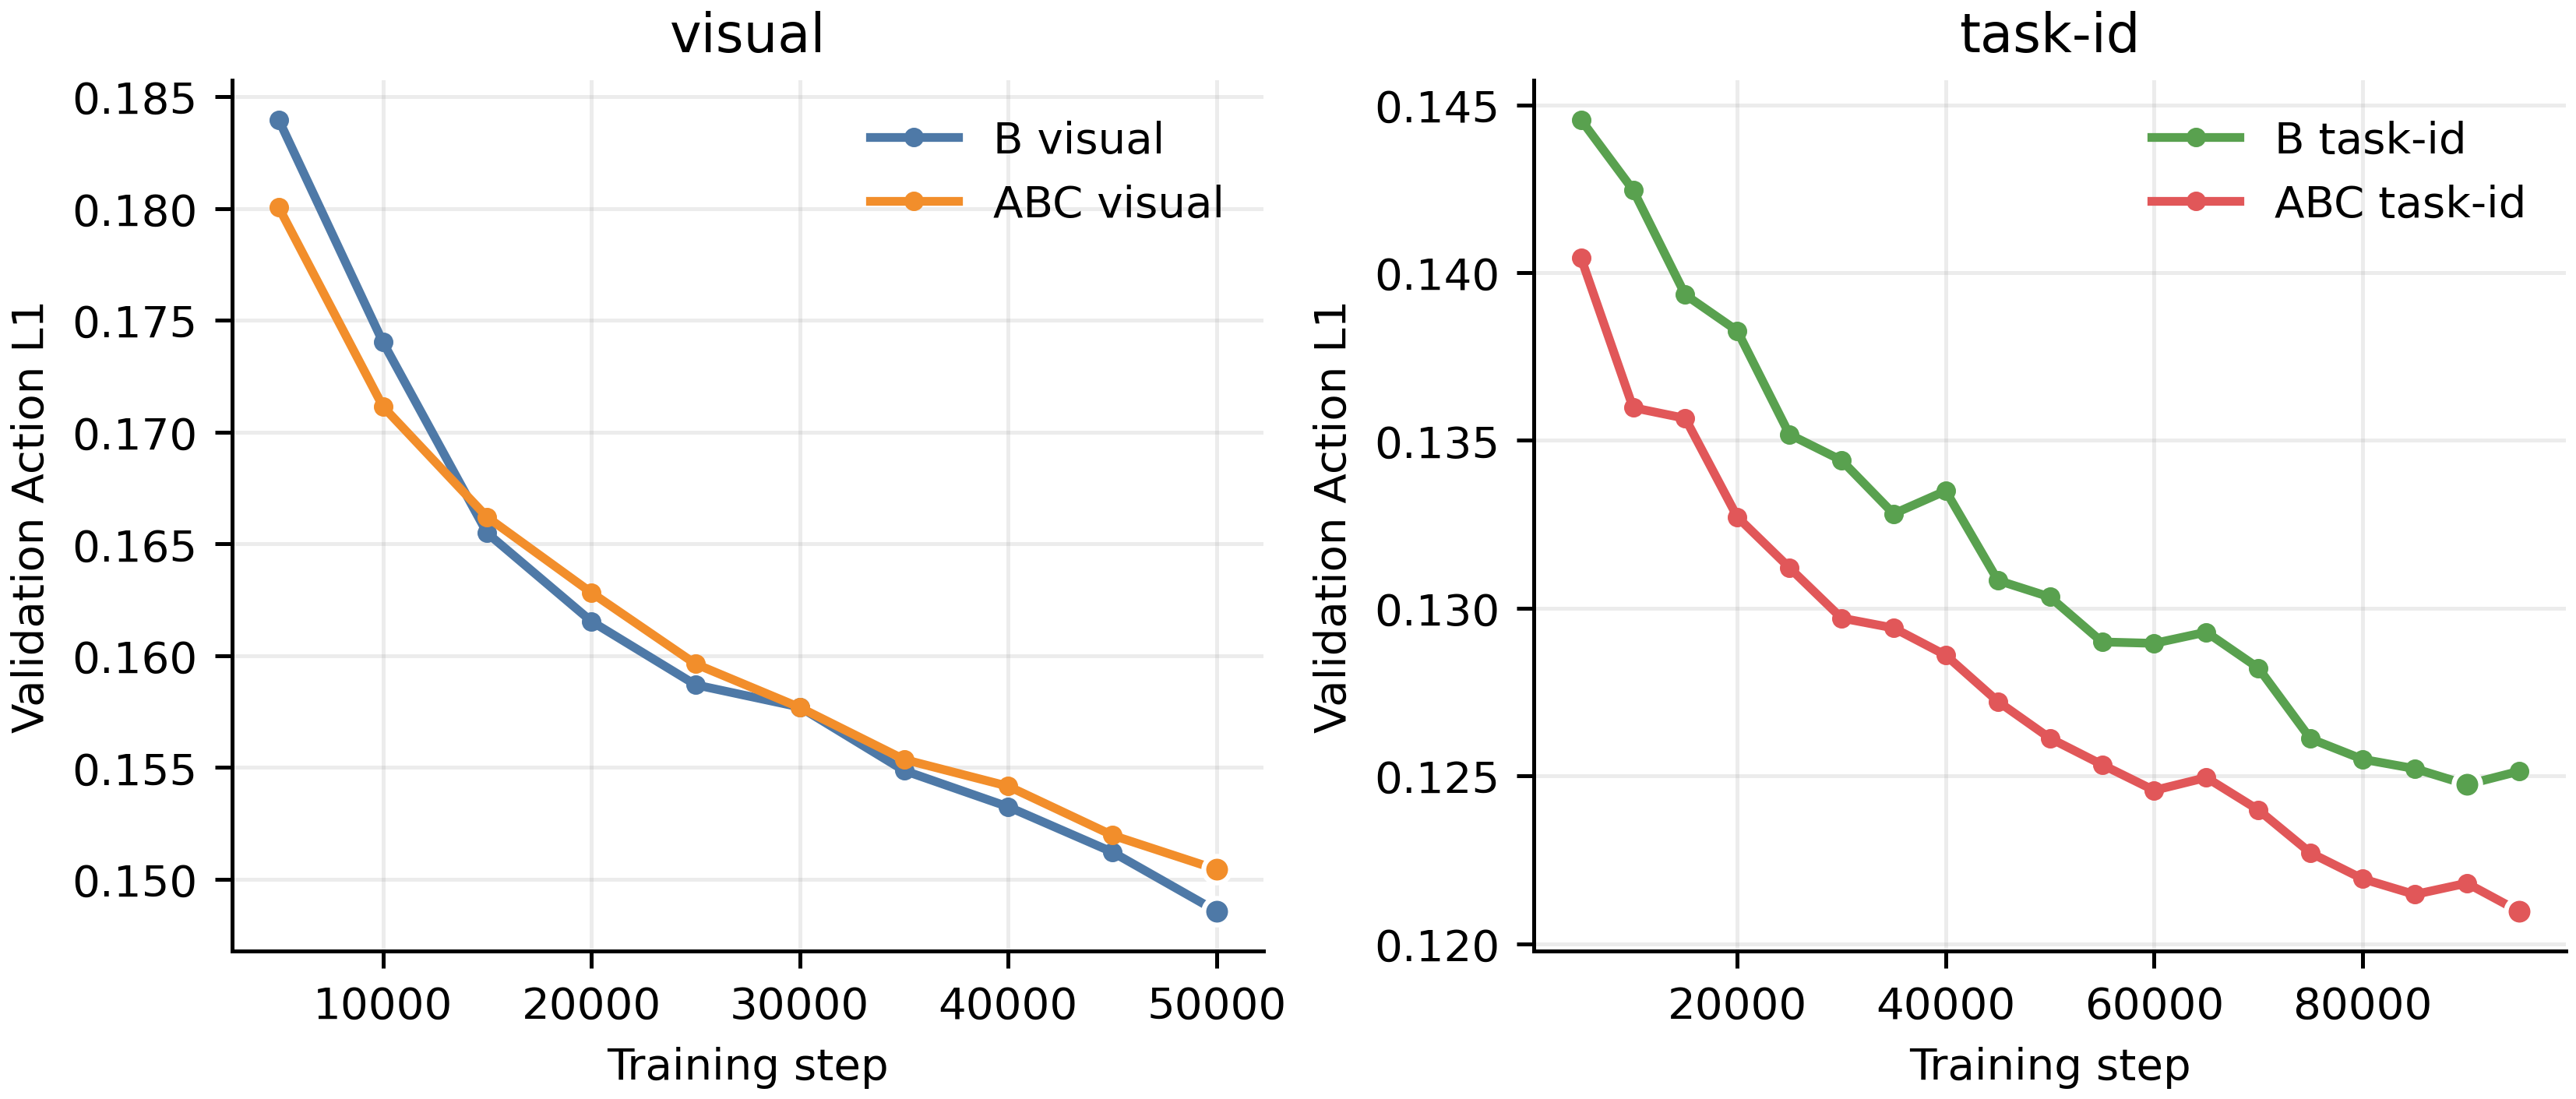
\includegraphics[width=0.94\linewidth]{../results/figures/step4/training_validation_action_l1_curves.png}
\caption{四个主模型的 source validation \actionlone{} 曲线。左图为 visual ACT baseline，右图为从 visual checkpoint 初始化后的 task-id fine-tune。}
\label{fig:training_validation_curves}
\end{figure}

\begin{figure}[!htbp]
\centering
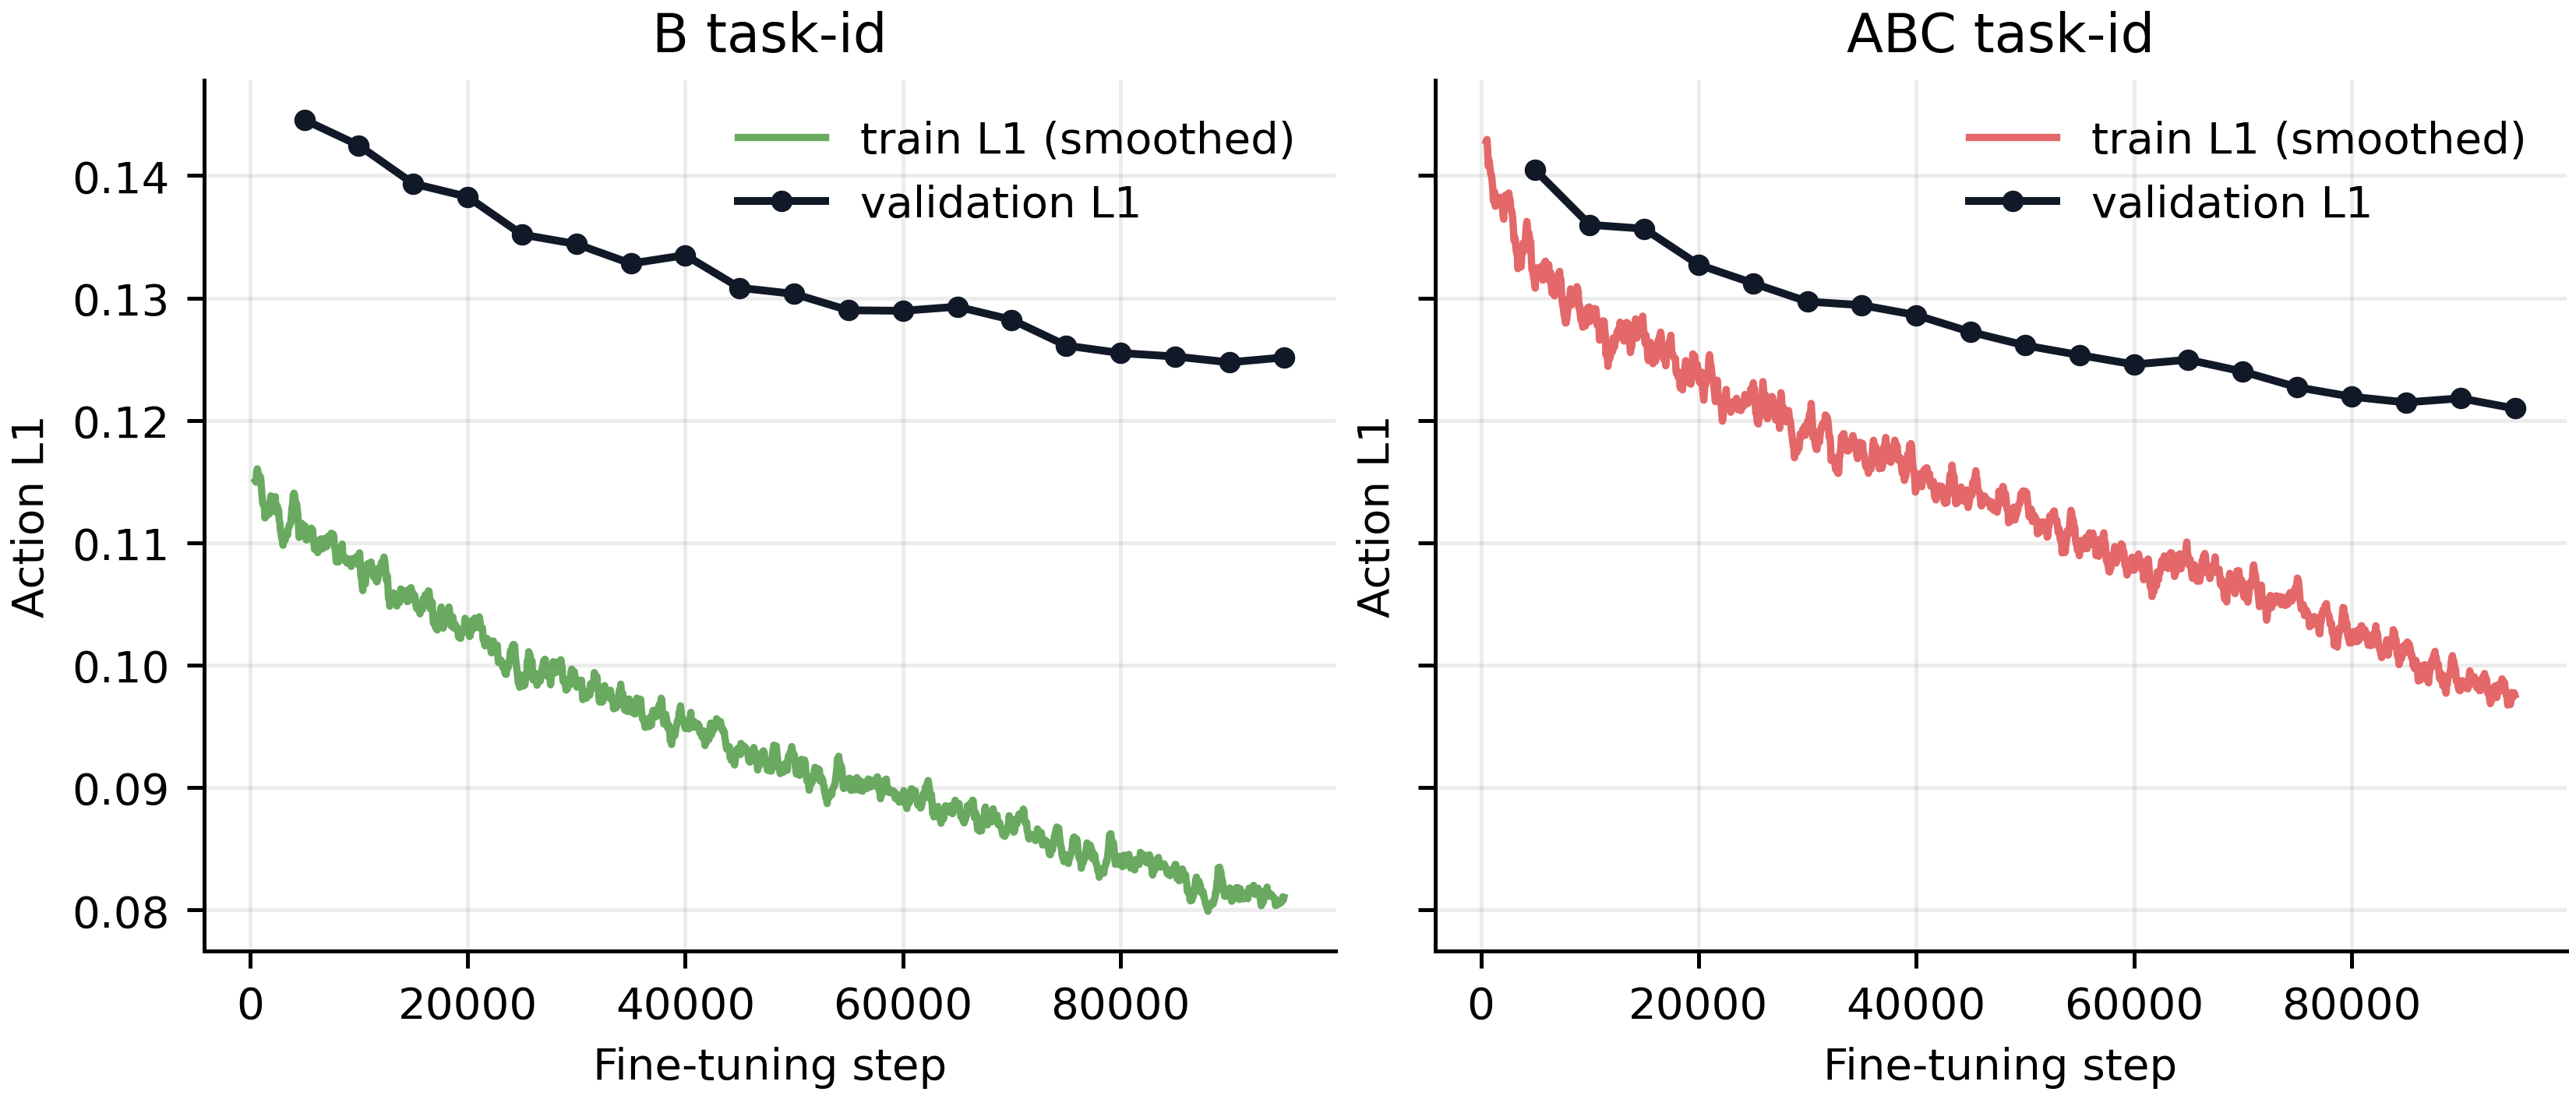
\includegraphics[width=0.94\linewidth]{../results/figures/step4/training_taskid_train_val_action_l1.png}
\caption{task-id fine-tune 阶段的 train/validation \actionlone{}。训练曲线用滑动平均显示，黑色点线为每次验证结果。}
\label{fig:training_taskid_curves}
\end{figure}

\begin{table}[!htbp]
\centering
\small
\caption{用于 D 环境评估的 checkpoint。task-id 模型从对应 visual checkpoint 初始化，按源环境验证集上的 best validation \actionlone{} 选择。}
\label{tab:checkpoint_selection_v2}
\begin{tabular}{llrrr}
\toprule
模型 & 训练源 & state dim & selected step & source val \actionlone{} \\
\midrule
B-only visual ACT & B & 15 & 50000 & 0.1486 \\
ABC-mixed visual ACT & A/B/C & 15 & 50000 & 0.1504 \\
B-only task-id ACT & B & 47 & 90000 & 0.1247 \\
ABC-mixed task-id ACT & A/B/C & 47 & 95000 & \best{0.1210} \\
\bottomrule
\end{tabular}
\end{table}

\FloatBarrier

\subsection{评估协议与指标}

D 环境离线评估在专家轨迹上运行，模型根据当前观测预测动作块，再与专家动作计算 L1。报告中同时给出 normalized \actionlone{} 和 raw \actionlone{}：前者在训练集 action normalization 空间里计算，便于跨 checkpoint 比较；后者回到原始动作尺度，能辅助判断误差落在哪些动作维度。

闭环 rollout 让策略在 CALVIN simulator 的 D 环境中执行动作。每条 evaluation sequence 包含 5 个子任务；Avg 表示平均完成子任务数，SR@k 表示至少连续完成 $k$ 个子任务的序列比例。该指标比离线 \actionlone{} 更受接触误差、动作块执行长度、重规划频率和 simulator 初始状态影响，因此后续结果同时展示动作误差和闭环执行。

\subsection{Horizon 诊断}

早期闭环测试使用 5 条 D 环境序列、B-only task-id checkpoint 和相同 inference bridge。每个子任务只执行 120 步时，五条序列的成功子任务数全为 0；把执行窗口改为 360 步后，成功向量变为 $[0,1,0,2,0]$。数值变化把问题定位到评估窗口：部分抽屉和方块任务需要更长接触过程，120 步会把晚出现的成功截断。

\begin{table}[!htbp]
\centering
\small
\caption{同一 B-only task-id checkpoint 的 horizon 诊断。两行使用同样 5 条 D 环境序列和同一套 simulator bridge。}
\label{tab:horizon_diag_v2}
\begin{tabularx}{0.88\linewidth}{@{}lXccc@{}}
\toprule
设置 & 5 条序列成功子任务数 & Avg & SR@1 & SR@2 \\
\midrule
120 steps & $[0,0,0,0,0]$ & 0.00 & 0.00 & 0.00 \\
360 steps & $[0,1,0,2,0]$ & \best{0.60} & \best{0.40} & \best{0.20} \\
\bottomrule
\end{tabularx}
\end{table}

\begin{figure}[!htbp]
\centering
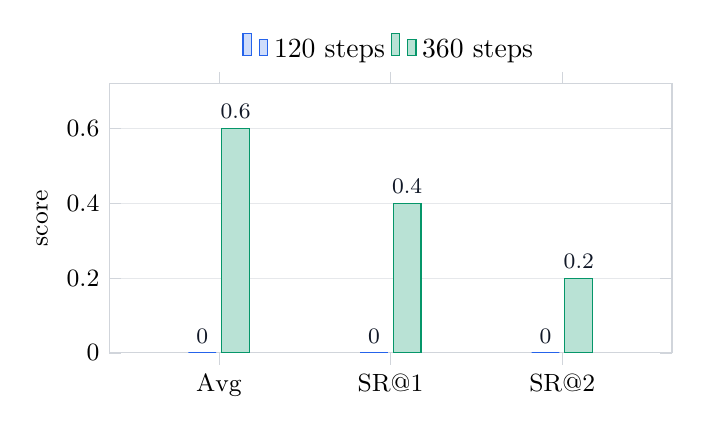
\begin{tikzpicture}
\begin{axis}[
  width=0.72\linewidth,
  height=5.0cm,
  ybar,
  bar width=10pt,
  ymin=0,
  ymax=0.72,
  symbolic x coords={Avg,SR@1,SR@2},
  xtick=data,
  ylabel={score},
  enlarge x limits=0.32,
  legend style={draw=none, fill=none, at={(0.5,1.04)}, anchor=south, legend columns=2},
  axis line style={draw=linegray},
  tick style={draw=linegray},
  ymajorgrids=true,
  grid style={draw=linegray!55},
  nodes near coords,
  every node near coord/.append style={font=\footnotesize, text=ink},
  tick label style={font=\small},
  label style={font=\small}
]
\addplot+[draw=sourceblue, fill=sourceblue!22] coordinates {(Avg,0.00) (SR@1,0.00) (SR@2,0.00)};
\addplot+[draw=taskgreen, fill=taskgreen!28] coordinates {(Avg,0.60) (SR@1,0.40) (SR@2,0.20)};
\legend{120 steps, 360 steps}
\end{axis}
\end{tikzpicture}
\caption{120 步与 360 步执行窗口的闭环诊断。执行窗口变长后，平均完成子任务数和 chain success rate 同时从零恢复。}
\label{fig:horizon_diag_v2}
\end{figure}

正式的 50 条 D 环境 rollout 全部采用 360 步窗口；action chunking 消融只改变 $n_\text{action steps}$，保留相同 horizon，用同一执行窗口比较 ACT 的重规划频率。

\section{实验结果与现象分析}

\subsection{D 环境离线动作误差}

D 环境离线 \actionlone{} 衡量策略在未见过的专家轨迹附近预测动作的精度。表~\ref{tab:d_action_l1_v2} 给出四个 checkpoint 的完整结果。ABC-mixed visual ACT 的 normalized \actionlone{} 为 0.5657，低于 B-only visual ACT 的 0.6498；加入 task-id 后，两者差距扩大到 0.1037。任务条件输入也带来稳定收益：B-only 下降 0.0446，ABC-mixed 下降 0.0642。

\begin{table}[!htbp]
\centering
\small
\caption{D 环境离线 \actionlone{}。Normalized 指训练归一化动作空间中的误差，Raw 指原始动作尺度下的误差；数值越低越好。}
\label{tab:d_action_l1_v2}
\begin{tabular}{lcc}
\toprule
模型 & normalized \actionlone{} $\downarrow$ & raw \actionlone{} $\downarrow$ \\
\midrule
B-only visual ACT & 0.6498 & 0.2097 \\
ABC-mixed visual ACT & 0.5657 & 0.1682 \\
B-only task-id ACT & 0.6052 & 0.1888 \\
ABC-mixed task-id ACT & \best{0.5016} & \best{0.1446} \\
\bottomrule
\end{tabular}
\end{table}

\begin{figure}[!htbp]
\centering
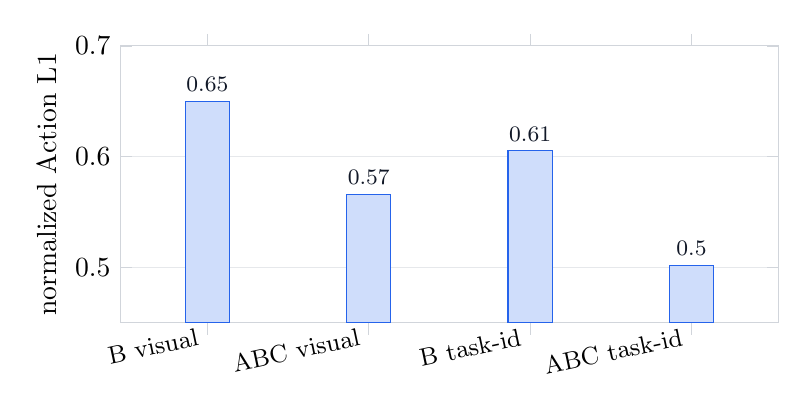
\begin{tikzpicture}
\begin{axis}[
  width=0.82\linewidth,
  height=5.1cm,
  ybar,
  bar width=16pt,
  ymin=0.45,
  ymax=0.70,
  symbolic x coords={B visual,ABC visual,B task-id,ABC task-id},
  xtick=data,
  ylabel={normalized Action L1},
  xticklabel style={font=\small, rotate=12, anchor=east},
  ymajorgrids=true,
  grid style={draw=linegray!55},
  axis line style={draw=linegray},
  tick style={draw=linegray},
  point meta=y,
  nodes near coords={\pgfmathprintnumber[fixed,precision=2]{\pgfplotspointmeta}},
  every node near coord/.append style={font=\footnotesize, text=ink},
  enlarge x limits=0.18,
]
\addplot+[draw=sourceblue, fill=sourceblue!22] coordinates {
  (B visual,0.6498)
  (ABC visual,0.5657)
  (B task-id,0.6052)
  (ABC task-id,0.5016)
};
\end{axis}
\end{tikzpicture}
\caption{D 环境 normalized \actionlone{} 对比。多源环境训练和 task-id 条件输入的收益可以叠加，ABC-mixed task-id 得到最低动作误差。}
\label{fig:d_action_l1_v2}
\end{figure}

两类改动对应两种误差来源。A/B/C 混合训练带来更多桌面外观和物体状态变化，减小源环境到 D 环境的视觉偏移；task-id embedding 把语言任务写入低维条件，减少同一桌面状态下目标不明造成的动作平均化。离线误差只在专家轨迹附近比较动作，闭环实验继续检查误差积累后的执行表现。

episode-level 配对统计检查平均值是否由少数 easy episode 拉动。图~\ref{fig:episode_paired_gain} 使用 6135 个 D 环境 episode，对同一 episode 上两个模型的 normalized \actionlone{} 做差。ABC-mixed visual 相对 B-only visual 的 win rate 为 78.9\%，median reduction 为 0.081；ABC-mixed task-id 相对 ABC-mixed visual 的 win rate 为 75.0\%，median reduction 为 0.057；ABC-mixed task-id 相对 B-only visual 的 win rate 达到 87.8\%，median reduction 为 0.145。分布主体都在零线以上，平均提升来自大多数 episode 的稳定移动。

\begin{figure}[!htbp]
\centering
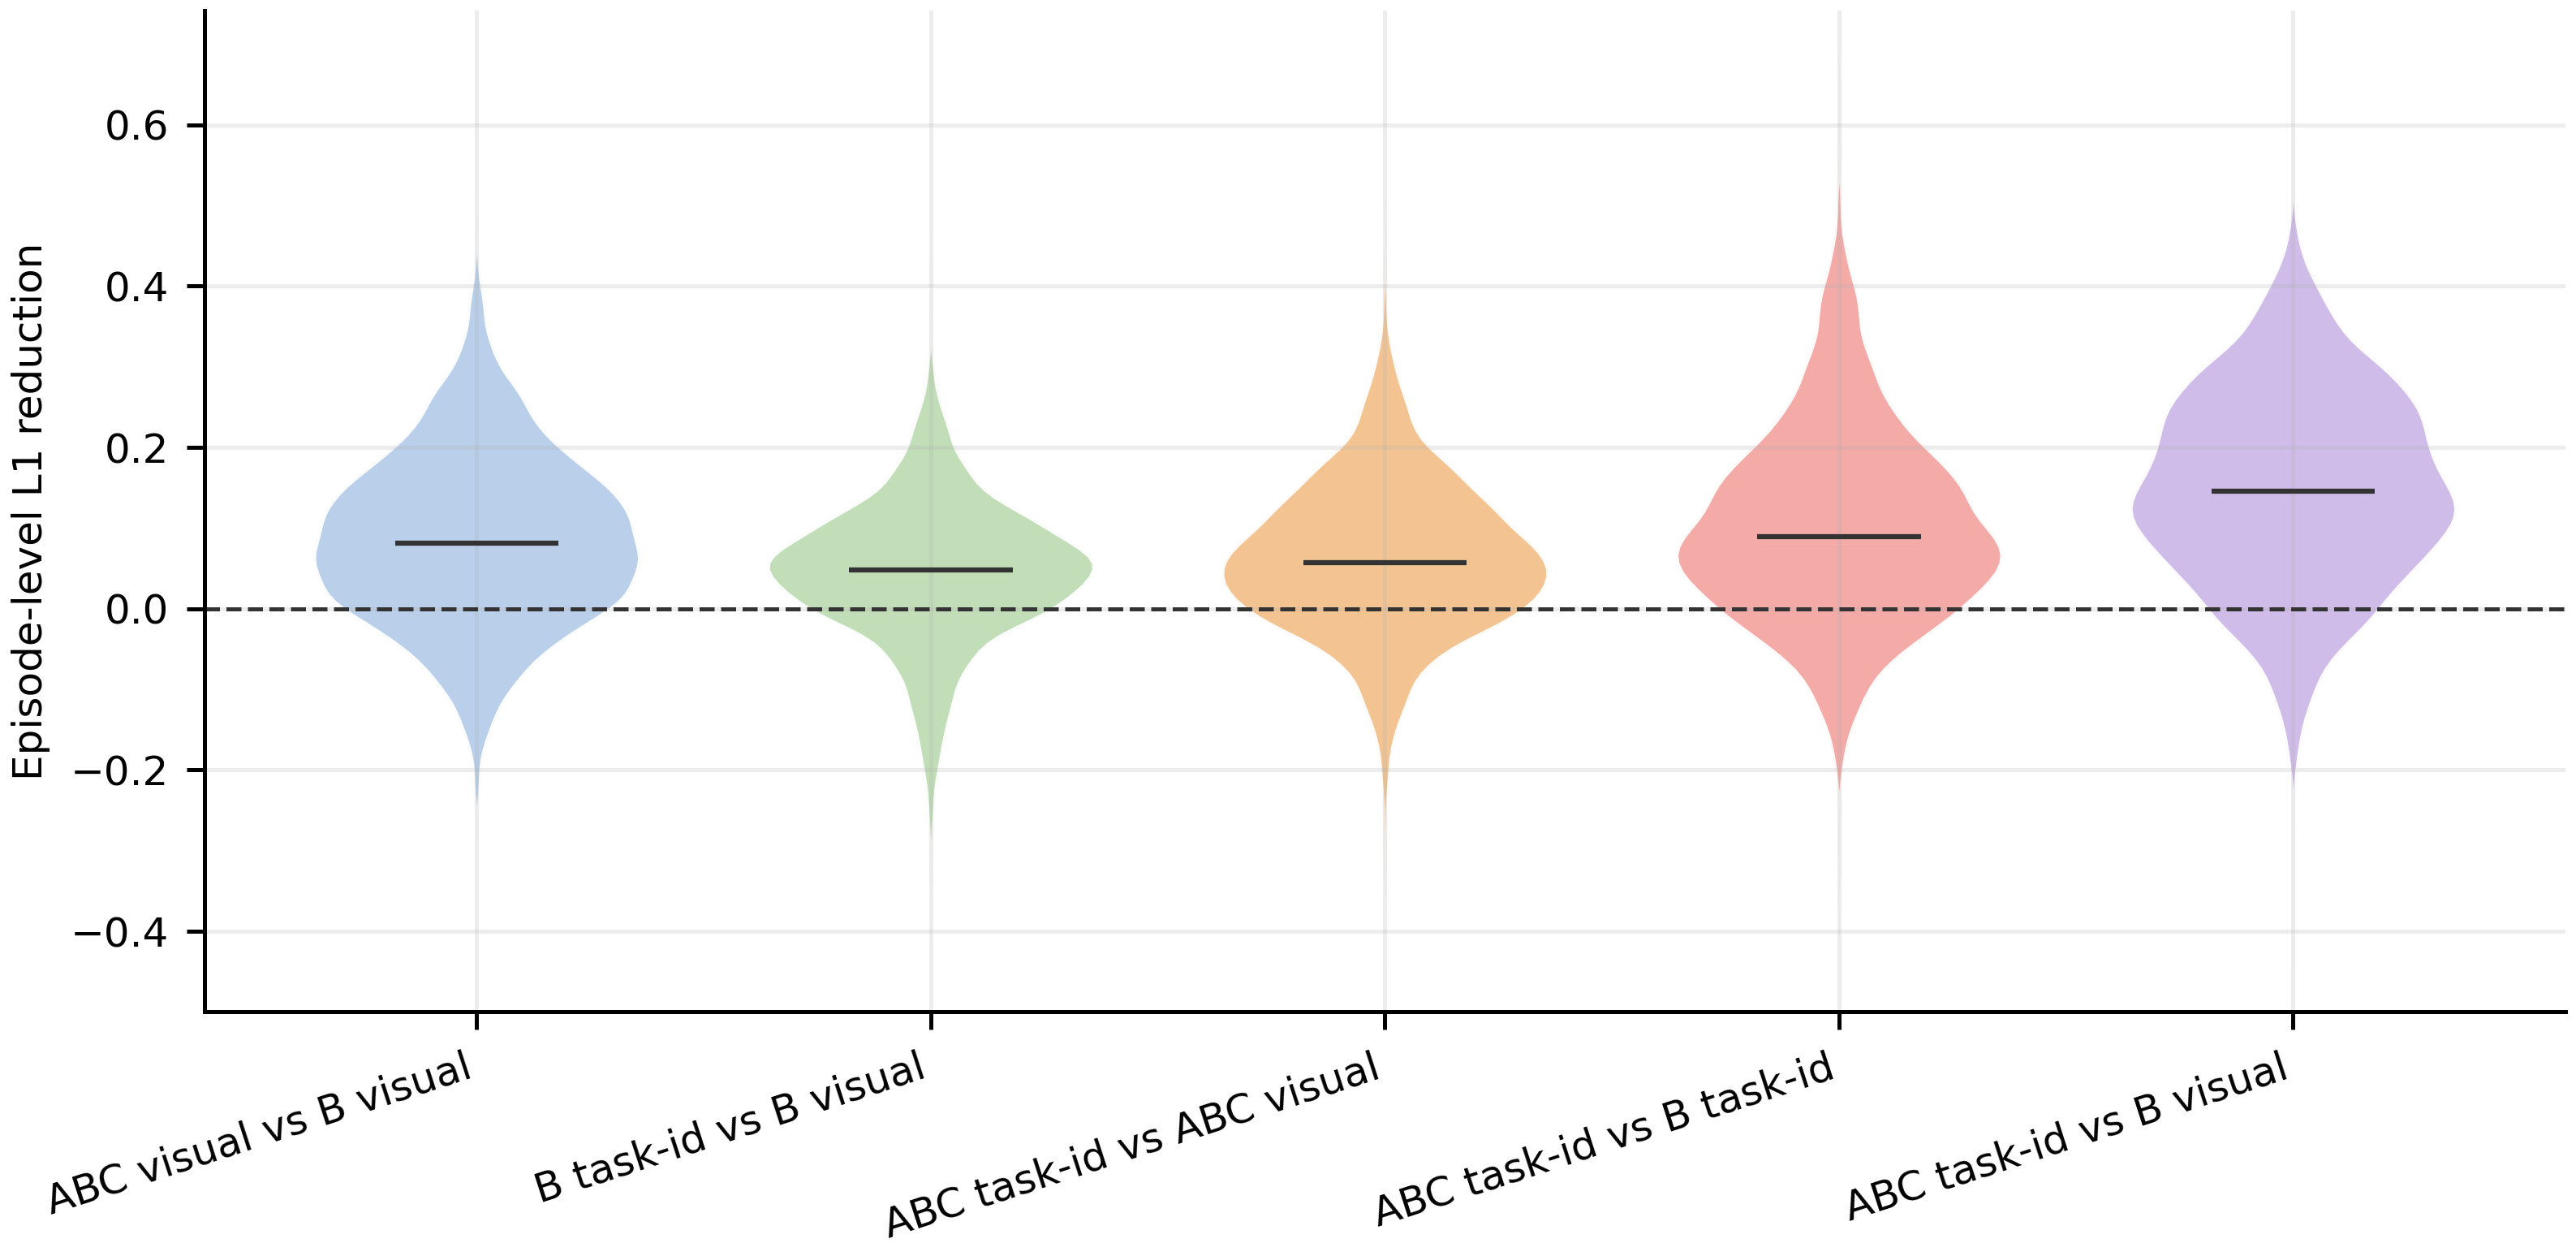
\includegraphics[width=0.92\linewidth]{../figures/track2_extra/extra1024_episode_paired_improvement_violin.png}
\caption{D 环境 episode-level 配对 \actionlone{} reduction 分布。每个 violin 对应同一批 6135 个 episode；零线以上表示横轴标签左侧模型在该 episode 上误差更低。}
\label{fig:episode_paired_gain}
\end{figure}

\subsection{视觉偏移与离线扰动评估}

Visual Distribution Shift 指训练源环境和目标 D 环境之间的图像统计与接触线索变化。这里的变化包括亮度差异、桌面纹理、相机视角中物体位置、抽屉和滑块状态、wrist camera 看到的末端接触区域。图~\ref{fig:vds_stats} 给出源环境与 D 环境的 metadata 统计距离：B-only 源环境到 D 环境的 image mean L2 距离在静态相机和 wrist camera 上分别为 0.258 和 0.285；ABC-mixed 对应距离降到 0.027 和 0.018。多源训练让视觉输入分布更接近 D 环境，这与表~\ref{tab:d_action_l1_v2} 中 ABC visual 更低的 D 环境 \actionlone{} 相互印证。

\begin{figure}[!htbp]
\centering
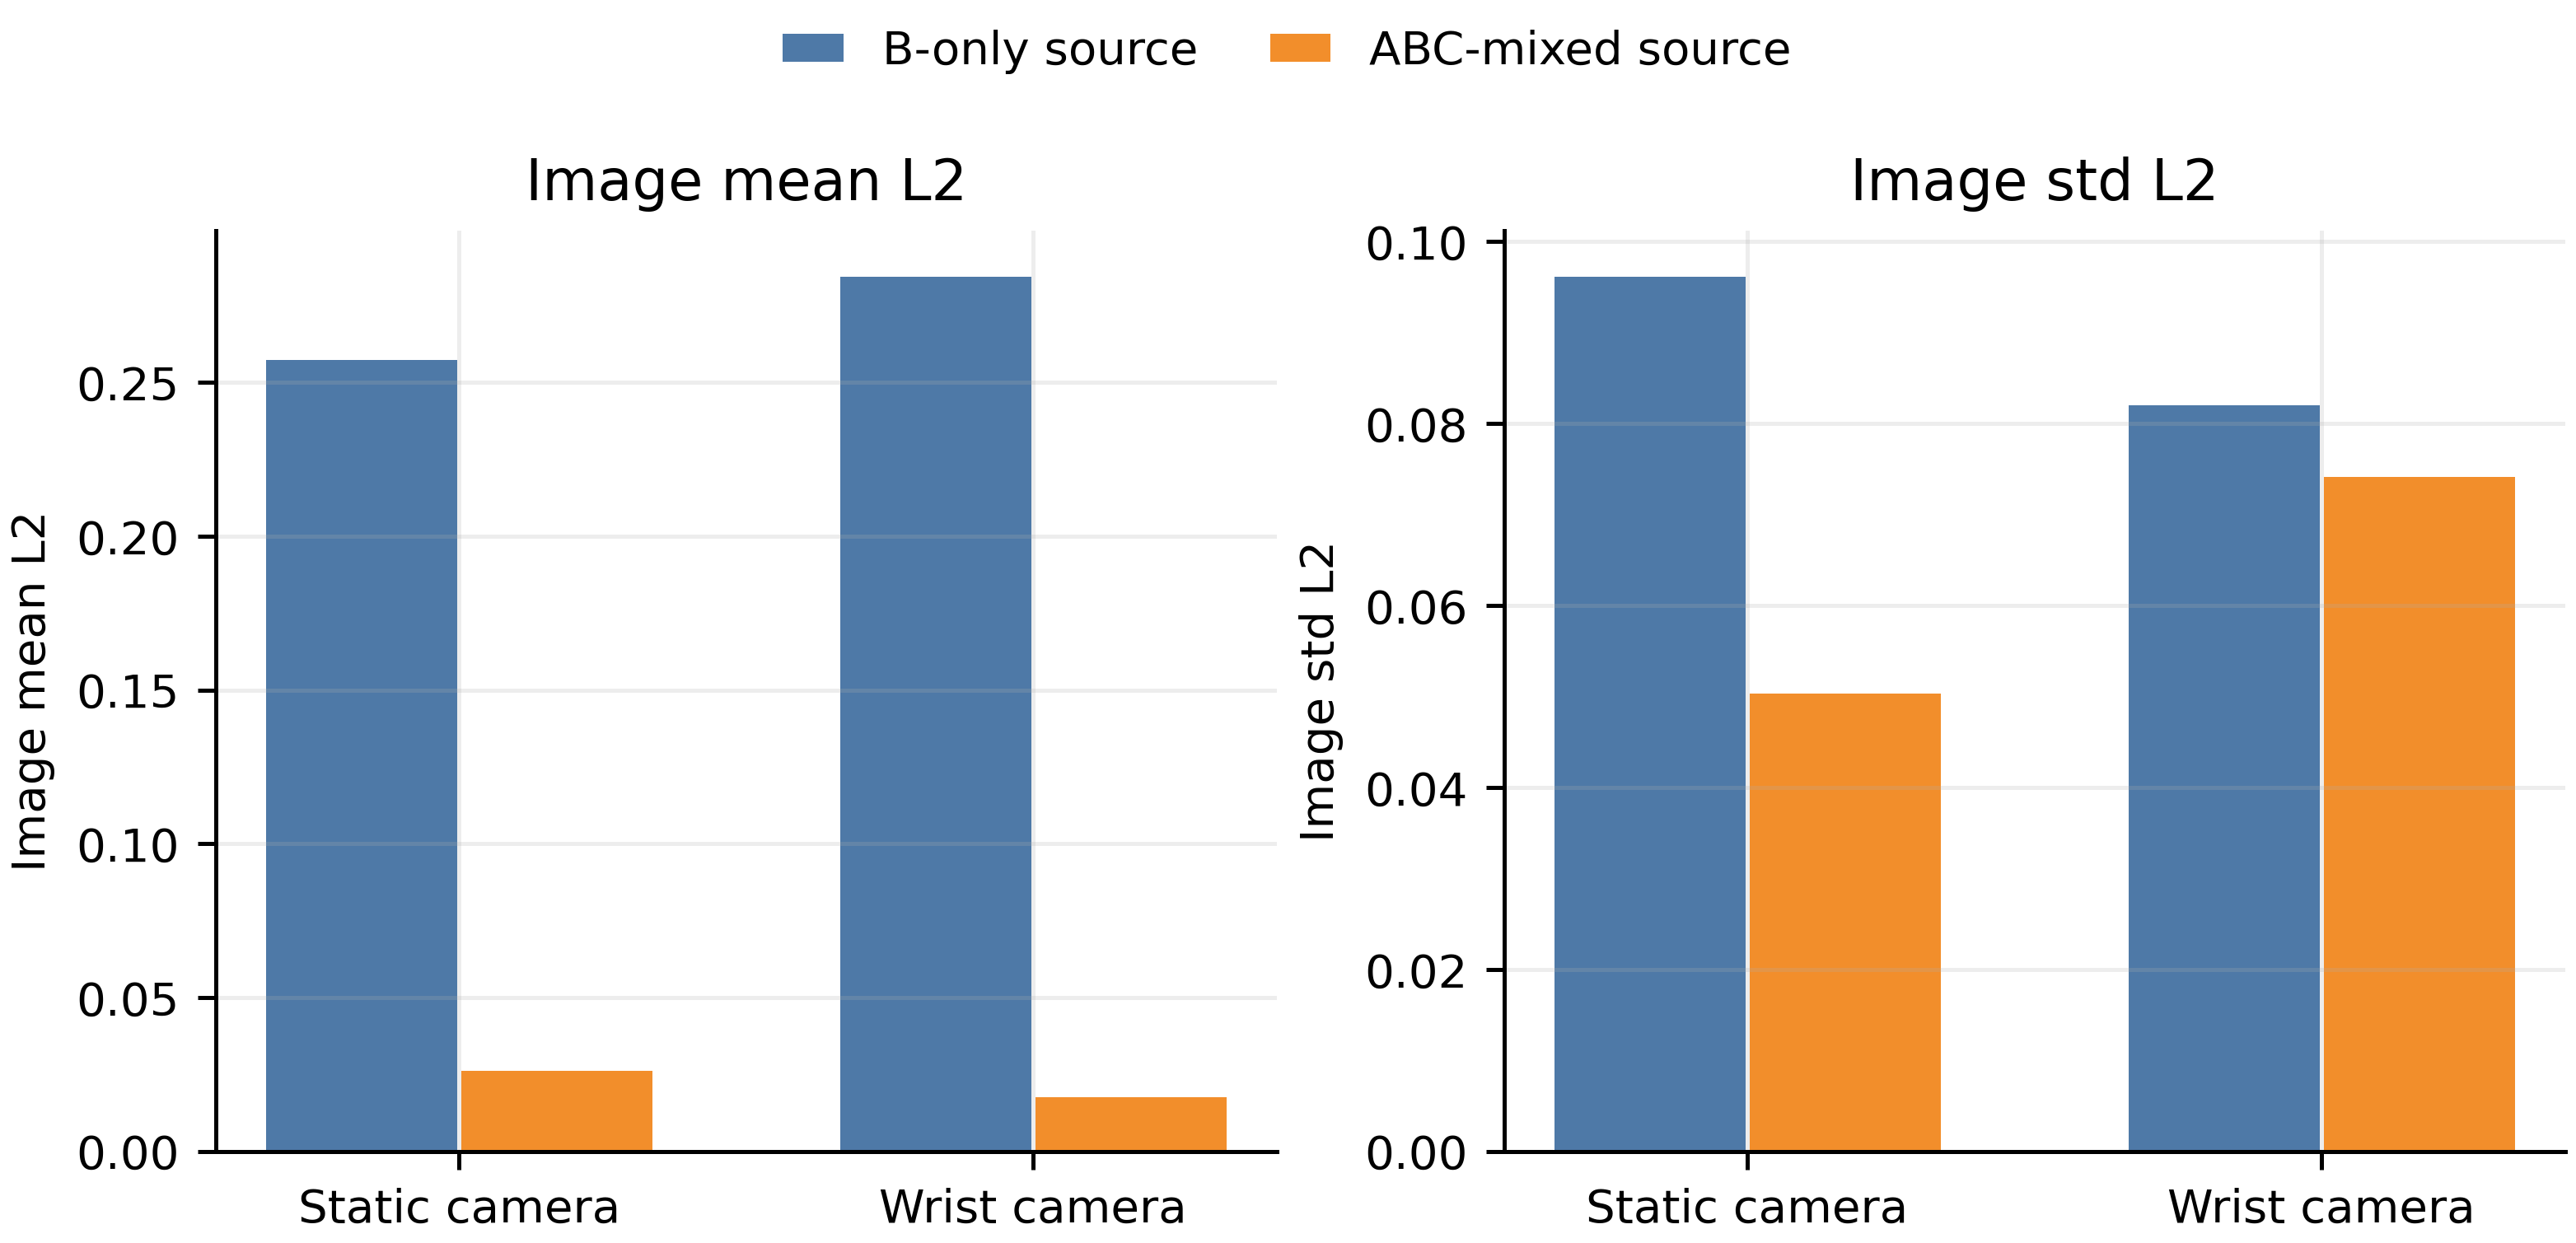
\includegraphics[width=0.82\linewidth]{../results/figures/step4/visual_distribution_shift_stats.png}
\caption{训练源环境与 D 环境的图像统计距离。ABC-mixed 源环境在静态相机和 wrist camera 上都更接近 D 环境。}
\label{fig:vds_stats}
\end{figure}

按 task family 聚合 clean 条件下的 D-1024 \actionlone{} 后，ABC-mixed visual 在所有 family 上低于 B-only visual。图~\ref{fig:visual_family_l1} 中，差距最大的 family 为 rotate、slider 和 push，分别降低 0.130、0.129 和 0.120；drawer 的差距最小，只有 0.016。每行括号给出该 family 在 D-1024 子集中的 episode 数，避免把少量样本的波动误读为稳定结论。

\begin{figure}[!htbp]
\centering
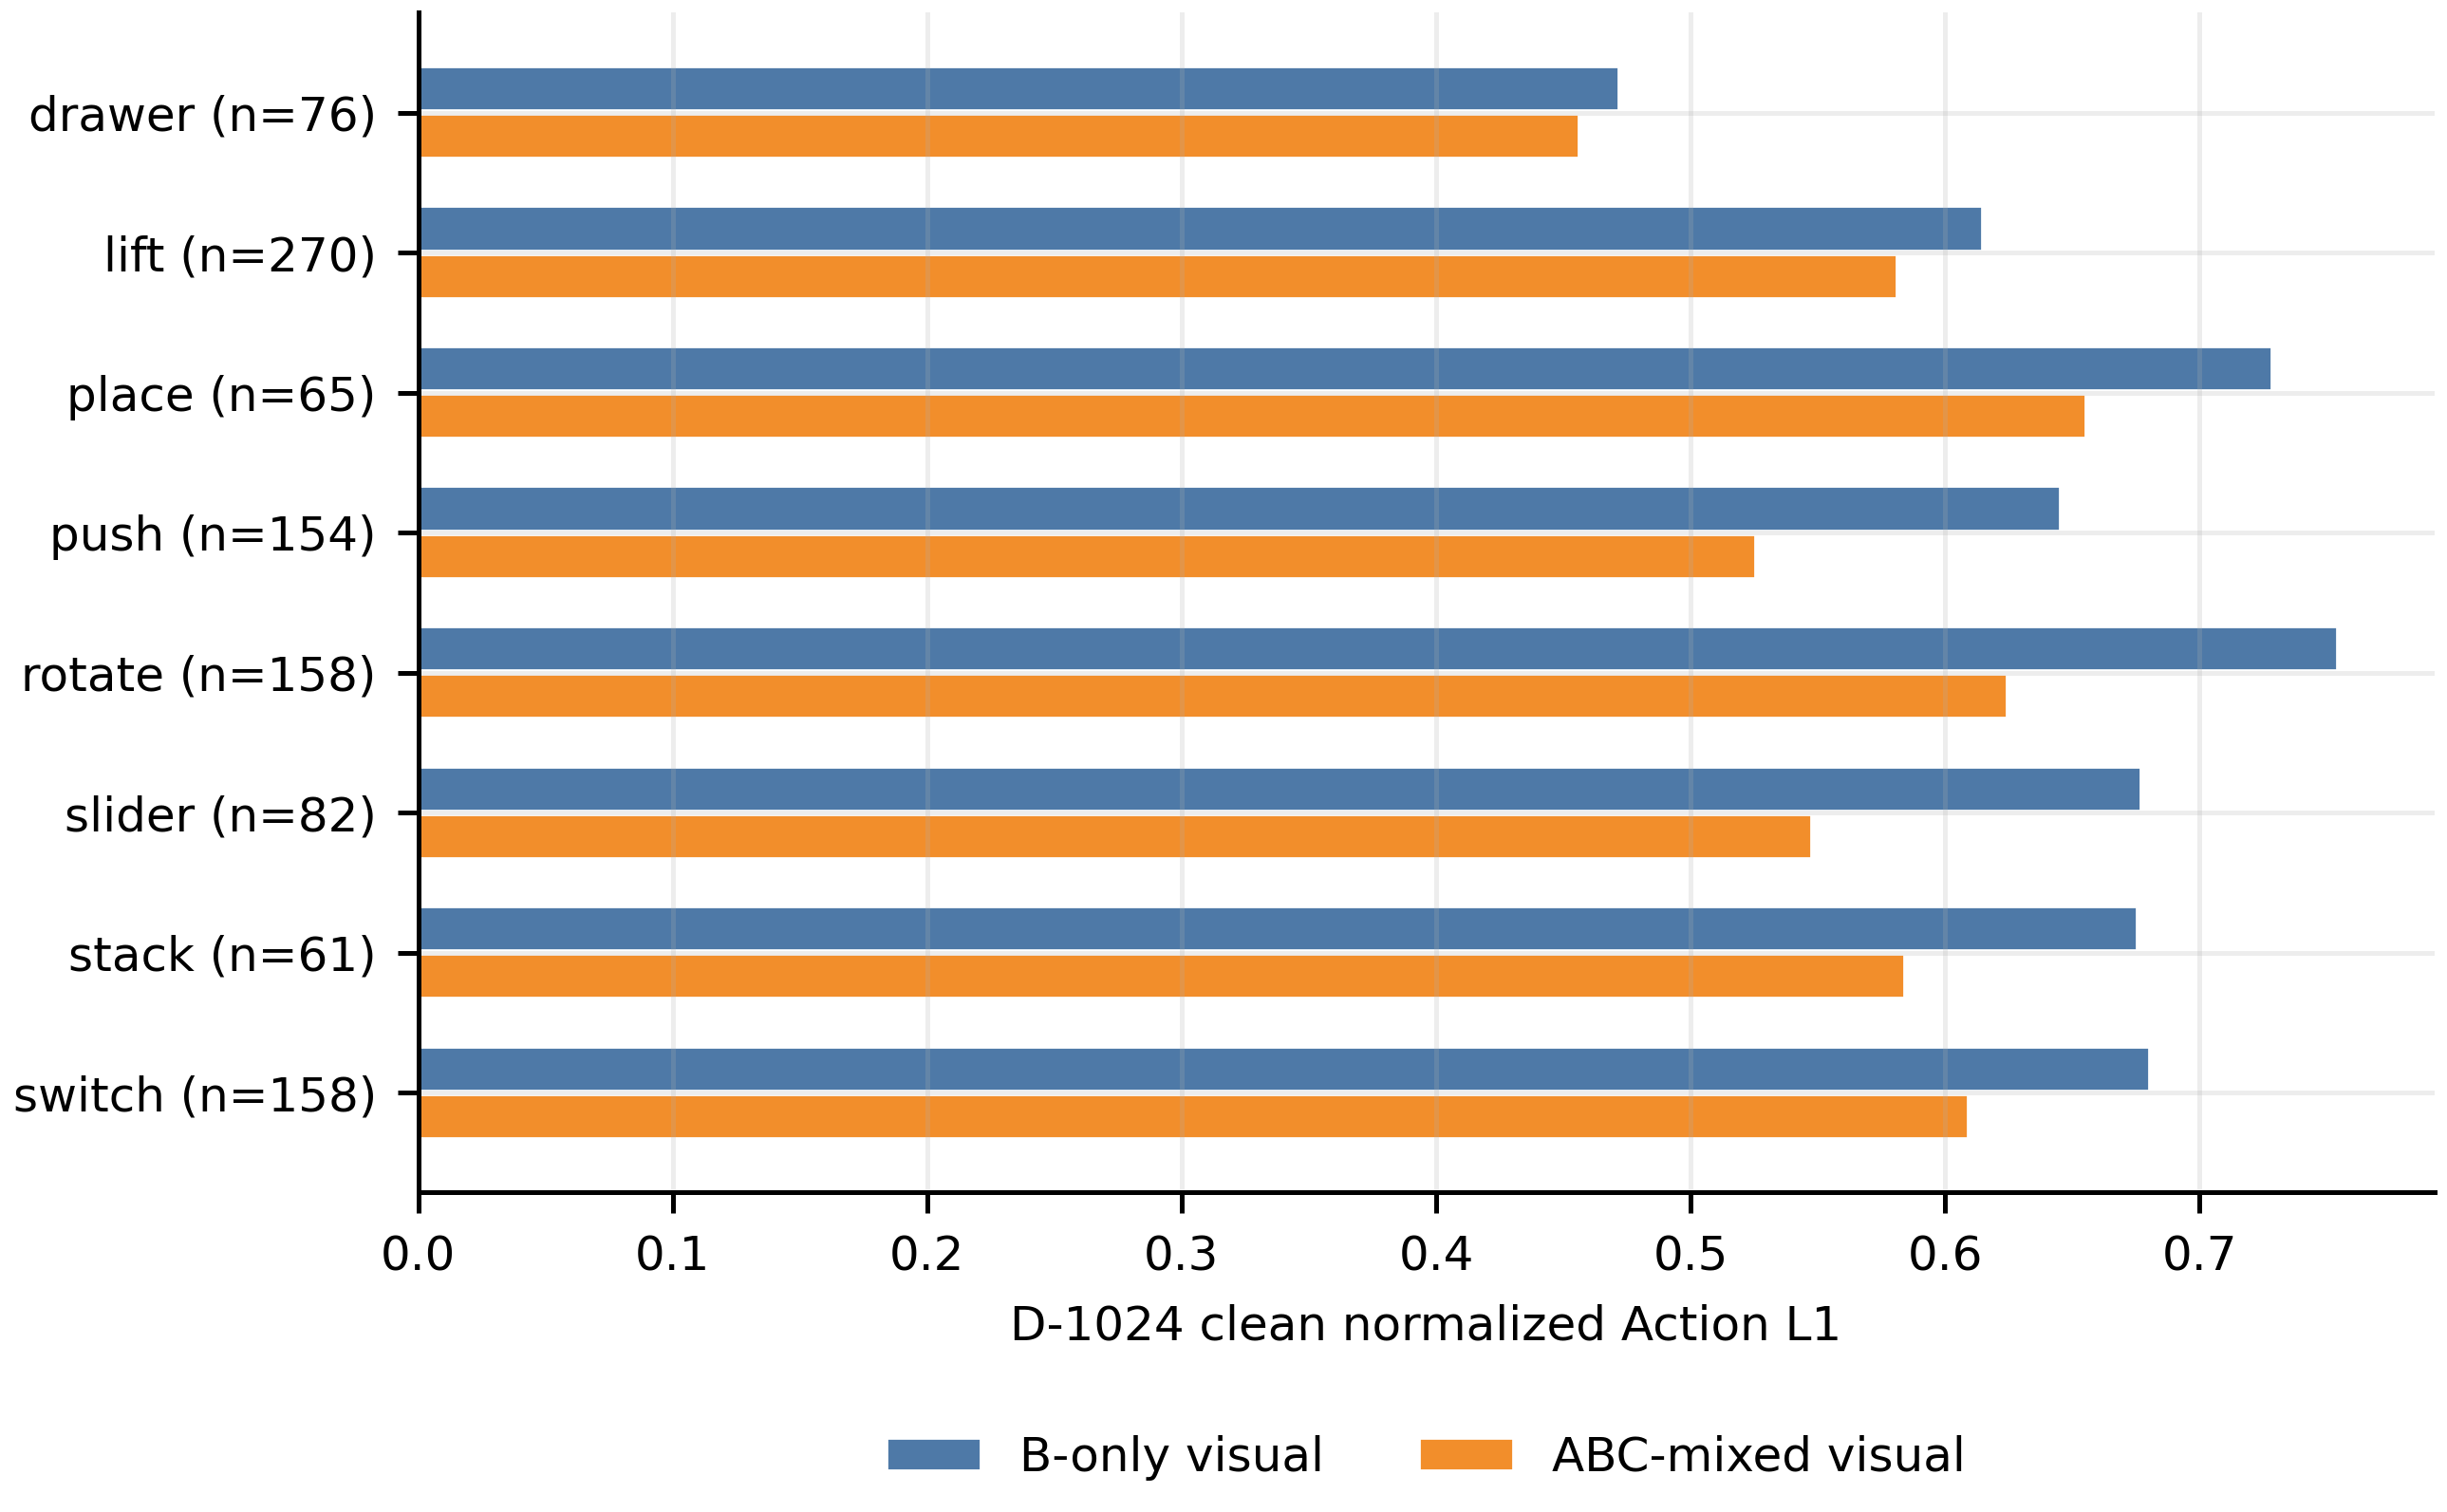
\includegraphics[width=0.84\linewidth]{../figures/track2_extra/extra1024_visual_task_family_clean_l1.png}
\caption{D-1024 clean 条件下按 task family 聚合的 normalized \actionlone{}。横轴越小越好；括号中为 episode count。}
\label{fig:visual_family_l1}
\end{figure}

为把视觉偏移拆开，我们在同一批 D-1024 offline 样本上构造 8 个观测条件：clean、暗光、亮光、模糊、噪声、静态相机 gray-out、wrist camera gray-out、双相机 gray-out。图~\ref{fig:visual_shift_contact_sheet} 显示这些扰动直接作用在模型输入图像上，动作标签和机器人状态保持不变。该评估覆盖 1024 episodes、62000 frames；每个条件都用同一批 episode 做配对统计。

\begin{figure}[!htbp]
\centering
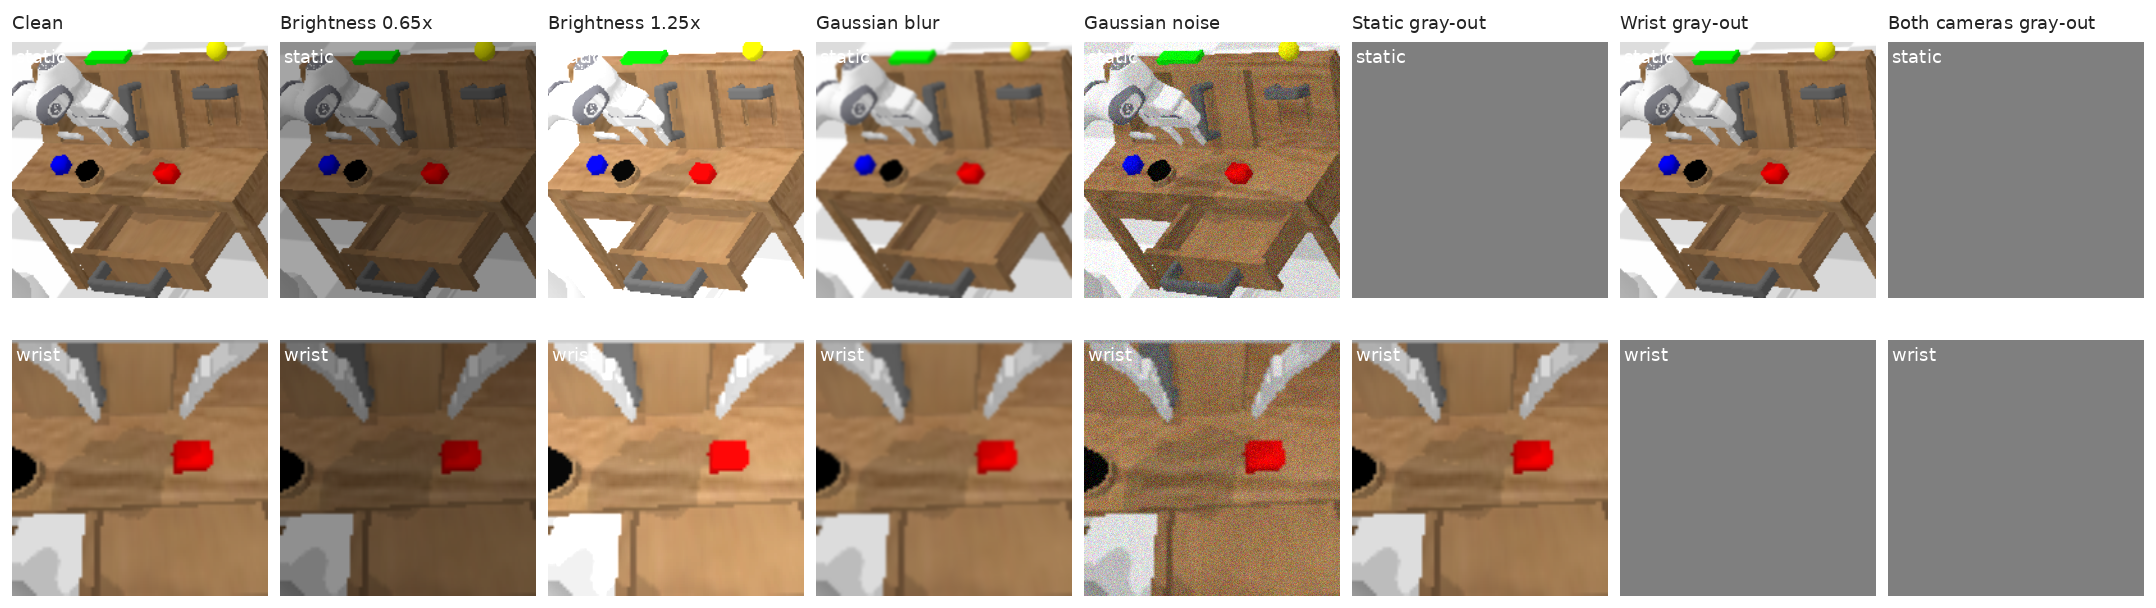
\includegraphics[width=0.98\linewidth]{../figures/track2_extra/extra1024_visual_full_robustness_visual_shift_contact_sheet.png}
\caption{D-1024 offline 视觉扰动示例。上排为静态相机，下排为 wrist camera；扰动只改变图像输入。}
\label{fig:visual_shift_contact_sheet}
\end{figure}

\begin{table}[!htbp]
\centering
\footnotesize
\caption{D-1024 offline 视觉扰动结果。括号内为相对 clean 的 normalized \actionlone{} 绝对增量和相对退化；Win 表示同一 episode 上 ABC-mixed visual 误差低于 B-only visual 的比例。}
\label{tab:visual_shift_1024}
\begin{tabularx}{\linewidth}{lXXX}
\toprule
条件 & B-only visual & ABC-mixed visual & ABC Win \\
\midrule
Clean & 0.654 (-- / --) & \best{0.574} (-- / --) & 77.2\% \\
Dark & 0.657 (+0.003 / 0.4\%) & \best{0.578} (+0.003 / 0.6\%) & 79.0\% \\
Bright & 0.666 (+0.012 / 1.8\%) & \best{0.584} (+0.010 / 1.7\%) & 80.1\% \\
Blur & 0.662 (+0.008 / 1.3\%) & \best{0.581} (+0.007 / 1.1\%) & 78.4\% \\
Noise & 0.676 (+0.022 / 3.4\%) & \best{0.600} (+0.026 / 4.5\%) & 78.7\% \\
Static gray & 0.625 (-0.030 / -4.5\%) & \best{0.587} (+0.013 / 2.3\%) & 70.3\% \\
Wrist gray & 0.688 (+0.034 / 5.1\%) & \best{0.667} (+0.092 / 16.1\%) & 61.9\% \\
Both gray & 0.703 (+0.049 / 7.4\%) & \best{0.664} (+0.090 / 15.6\%) & 75.2\% \\
\bottomrule
\end{tabularx}
\end{table}

Static gray 是表~\ref{tab:visual_shift_1024} 中最需要单独读的一行。B-only visual 在 clean 条件下的 normalized \actionlone{} 为 0.654，遮掉静态相机后降到 0.625，这是全部扰动条件里唯一的大幅负增量；ABC-mixed visual 在同一扰动下从 0.574 升到 0.587，方向相反。我们为这个反常结果做了额外检查：100-episode 复核中，B-only visual 同样从 0.645 降到 0.610；输入断言和 16 个随机样例确认，static gray 只把 static image 替换为 [0,1] 图像空间中的 0.5 灰度，wrist image、robot state、action label 与 task 字段都没有变化。这个现象更像 B-only visual 依赖了静态相机里的 B 环境背景伪线索，遮掉 static view 后减少了这类误导；ABC-mixed visual 见过 A/B/C 多个背景，更倾向于使用真实的视觉状态，因此遮掉 static view 后出现轻微退化。这个结果只作为诊断证据，不表示 gray-out 可以作为提升策略。

表~\ref{tab:visual_shift_1024} 中，ABC-mixed visual 在 8 个条件下都保持更低 \actionlone{}。clean 条件的配对差值为 -0.0837，95\% bootstrap CI 为 [-0.0903, -0.0773]；wrist gray 后差值缩小到 -0.0261，CI 为 [-0.0310, -0.0211]。这组数值把 ABC-mixed 的收益和风险同时摆出来：多源视觉覆盖降低了整体动作误差，wrist camera 被遮挡时优势被压缩，近端接触线索在 ABC-mixed visual 中承担了更大权重。

\begin{figure}[!htbp]
\centering
\begin{minipage}[t]{0.49\linewidth}
\centering
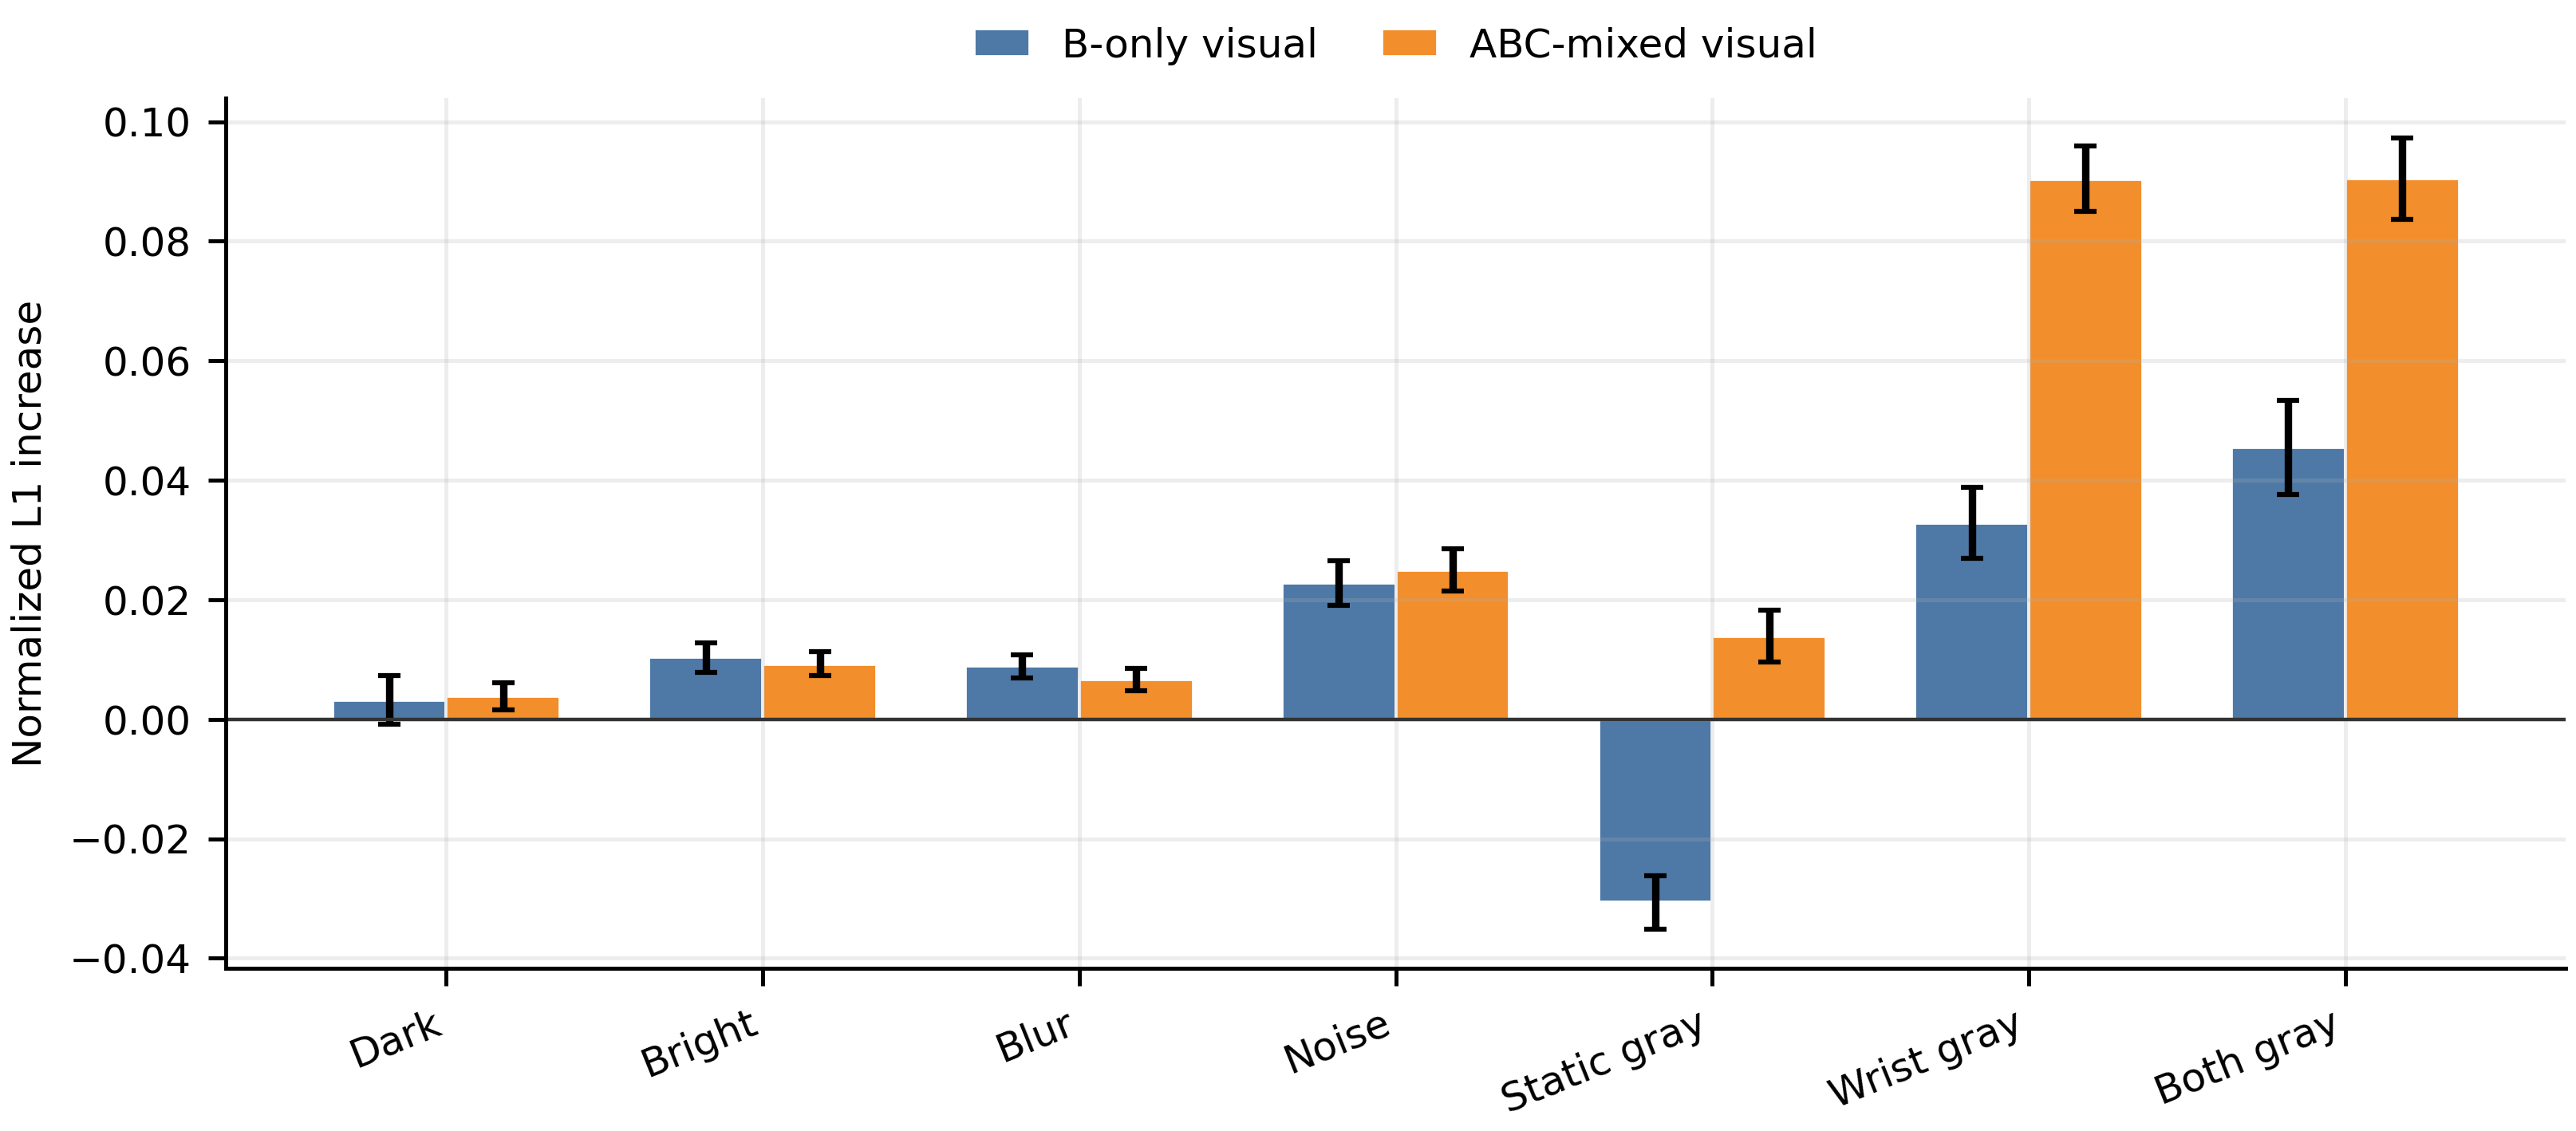
\includegraphics[width=\linewidth]{../figures/track2_extra/extra1024_visual_full_robustness_visual_degradation_ci.png}
\end{minipage}
\hfill
\begin{minipage}[t]{0.49\linewidth}
\centering
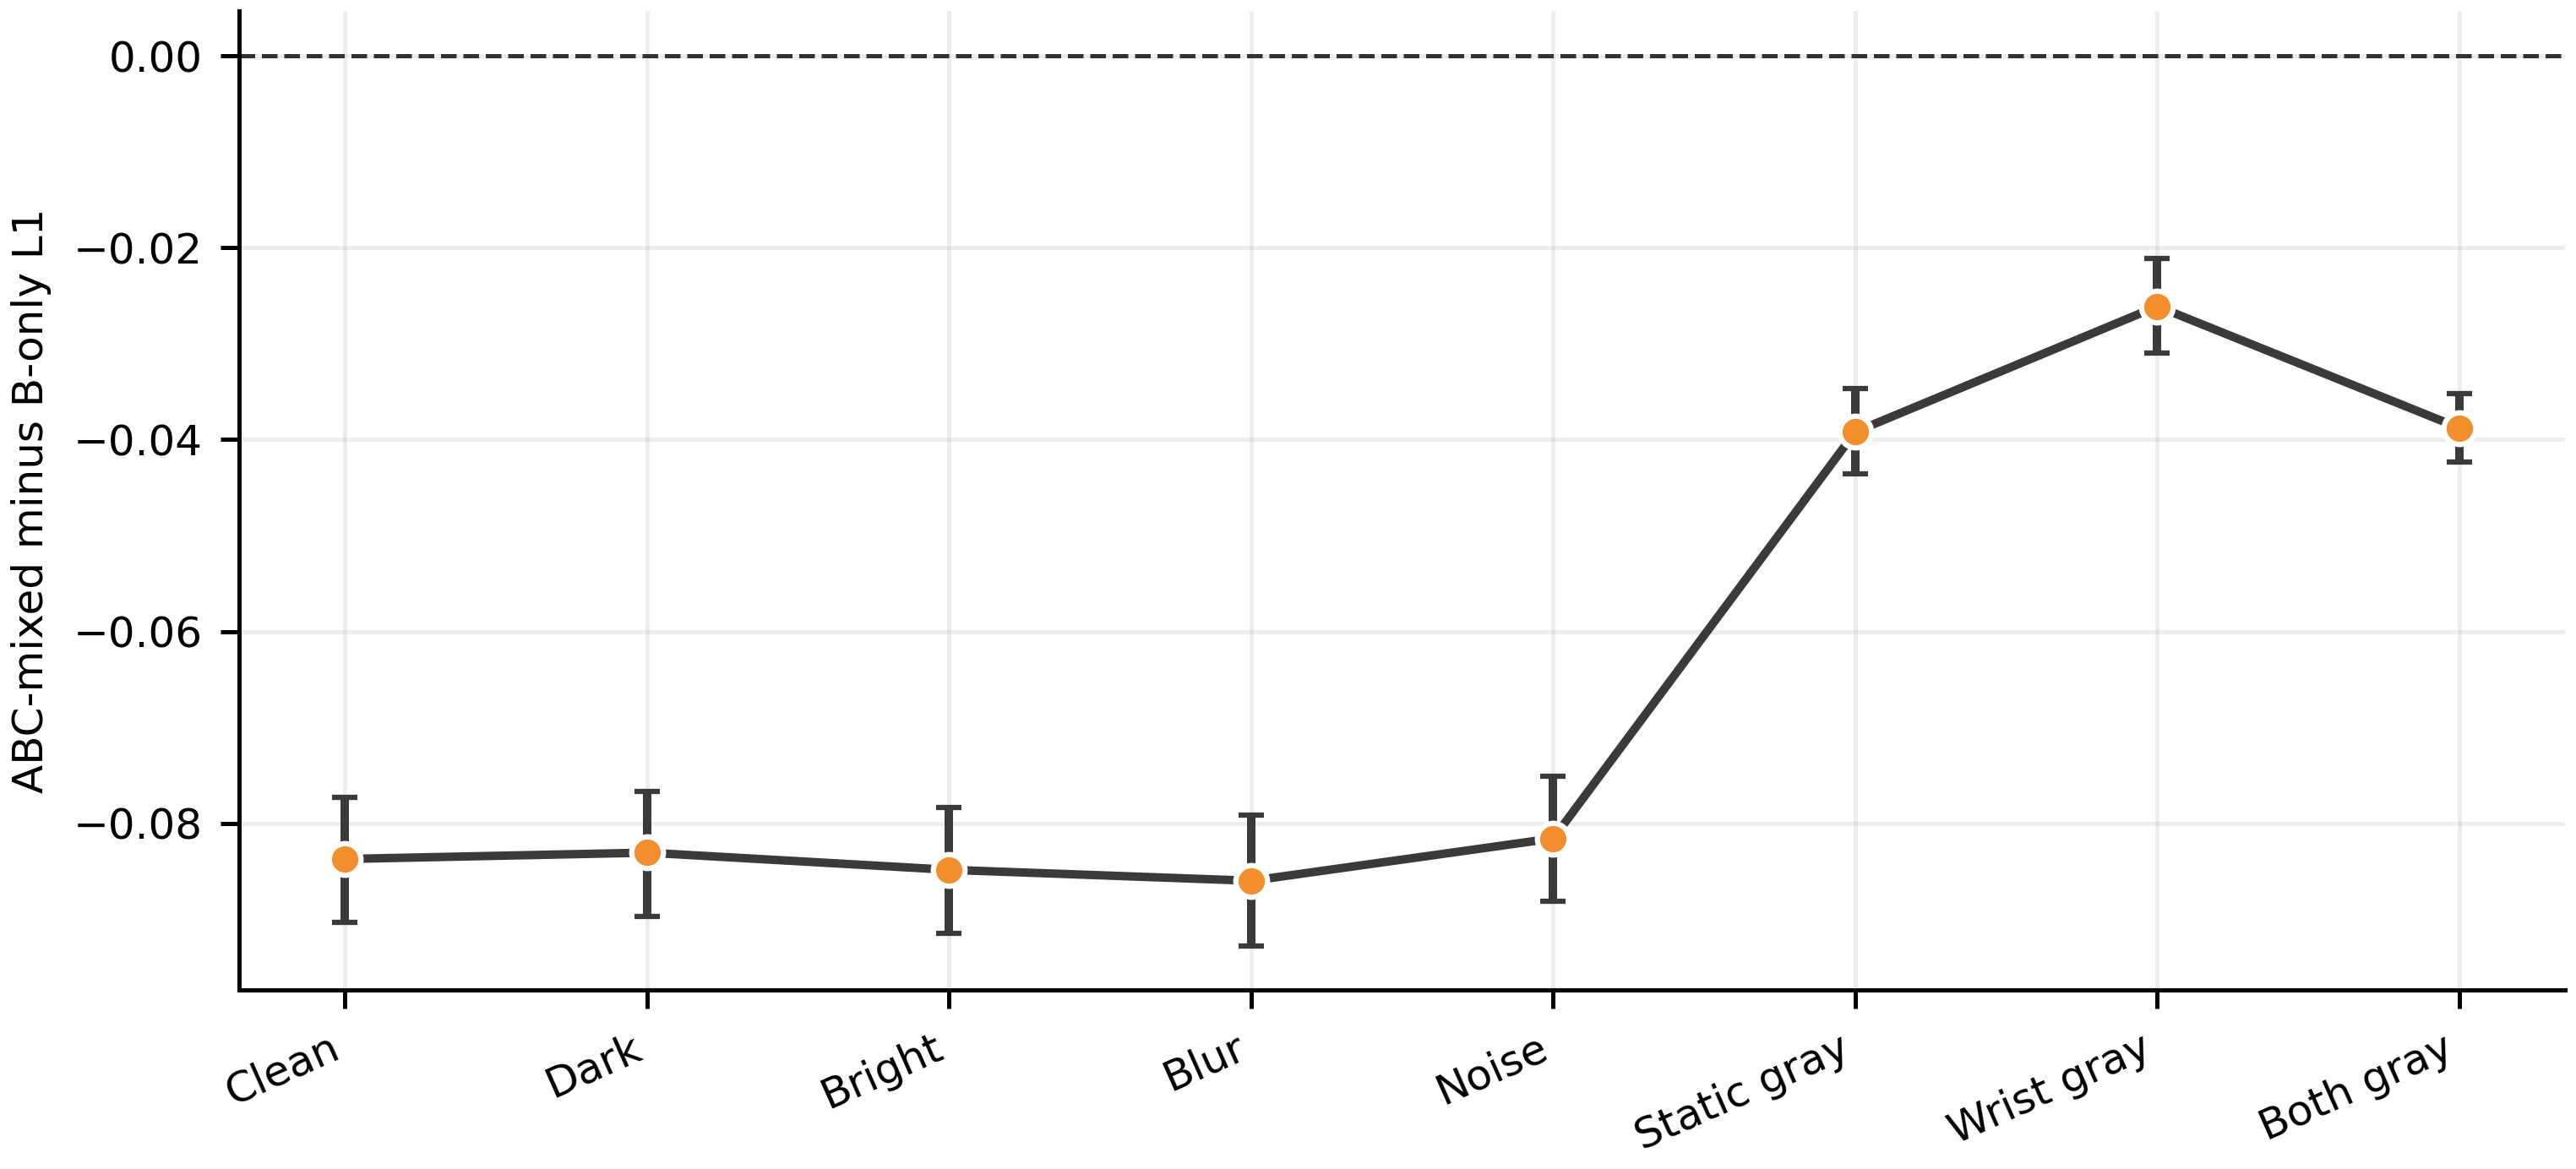
\includegraphics[width=\linewidth]{../figures/track2_extra/extra1024_visual_full_robustness_abc_minus_b_ci.png}
\end{minipage}
\caption{D-1024 offline 扰动的配对 bootstrap 95\% CI。左图为相对 clean 的误差增量；右图为 ABC-mixed visual 与 B-only visual 的 episode-level 差值，负值表示 ABC-mixed 更低。}
\label{fig:visual_shift_ci}
\end{figure}

动作维度热图进一步定位退化来源。图~\ref{fig:action_dim_shift} 中，wrist gray 对 ABC-mixed visual 的 gripper 和末端平移维度影响最明显；brightness、blur 的颜色接近零。遮掉 wrist camera 后，两组模型都失去接触区域信息，ABC-mixed 退化更大。

\begin{figure}[!htbp]
\centering
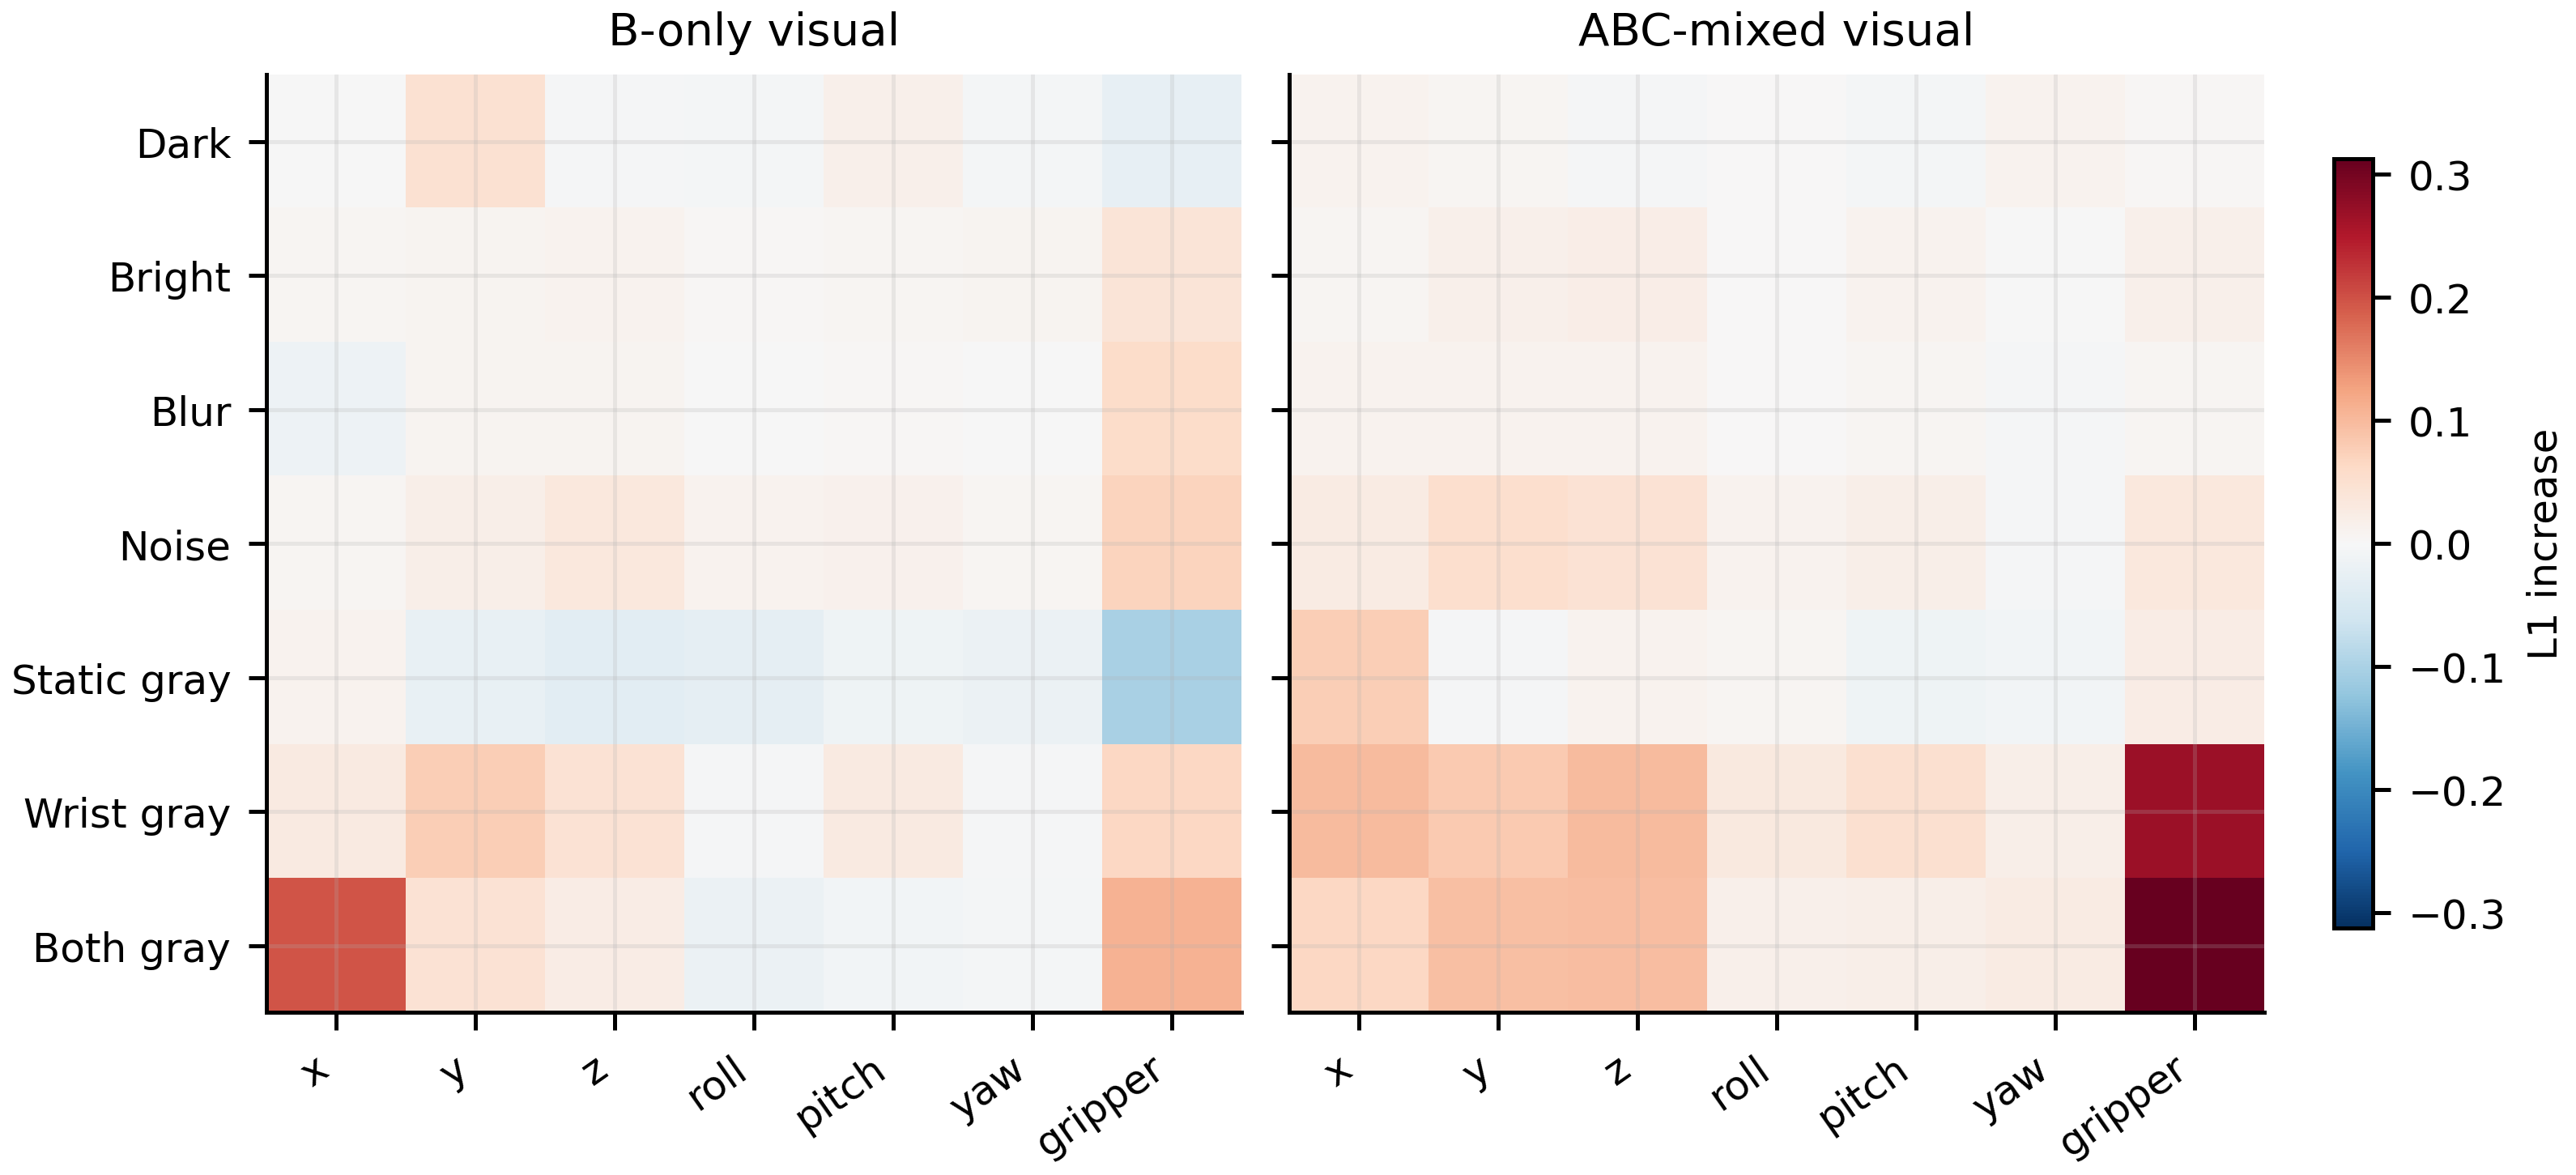
\includegraphics[width=0.92\linewidth]{../figures/track2_extra/extra1024_visual_full_robustness_action_dim_heatmap.png}
\caption{视觉扰动在动作维度上的影响。每个格子为对应扰动相对 clean 条件的 normalized \actionlone{} 增量。}
\label{fig:action_dim_shift}
\end{figure}

ACT 的输出动作块长度为 100，D-1024 子集中的有效专家标签覆盖位置 1--65，后续位置由 padding mask 移除。图~\ref{fig:chunk_prefix_l1} 统计 clean 条件下前 $n$ 个有效动作位置的 prefix \actionlone{}。ABC-mixed visual 在 $n=10/20/50/100$ 上分别为 0.522、0.538、0.570、0.574；B-only visual 对应为 0.607、0.628、0.653、0.654。随着 prefix 变长，两个模型都出现误差上升，ABC-mixed 的 tail/head ratio 为 1.26，B-only 为 1.11。ABC-mixed 的早段动作更准，后段 drift 更明显；这为后面的重规划频率实验提供了离线证据。

\begin{figure}[!htbp]
\centering
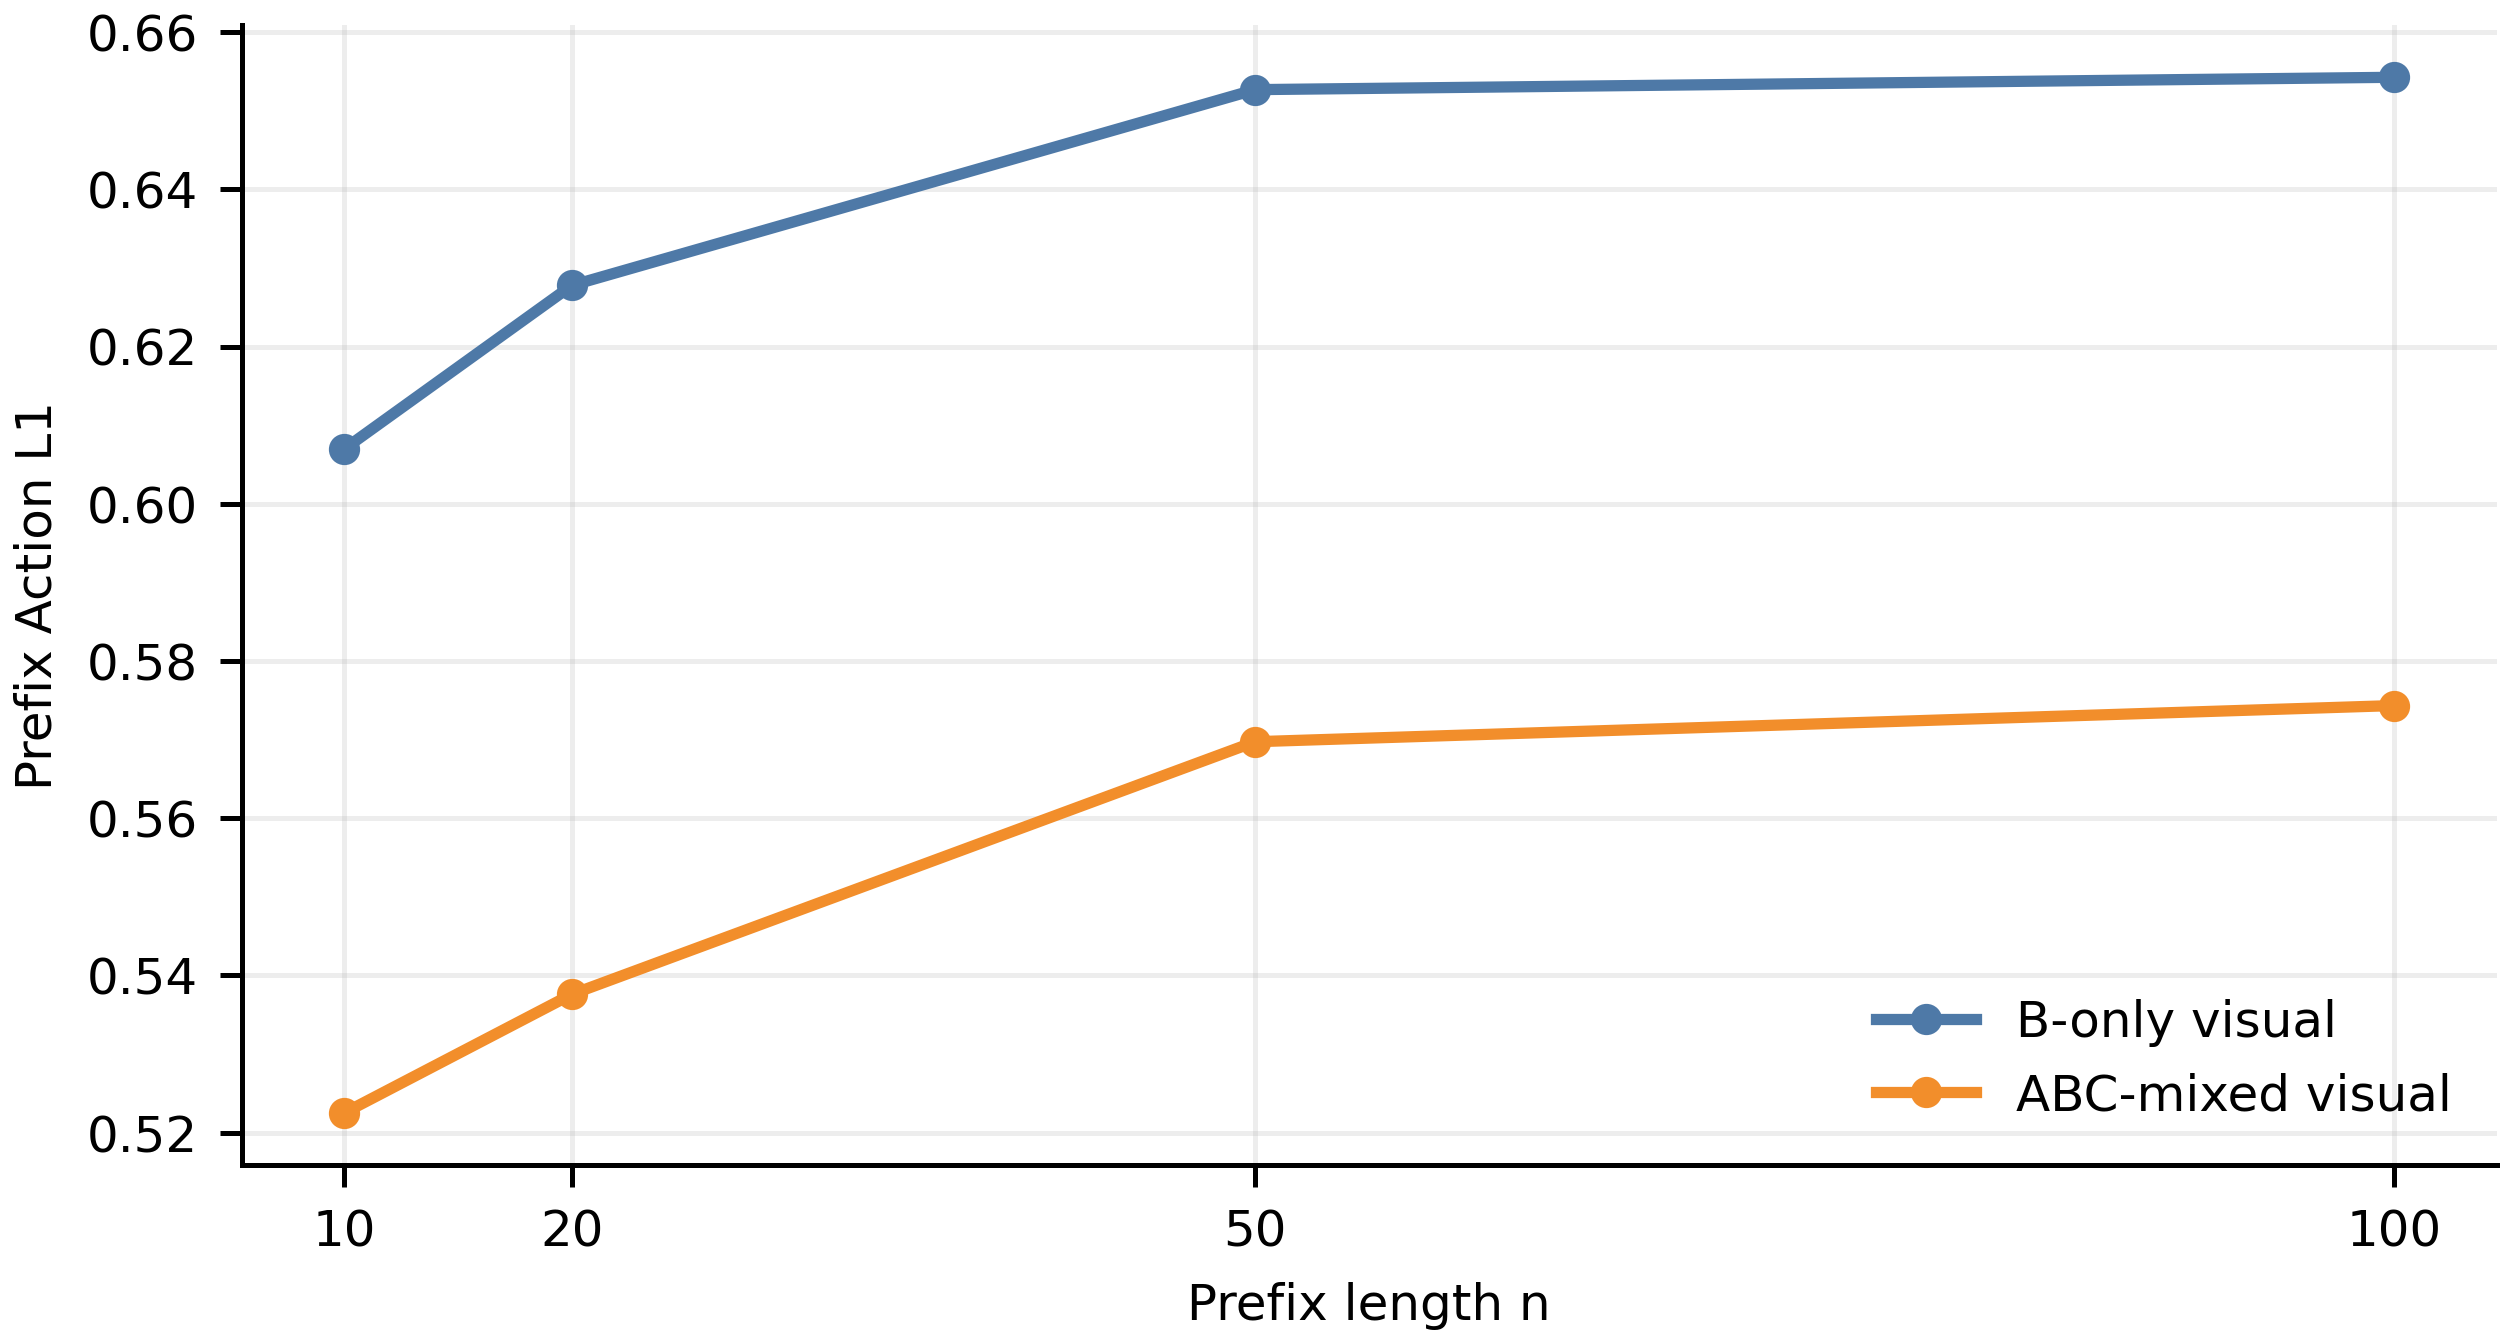
\includegraphics[width=0.72\linewidth]{../figures/track2_extra/extra1024_visual_full_robustness_chunk_prefix_l1.png}
\caption{clean 条件下 ACT 动作块 prefix \actionlone{}。$n=100$ 行实际使用有效位置 1--65；padding 后的位置不计入误差。}
\label{fig:chunk_prefix_l1}
\end{figure}

\begin{figure}[!htbp]
\centering
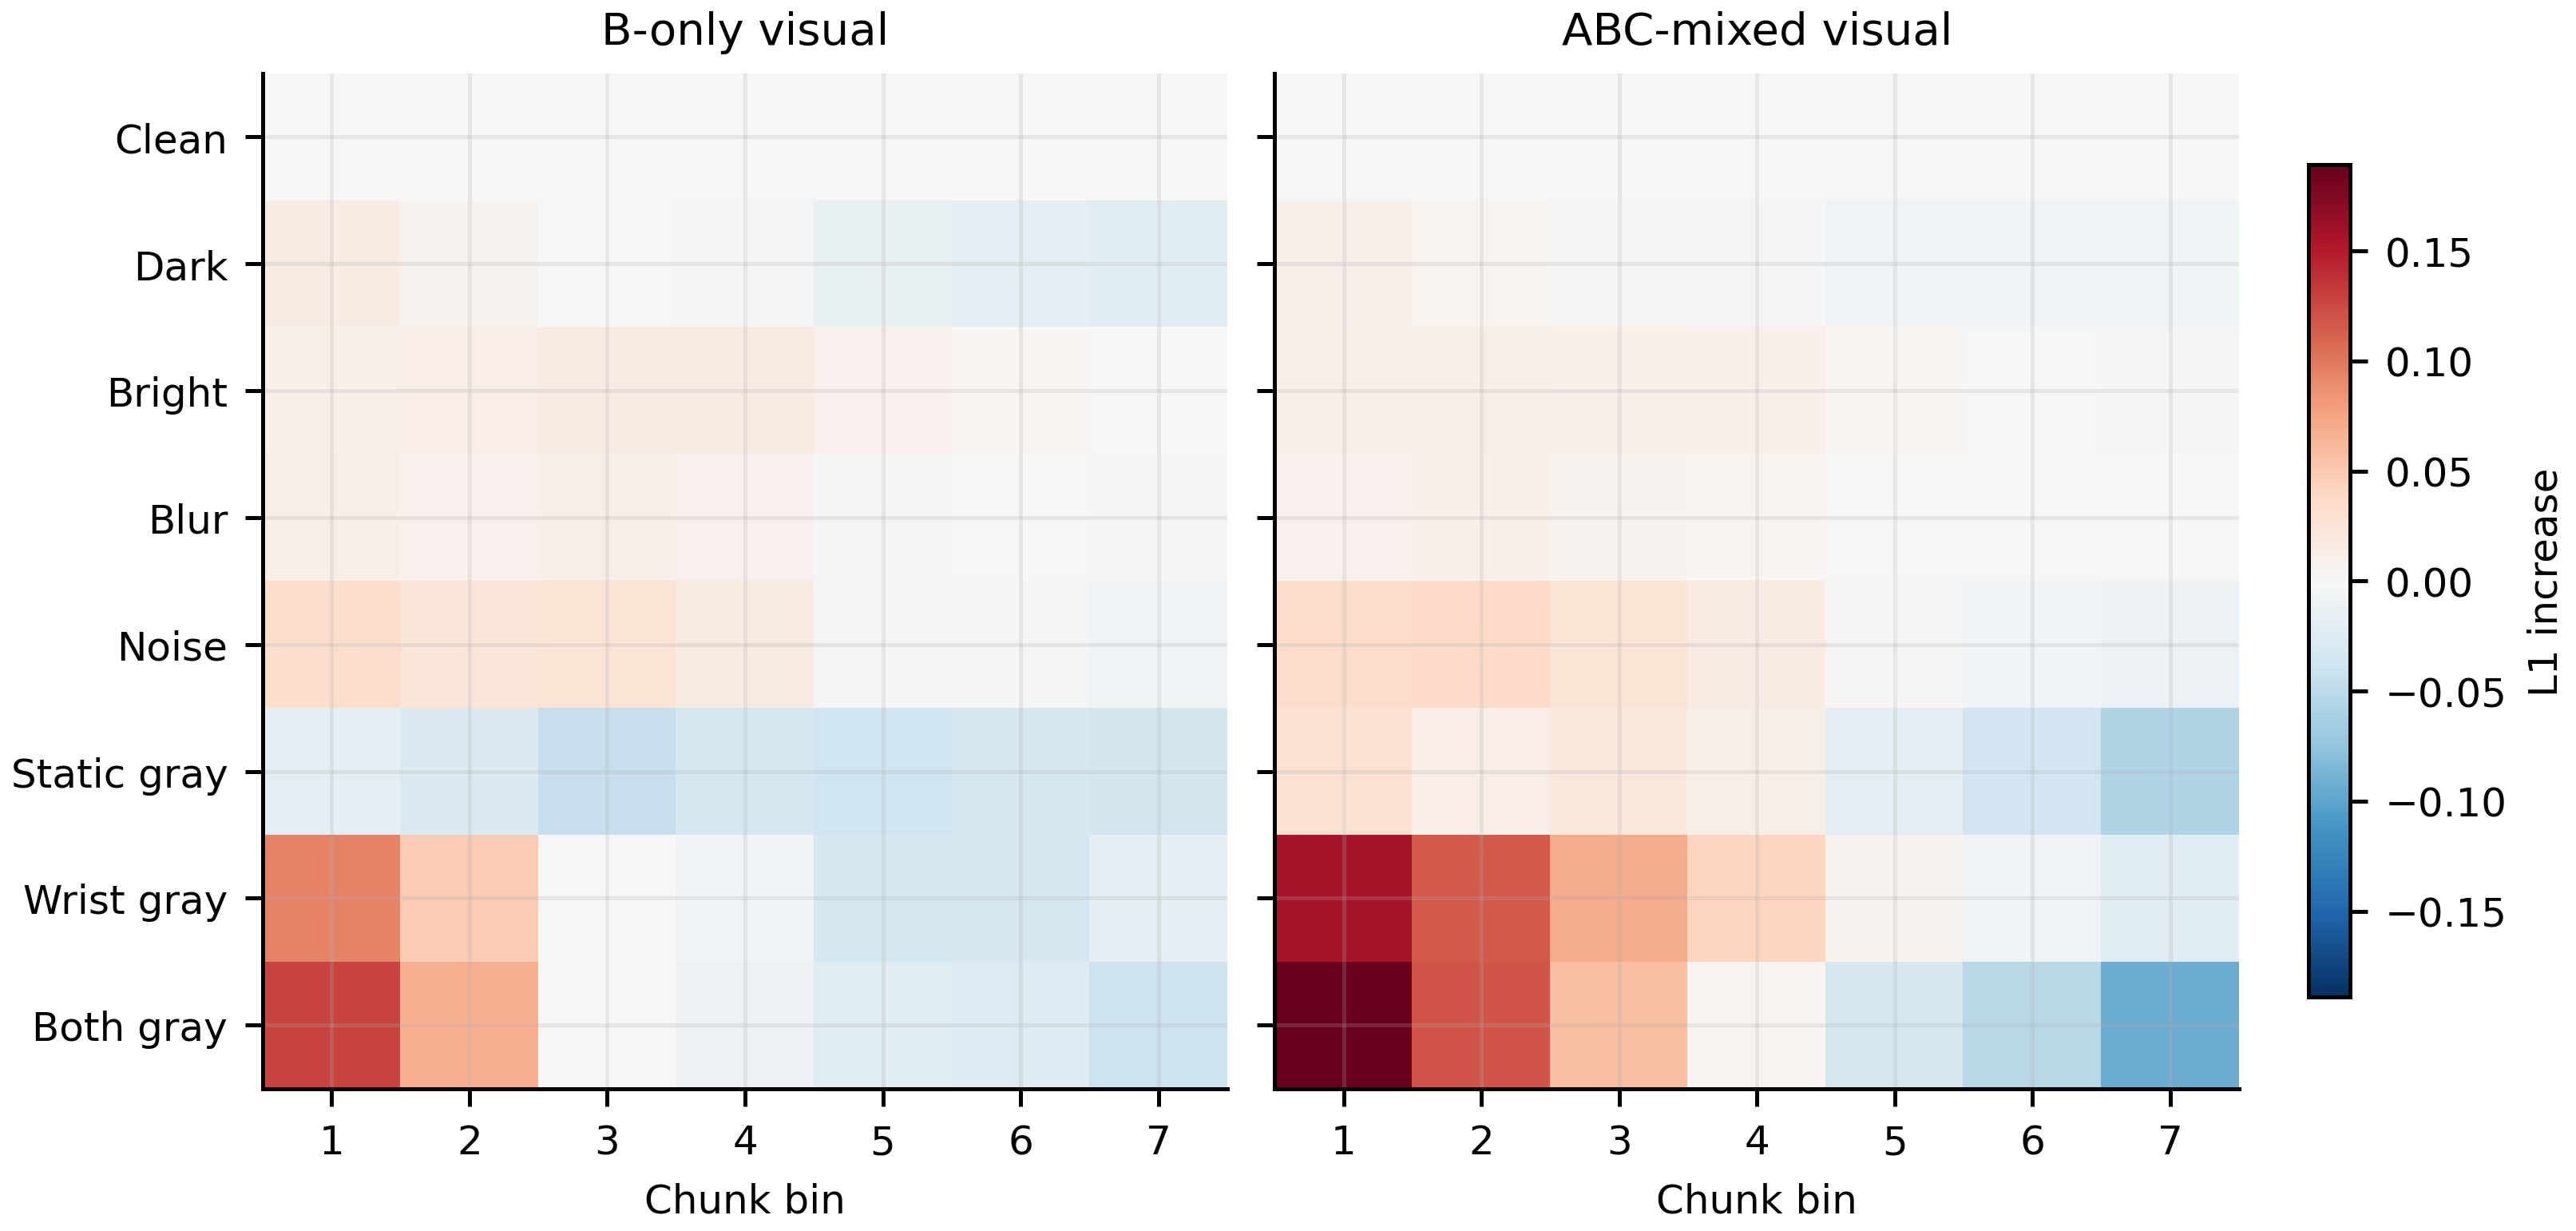
\includegraphics[width=0.92\linewidth]{../figures/track2_extra/extra1024_visual_full_robustness_chunk_condition_heatmap.png}
\caption{视觉扰动在 ACT chunk bin 上造成的 \actionlone{} 增量。wrist gray 和 both gray 在多个 bin 上产生更高误差，亮度和模糊扰动接近 clean。}
\label{fig:chunk_condition_heatmap}
\end{figure}

\FloatBarrier

\subsection{D 环境闭环执行}

闭环 rollout 记录策略在自己造成的状态分布中能完成多少子任务。表~\ref{tab:closed_loop_v2} 汇总 50 条 D 环境任务序列，每个子任务最多 360 步。两个 visual ACT 的平均完成子任务数均为 0.02；加入 task-id 后，B-only 达到 0.28，ABC-mixed 达到 0.68。离线 \actionlone{} 已经能分出 ABC-mixed 和 B-only 的强弱，闭环结果把任务目标缺失的代价放大：visual ACT 即使在专家轨迹附近动作误差不高，也很难在多任务链中持续选对动作。

\begin{table}[!htbp]
\centering
\small
\caption{D 环境 50 条序列闭环执行结果。Avg 为平均完成子任务数，SR@k 为至少连续完成 $k$ 个子任务的序列比例。}
\label{tab:closed_loop_v2}
\begin{tabular}{lcccccc}
\toprule
模型 & Avg $\uparrow$ & SR@1 $\uparrow$ & SR@2 $\uparrow$ & SR@3 $\uparrow$ & SR@4 $\uparrow$ & SR@5 $\uparrow$ \\
\midrule
B-only visual ACT & 0.02 & 0.02 & 0.00 & 0.00 & 0.00 & 0.00 \\
ABC-mixed visual ACT & 0.02 & 0.02 & 0.00 & 0.00 & 0.00 & 0.00 \\
B-only task-id ACT & 0.28 & 0.20 & 0.06 & 0.02 & 0.00 & 0.00 \\
ABC-mixed task-id ACT & \best{0.68} & \best{0.42} & \best{0.18} & \best{0.08} & 0.00 & 0.00 \\
\bottomrule
\end{tabular}
\end{table}

平均值之外，闭环日志还能看到每条序列的具体变化。图~\ref{fig:closed_loop_outcome_heatmap} 把同一批 50 条 D 环境序列按列展开：两个 visual ACT 几乎整行停在 0/5；加入 task-id 后开始出现 1--3 个完成子任务；ABC-mixed task-id 在 $n=20$ 下出现 4 条 5/5 序列。成功提升覆盖多条任务链，而不是由个别异常序列拉高平均值。

\begin{figure}[!htbp]
\centering
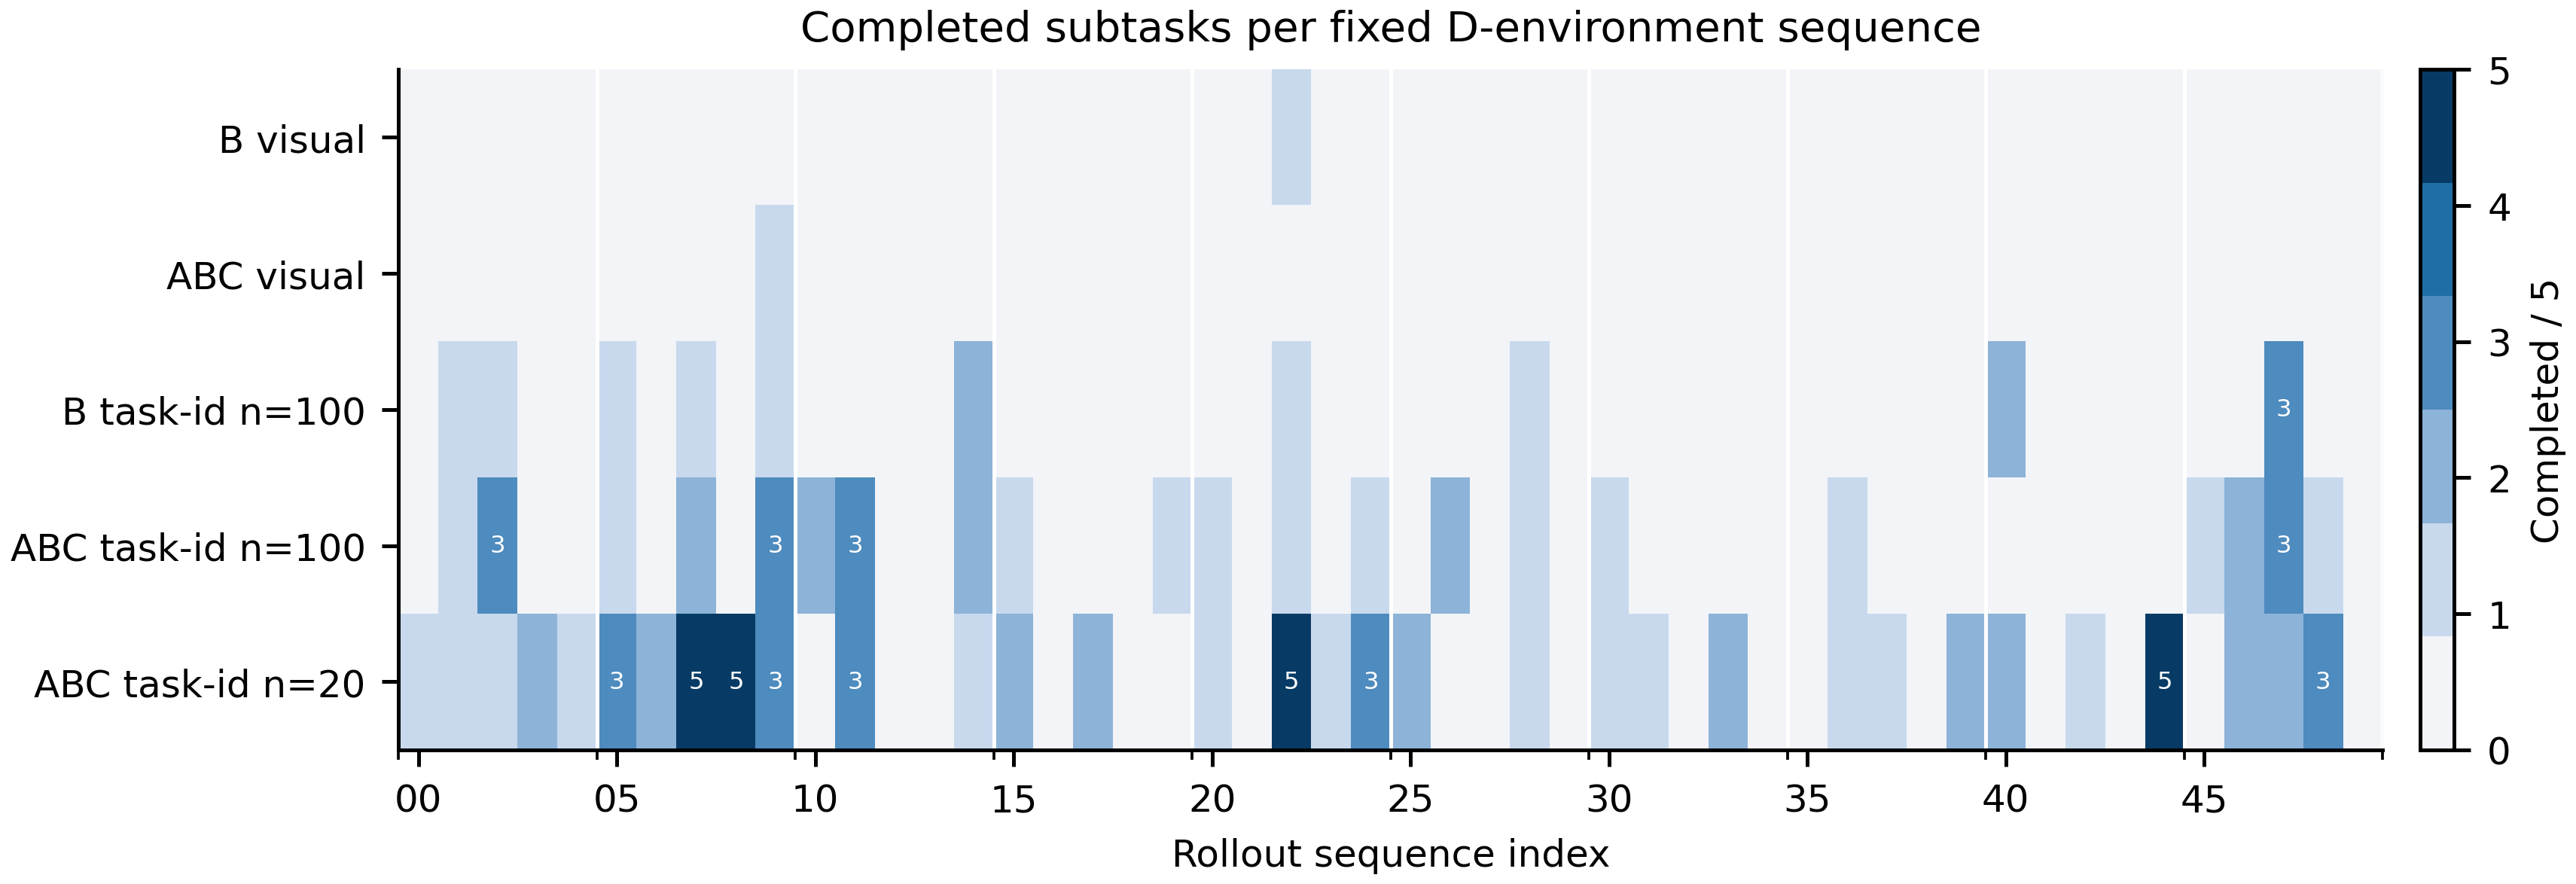
\includegraphics[width=\linewidth]{../figures/track2_extra/extra1024_closed_loop_outcome_heatmap.png}
\caption{同一批 50 条 D 环境序列上的完成子任务数。每列是一条固定初始状态和任务链的 rollout，颜色表示该模型完成 0--5 个子任务。}
\label{fig:closed_loop_outcome_heatmap}
\end{figure}

\begin{figure}[!htbp]
\centering
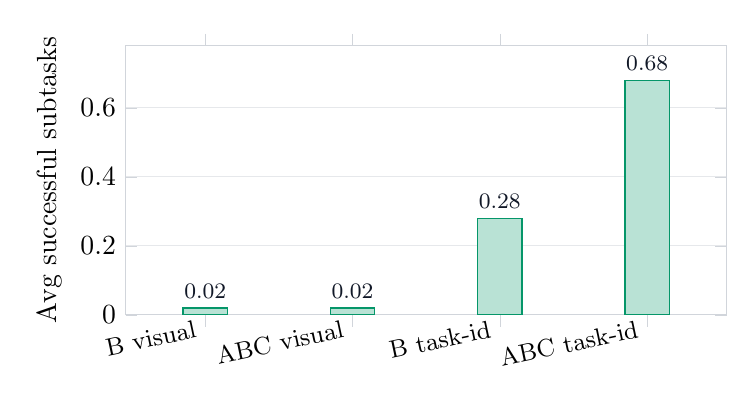
\begin{tikzpicture}
\begin{axis}[
  width=0.76\linewidth,
  height=5.0cm,
  ybar,
  bar width=16pt,
  ymin=0,
  ymax=0.78,
  symbolic x coords={B visual,ABC visual,B task-id,ABC task-id},
  xtick=data,
  ylabel={Avg successful subtasks},
  xticklabel style={font=\small, rotate=12, anchor=east},
  ymajorgrids=true,
  grid style={draw=linegray!55},
  axis line style={draw=linegray},
  tick style={draw=linegray},
  point meta=y,
  nodes near coords={\pgfmathprintnumber[fixed,precision=2]{\pgfplotspointmeta}},
  every node near coord/.append style={font=\footnotesize, text=ink},
  enlarge x limits=0.18,
]
\addplot+[draw=taskgreen, fill=taskgreen!28] coordinates {
  (B visual,0.02)
  (ABC visual,0.02)
  (B task-id,0.28)
  (ABC task-id,0.68)
};
\end{axis}
\end{tikzpicture}
\caption{D 环境闭环平均完成子任务数。visual ACT 接近全零；task-id ACT 出现可观测成功。}
\label{fig:closed_loop_avg_v2}
\end{figure}

图~\ref{fig:metric_bridge} 把四个主模型放到同一个 offline/closed-loop 坐标系中。ABC-mixed visual 的 D \actionlone{} 已明显低于 B-only visual，但两个 visual 模型的闭环平均完成数仍停在 0.02；task-id 模型沿纵轴打开差距，ABC-mixed task-id 同时位于更低 \actionlone{} 和更高闭环完成数的位置。该图把离线动作拟合和多任务执行拆开看：视觉覆盖降低动作误差，任务条件决定策略能否在长链执行中持续选对操作。

\begin{figure}[!htbp]
\centering
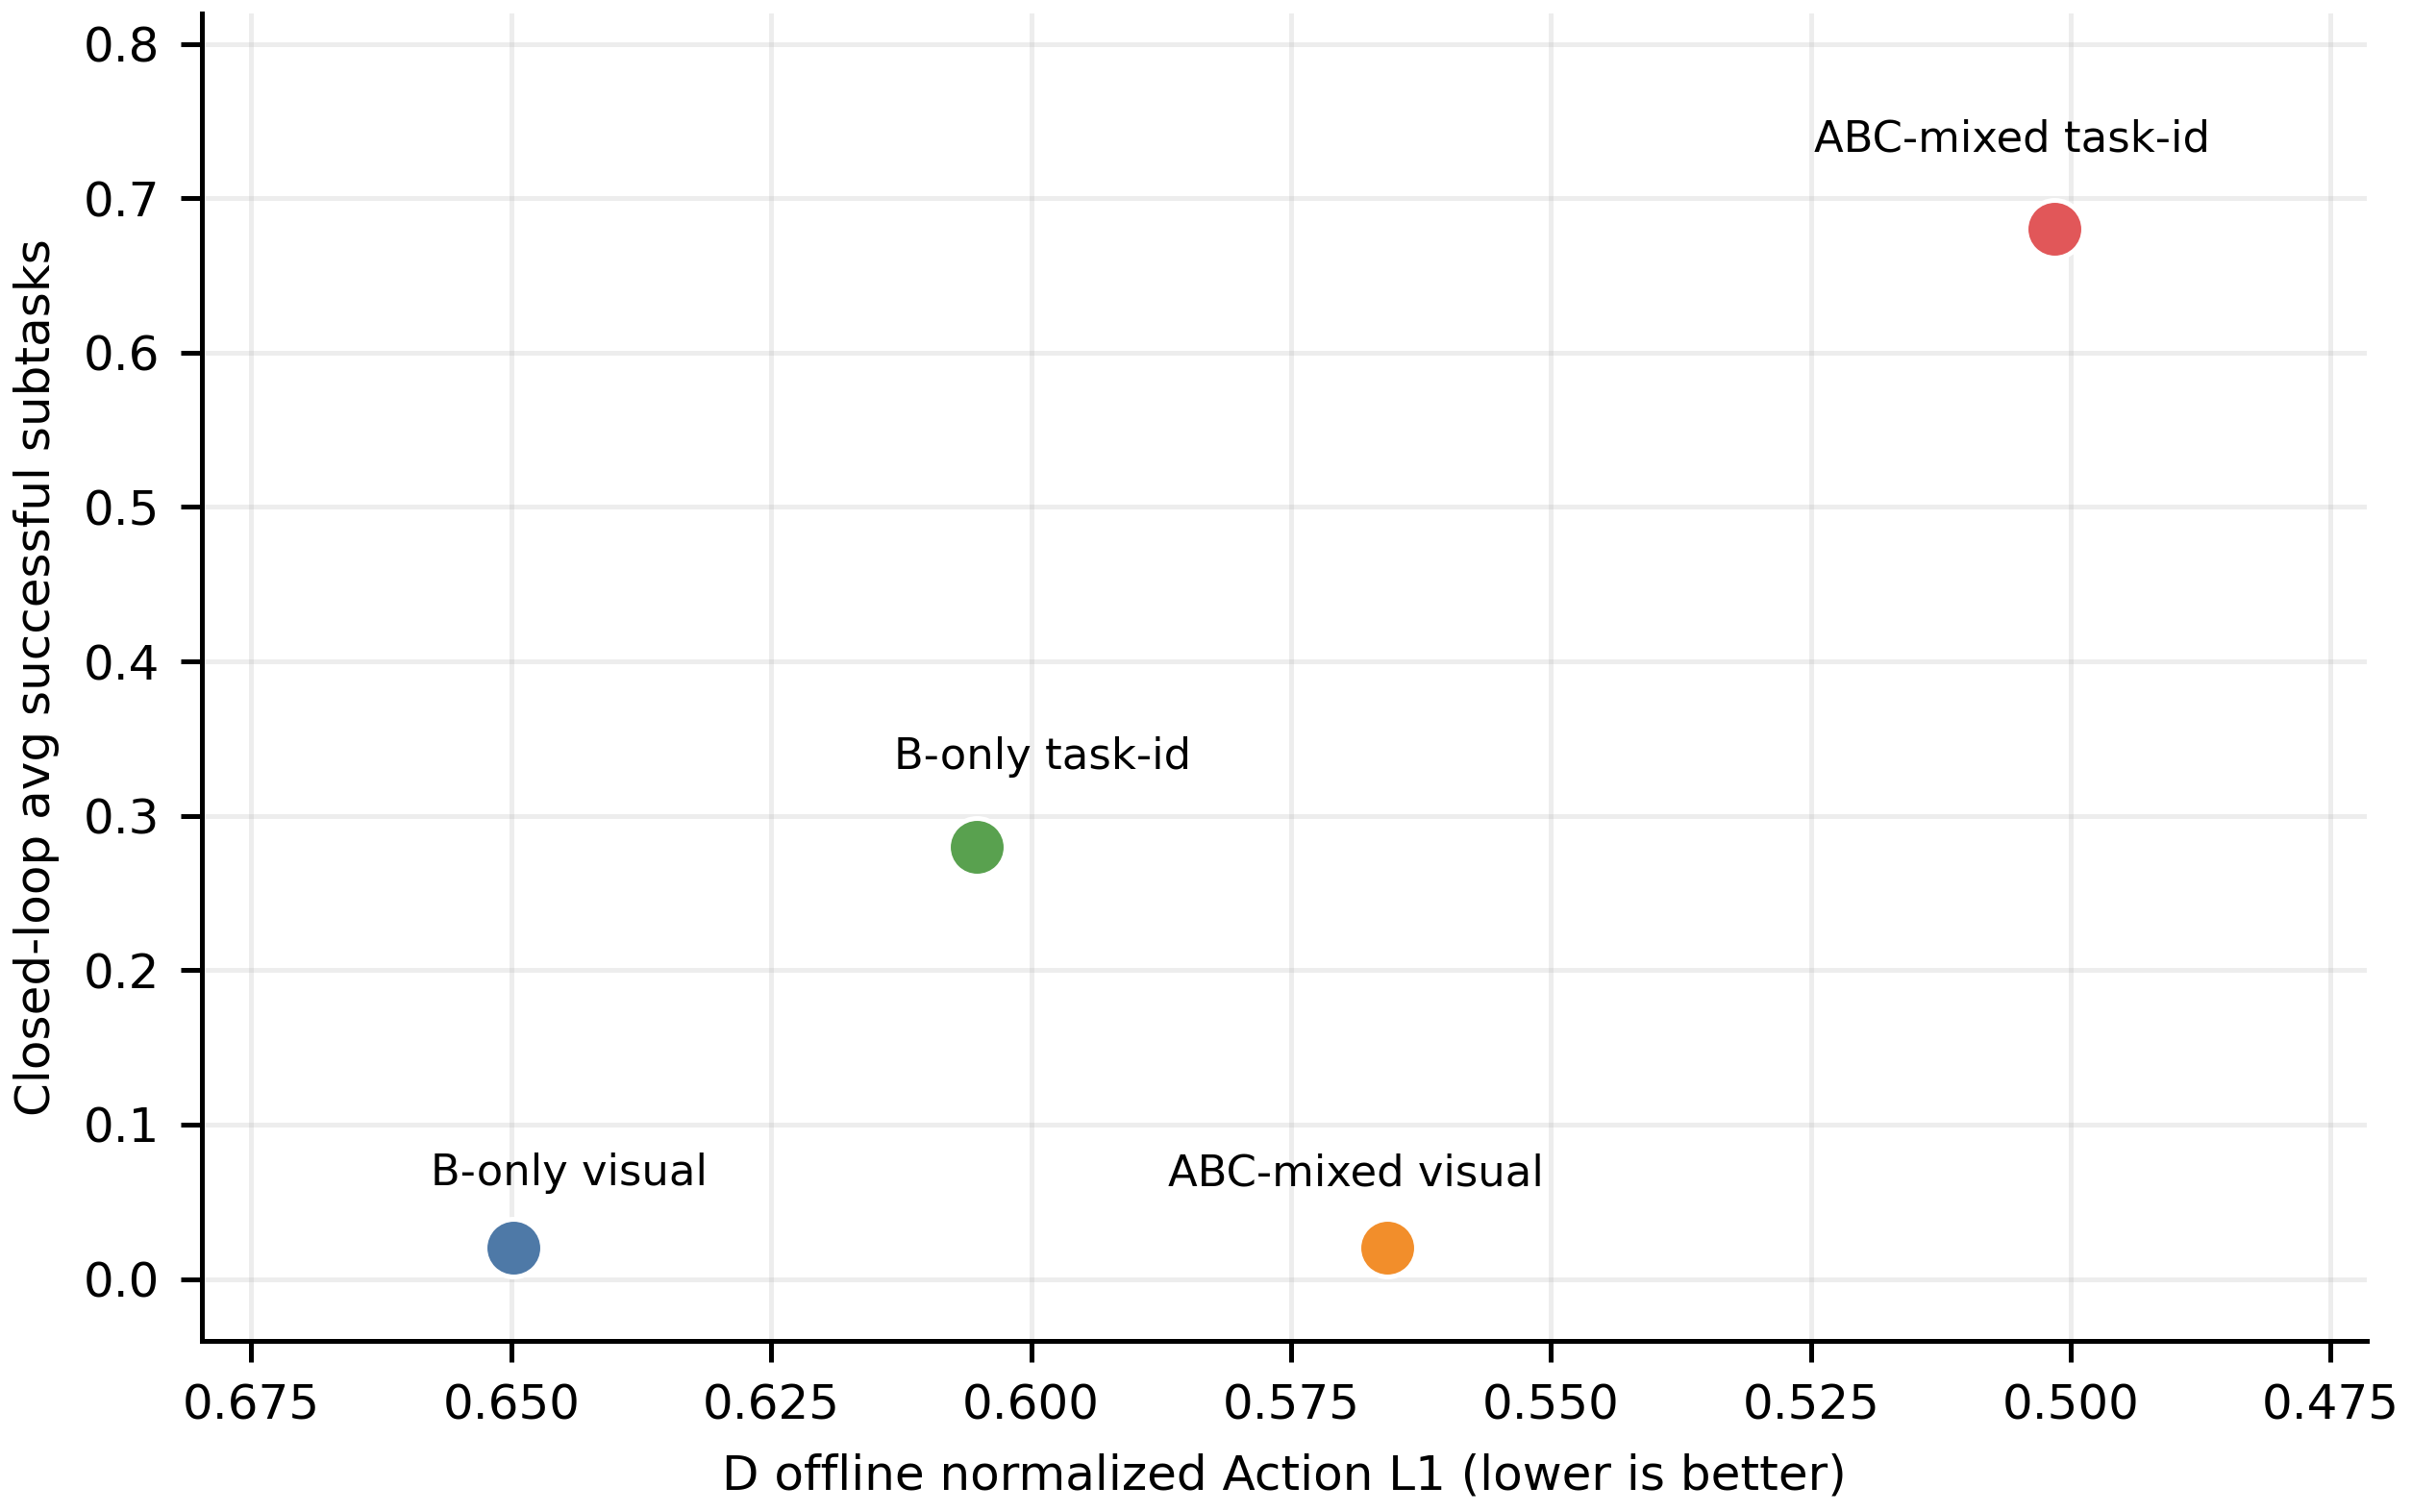
\includegraphics[width=0.72\linewidth]{../figures/track2_extra/extra1024_metric_bridge_offline_to_closed_loop.png}
\caption{D 环境离线 \actionlone{} 与闭环平均完成子任务数。横轴反向显示，越靠右表示离线动作误差越低。}
\label{fig:metric_bridge}
\end{figure}

50 条序列的闭环样本有限，我们对 successful-subtasks 向量做 10000 次 bootstrap。ABC-mixed task-id 默认 $n=100$ 的平均完成数为 0.68，95\% CI 为 [0.44, 0.96]；B-only task-id 对应为 0.28，CI 集中在低值区间。图~\ref{fig:closed_loop_qual} 展示同一条 seq\_11 在四个模型上的关键帧：B visual、ABC visual 和 B-only task-id 都停在 0/5，ABC-mixed task-id 完成 3/5。定量表和关键帧给出的判断一致，任务条件输入改变了策略在同一观测下的动作选择。

\begin{figure}[!htbp]
\centering
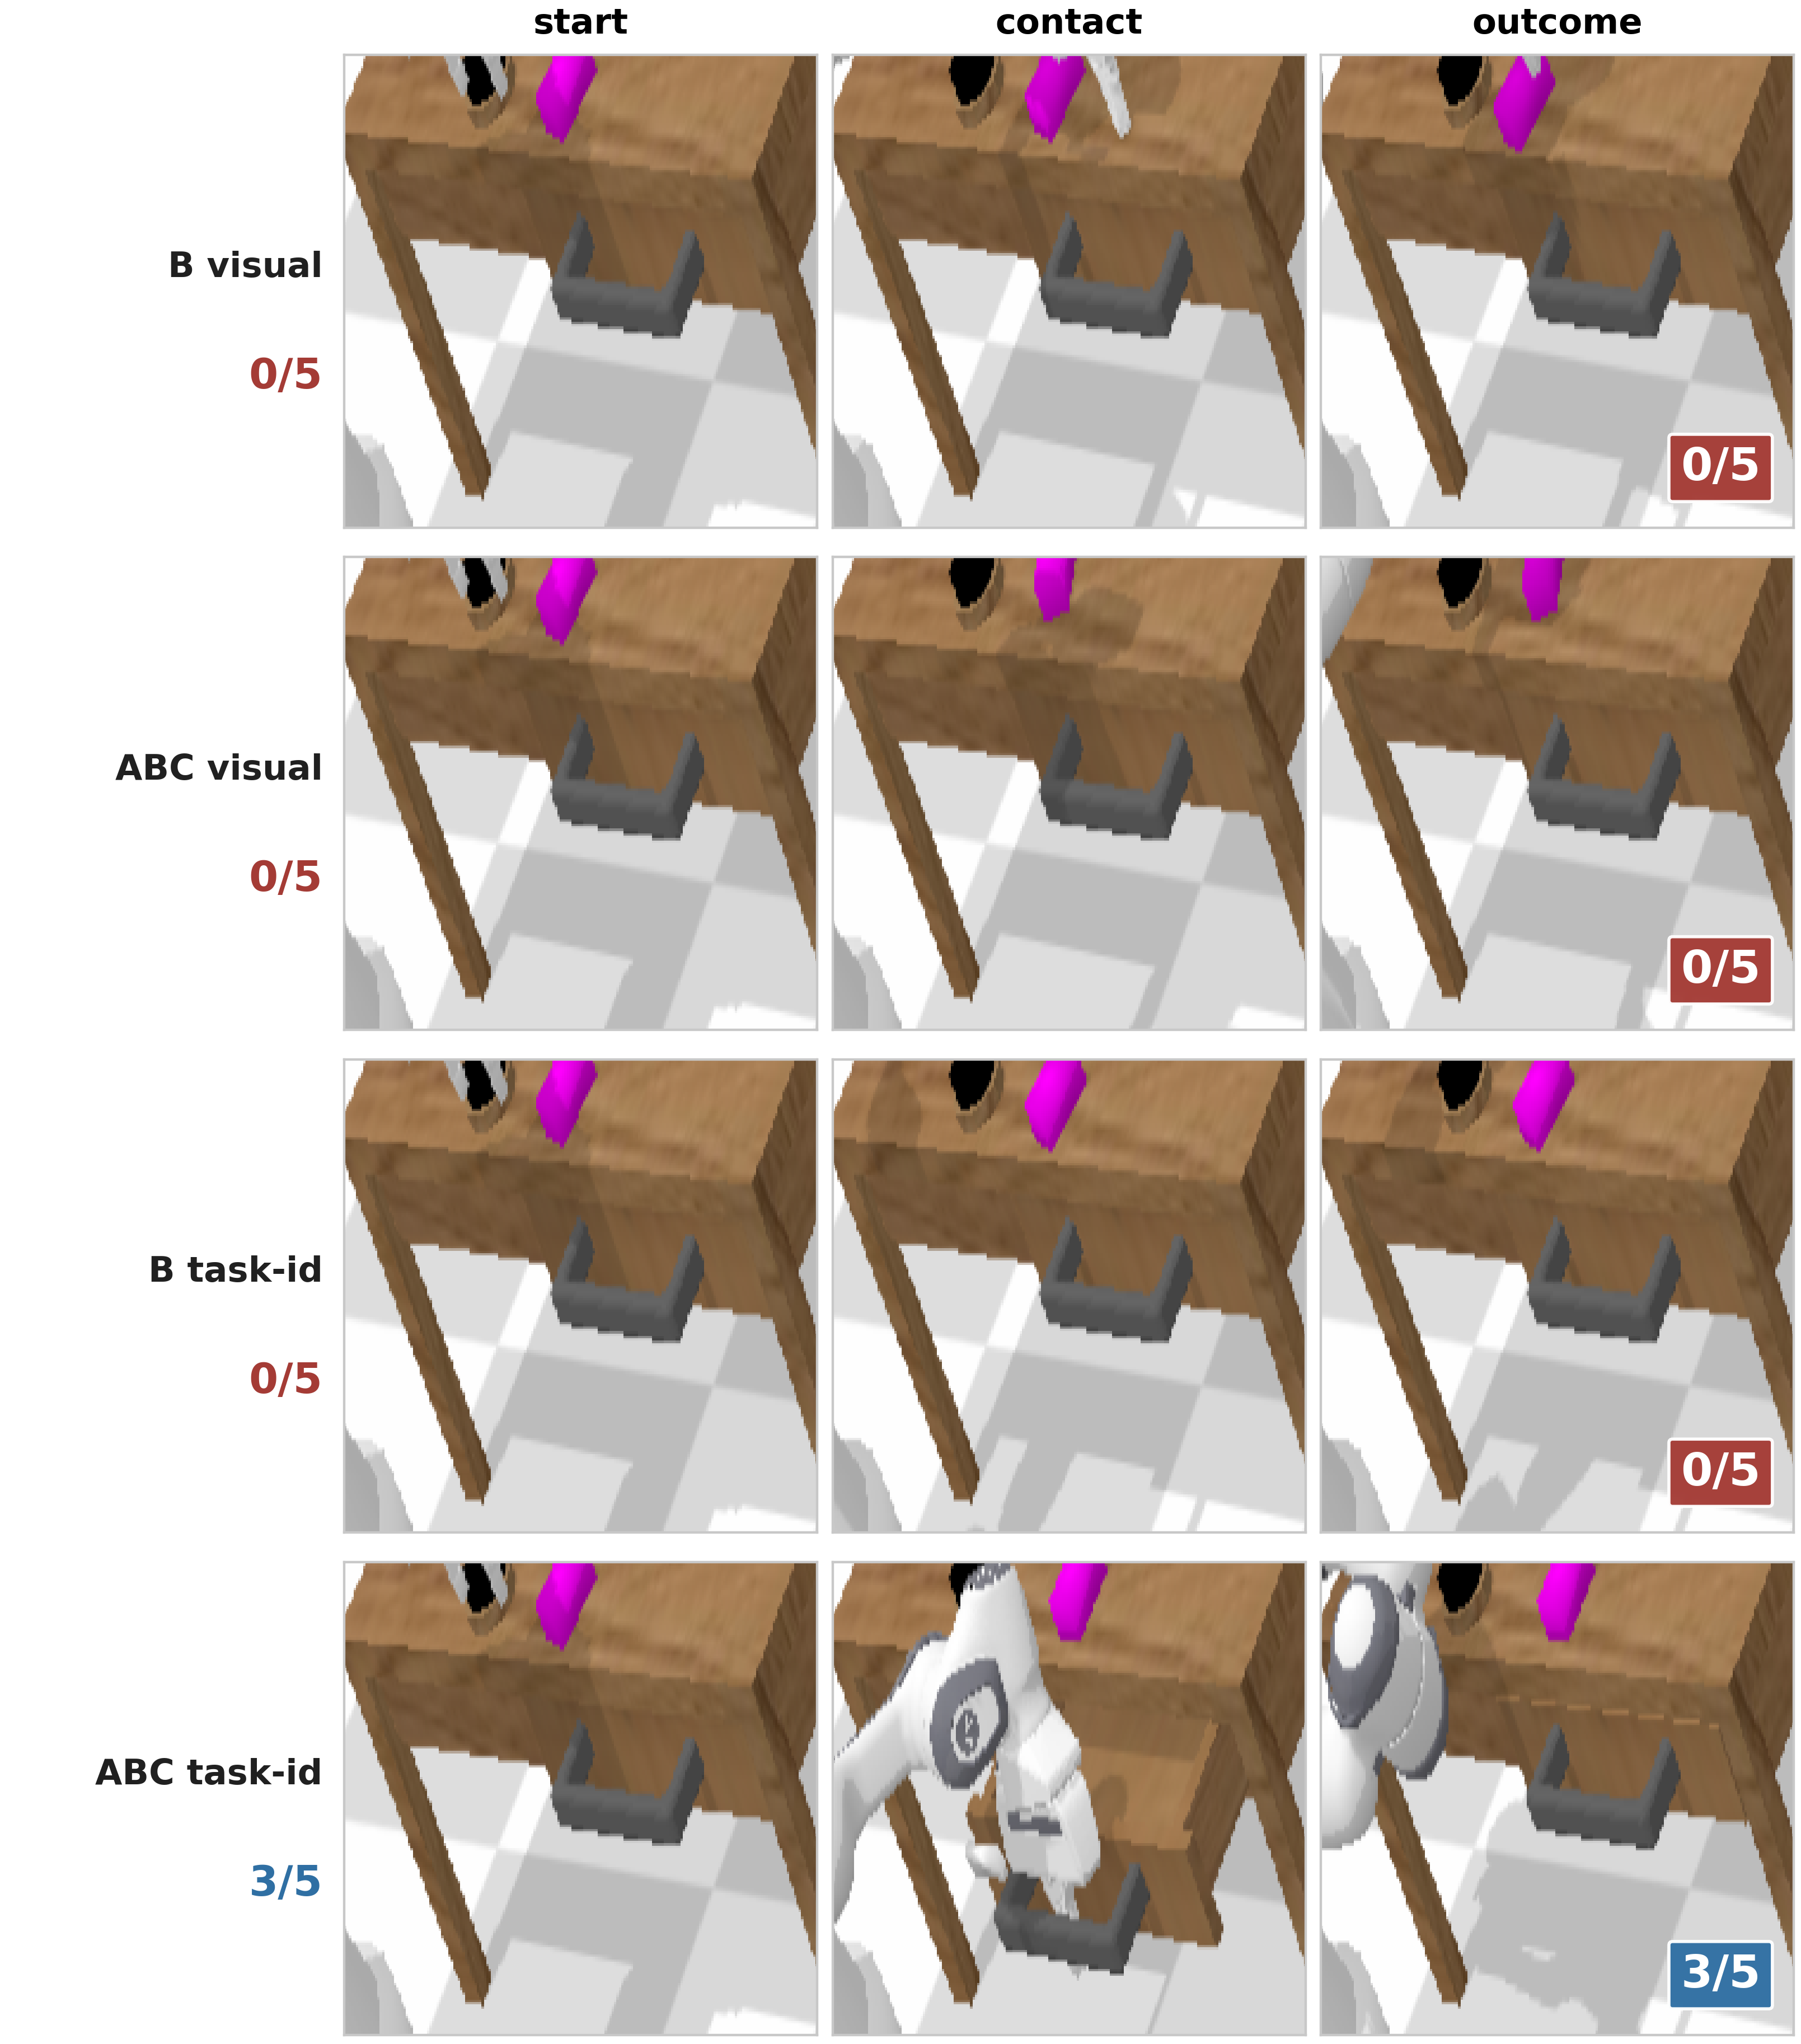
\includegraphics[width=0.68\linewidth]{../figures/track2_extra/rollout_seq_11_four_model_keyframes.png}
\caption{seq\_11 的四模型闭环关键帧。三列分别为 start、contact 和 outcome；outcome 图中直接标注该 rollout 完成的子任务数。}
\label{fig:closed_loop_qual}
\end{figure}

成功步数分布说明，120-step horizon 并不会截断所有成功，但会漏记一部分晚出现的真实成功。图~\ref{fig:success_step_dist} 只统计已经成功的子任务，ABC-mixed task-id 在 $n=20$ 下共有 68 个成功子任务，其中 12 个发生在 120 步之后；默认 $n=100$ 有 34 个成功子任务，其中 10 个超过 120 步。旧的 120-step 设置会把这部分真实成功记为失败，尤其会低估接触后推进、拉动和放置这类慢完成任务。

\begin{figure}[!htbp]
\centering
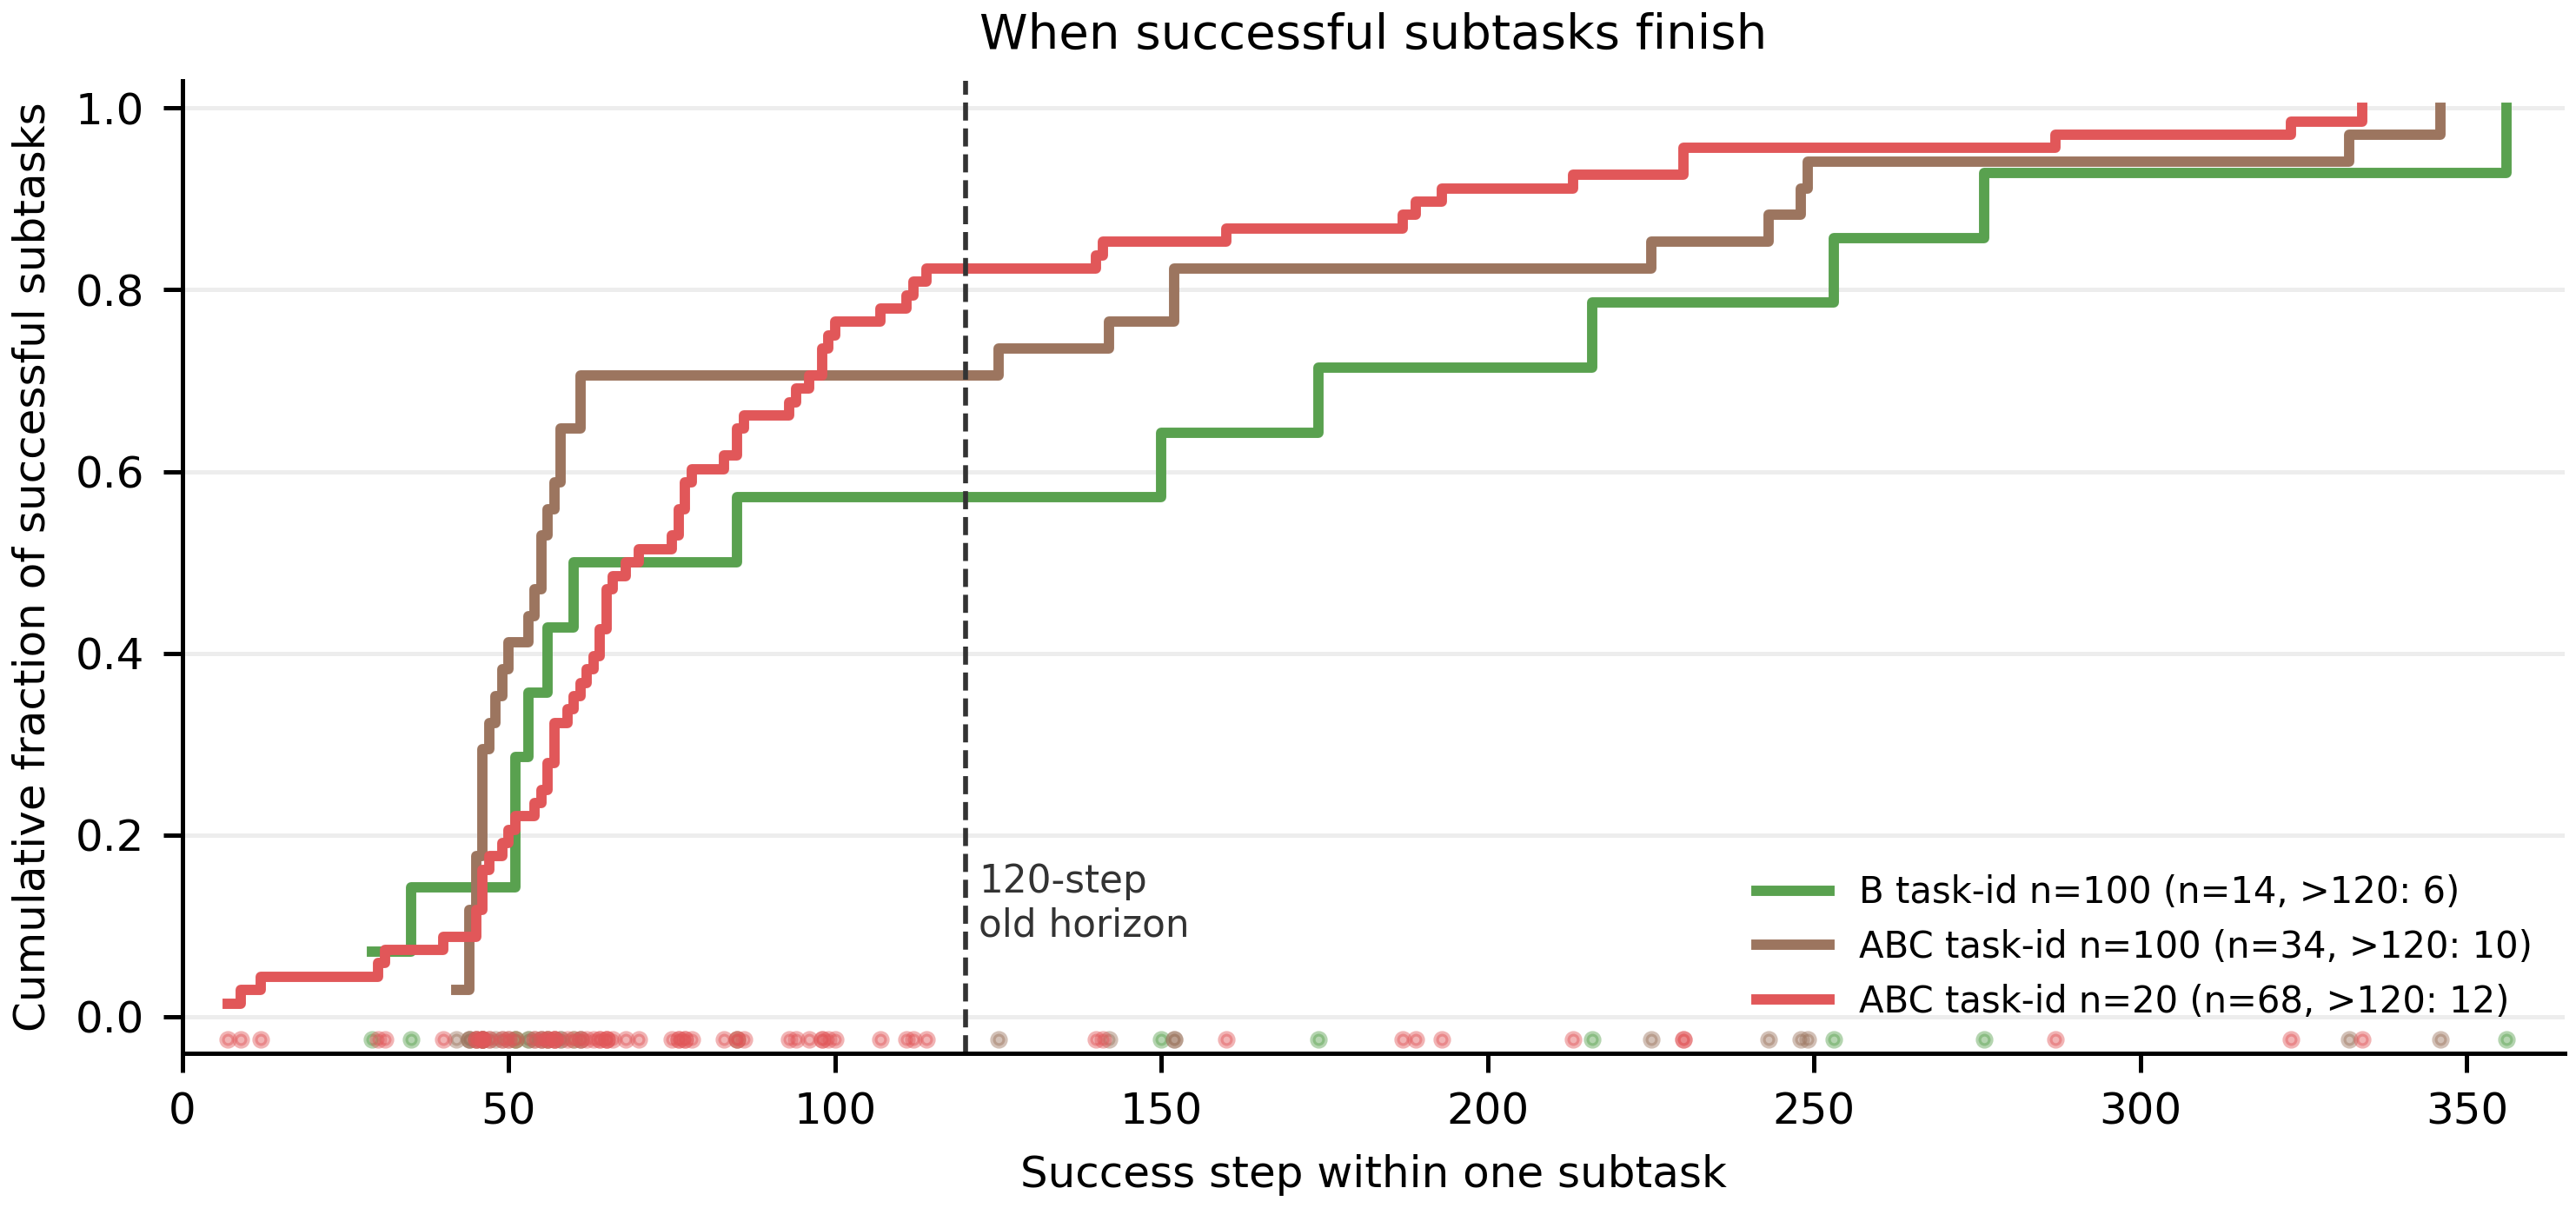
\includegraphics[width=0.82\linewidth]{../figures/track2_extra/extra1024_closed_loop_success_step_distribution.png}
\caption{成功子任务的完成步数分布。虚线为早期诊断使用过的 120-step horizon；曲线只统计 oracle 判定成功的子任务。}
\label{fig:success_step_dist}
\end{figure}

\FloatBarrier

\subsection{Action chunking 与视觉偏移鲁棒性}

ACT 训练阶段固定 chunk size 为 100，消融只改变推理时执行多少步后重新观测。表~\ref{tab:chunking_v2} 给出 $n_\text{action steps}=10,20,50,100$ 的 50-sequence rollout。ABC-mixed task-id 在默认 $n=100$ 时平均完成 0.68 个子任务，$n=20$ 时提升到 1.36；$n=10$ 回落到 0.98。B-only task-id 在 0.20--0.28 之间波动，没有形成稳定上升。重规划频率能利用新的图像反馈修正动作块 drift，但它依赖前面的视觉表征质量。

\begin{table}[!htbp]
\centering
\footnotesize
\caption{Action chunking 消融。训练 chunk size 固定为 100，推理时改变 $n_\text{action steps}$。}
\label{tab:chunking_v2}
\begin{tabular}{llccccc}
\toprule
模型 & $n_\text{action steps}$ & Avg $\uparrow$ & SR@1 & SR@2 & SR@3 & SR@5 \\
\midrule
B-only task-id ACT & 10 & 0.28 & 0.26 & 0.02 & 0.00 & 0.00 \\
B-only task-id ACT & 20 & 0.24 & 0.20 & 0.04 & 0.00 & 0.00 \\
B-only task-id ACT & 50 & 0.20 & 0.18 & 0.02 & 0.00 & 0.00 \\
B-only task-id ACT & 100 & 0.28 & 0.20 & 0.06 & 0.02 & 0.00 \\
\midrule
ABC-mixed task-id ACT & 10 & 0.98 & 0.50 & 0.30 & 0.10 & 0.04 \\
ABC-mixed task-id ACT & 20 & \best{1.36} & \best{0.64} & \best{0.38} & \best{0.18} & \best{0.08} \\
ABC-mixed task-id ACT & 50 & 0.88 & 0.56 & 0.24 & 0.06 & 0.00 \\
ABC-mixed task-id ACT & 100 & 0.68 & 0.42 & 0.18 & 0.08 & 0.00 \\
\bottomrule
\end{tabular}
\end{table}

\begin{figure}[!htbp]
\centering
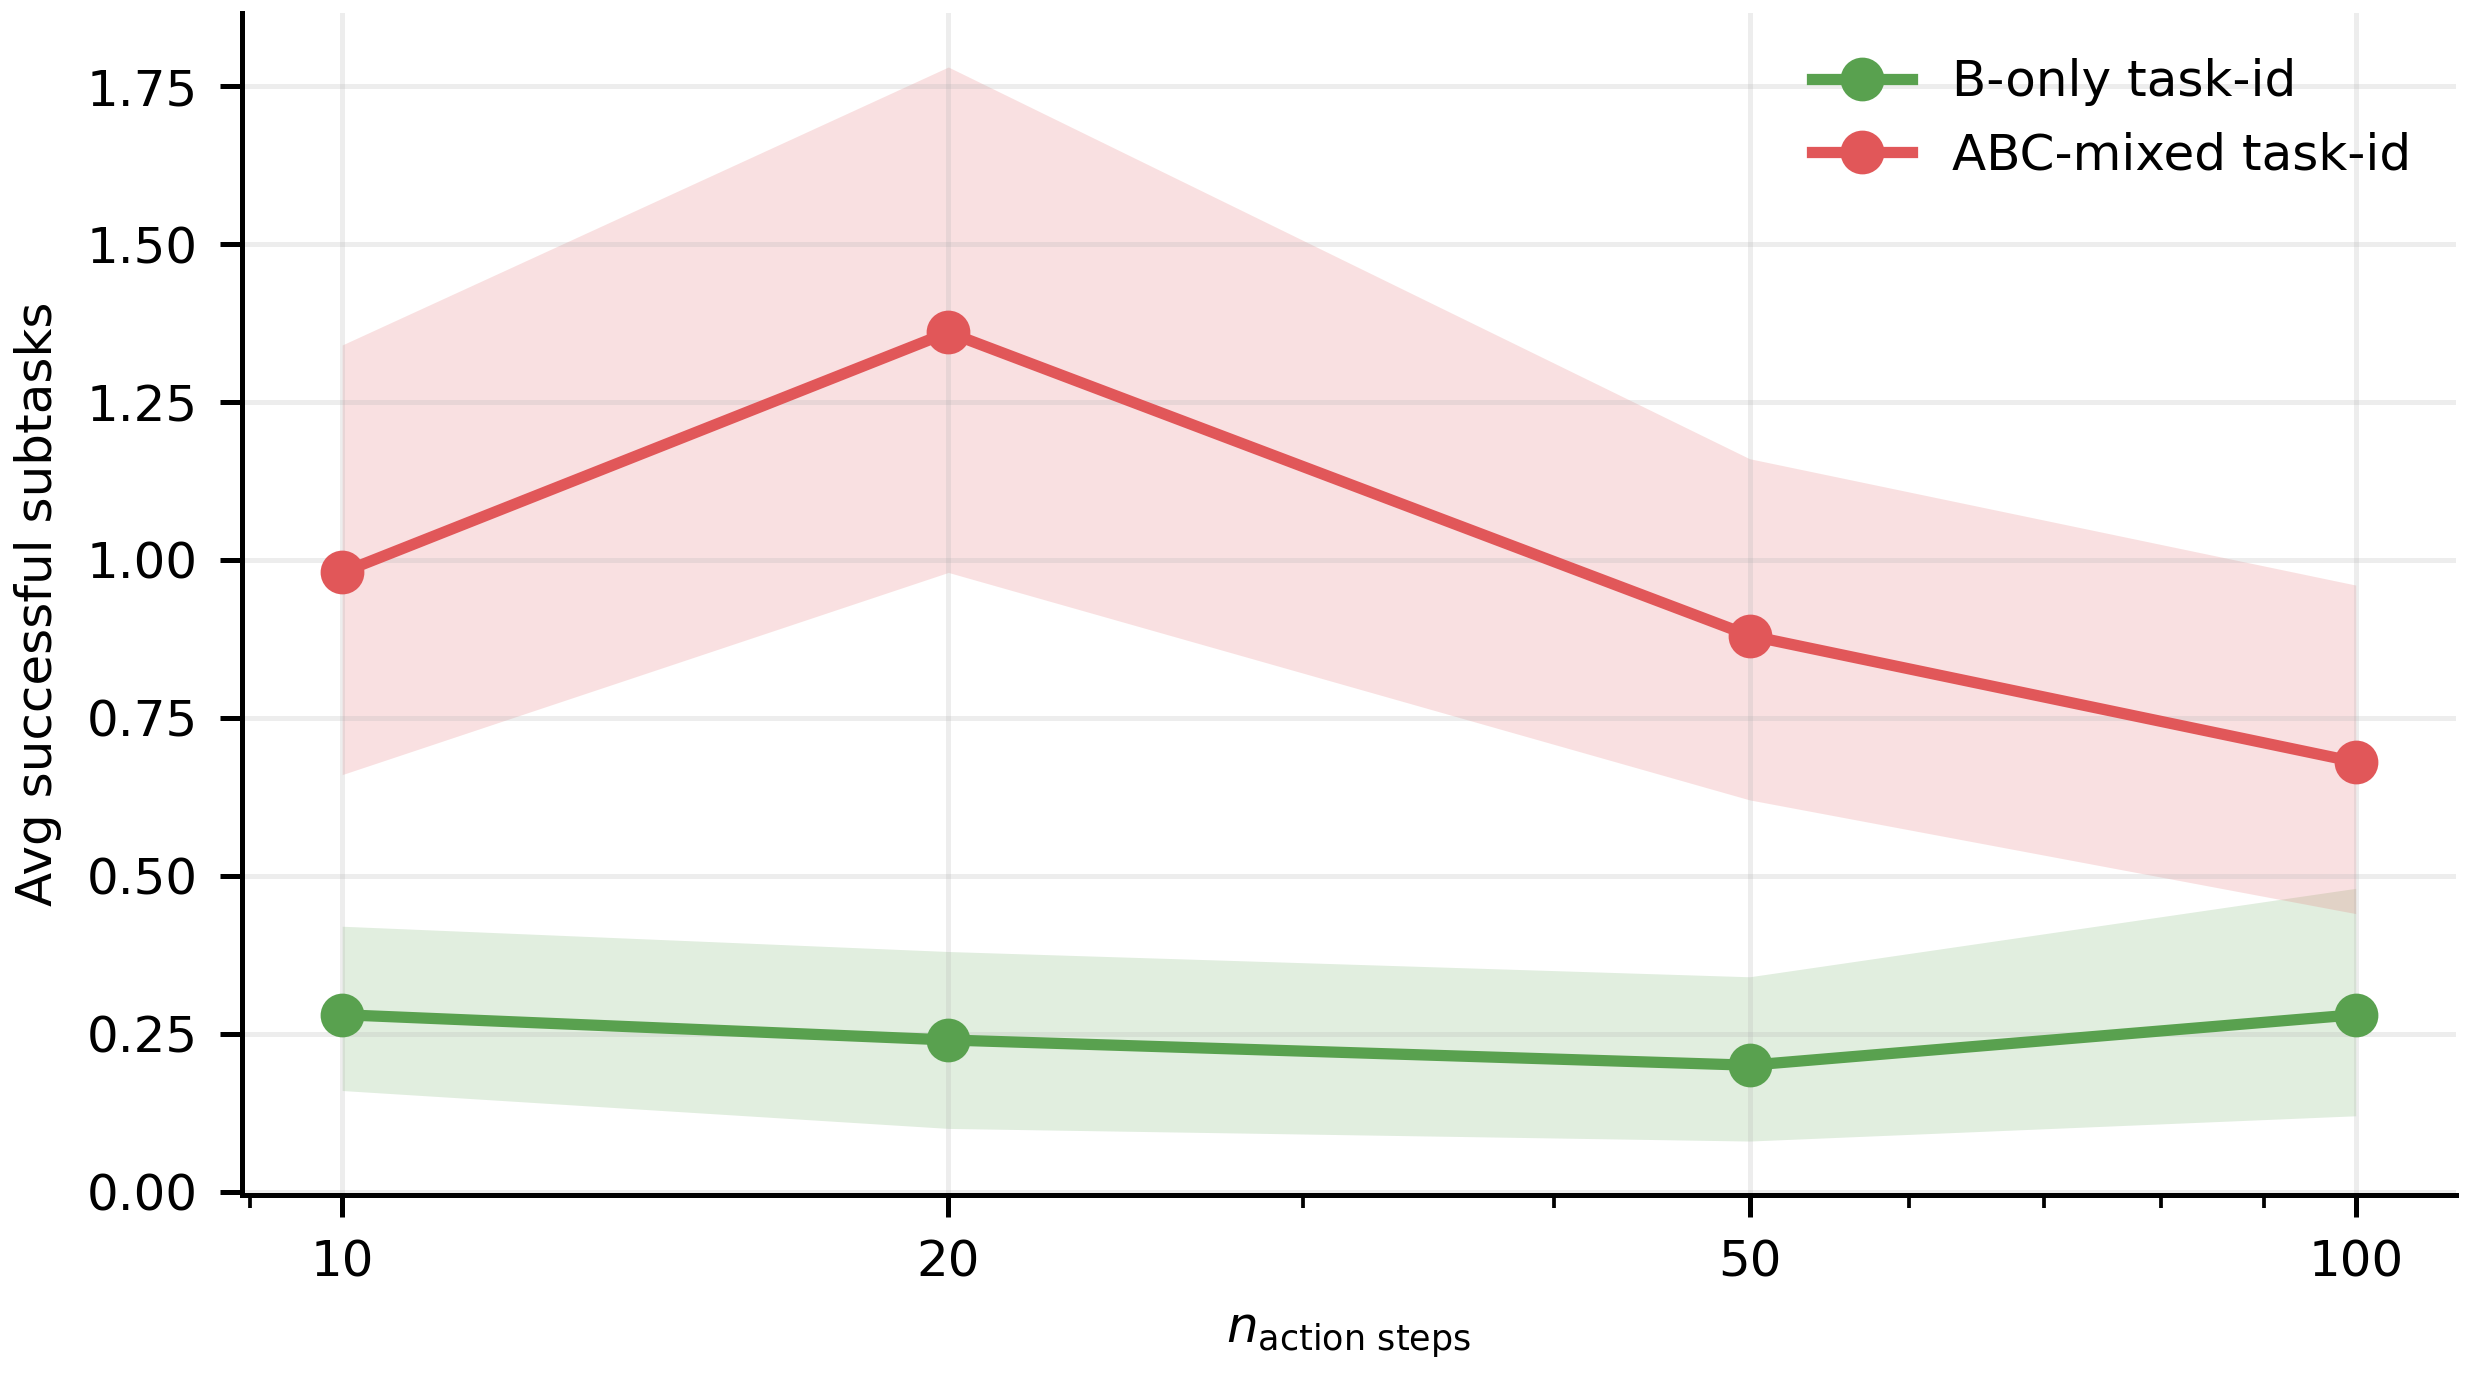
\includegraphics[width=0.72\linewidth]{../figures/track2_extra/extra1024_action_chunking_avg_success_ci.png}
\caption{Action chunking 消融的平均完成子任务数和 95\% bootstrap CI。训练 chunk size 固定为 100，只改变推理执行间隔。}
\label{fig:chunk_avg_ci}
\end{figure}

图~\ref{fig:chunk_rescue_waterfall} 逐序列比较 ABC-mixed task-id 的 $n=20$ 和 $n=100$。$n=20$ 在 21 条序列上完成更多子任务，22 条不变，7 条变差；seq\_08 和 seq\_44 都从 0/5 变为 5/5，seq\_22 从 1/5 变为 5/5。这个结果把平均值提升拆成具体样本：适度重规划能救回不少长链失败，但也会在少数序列上打断原本可行的动作块。

\begin{figure}[!htbp]
\centering
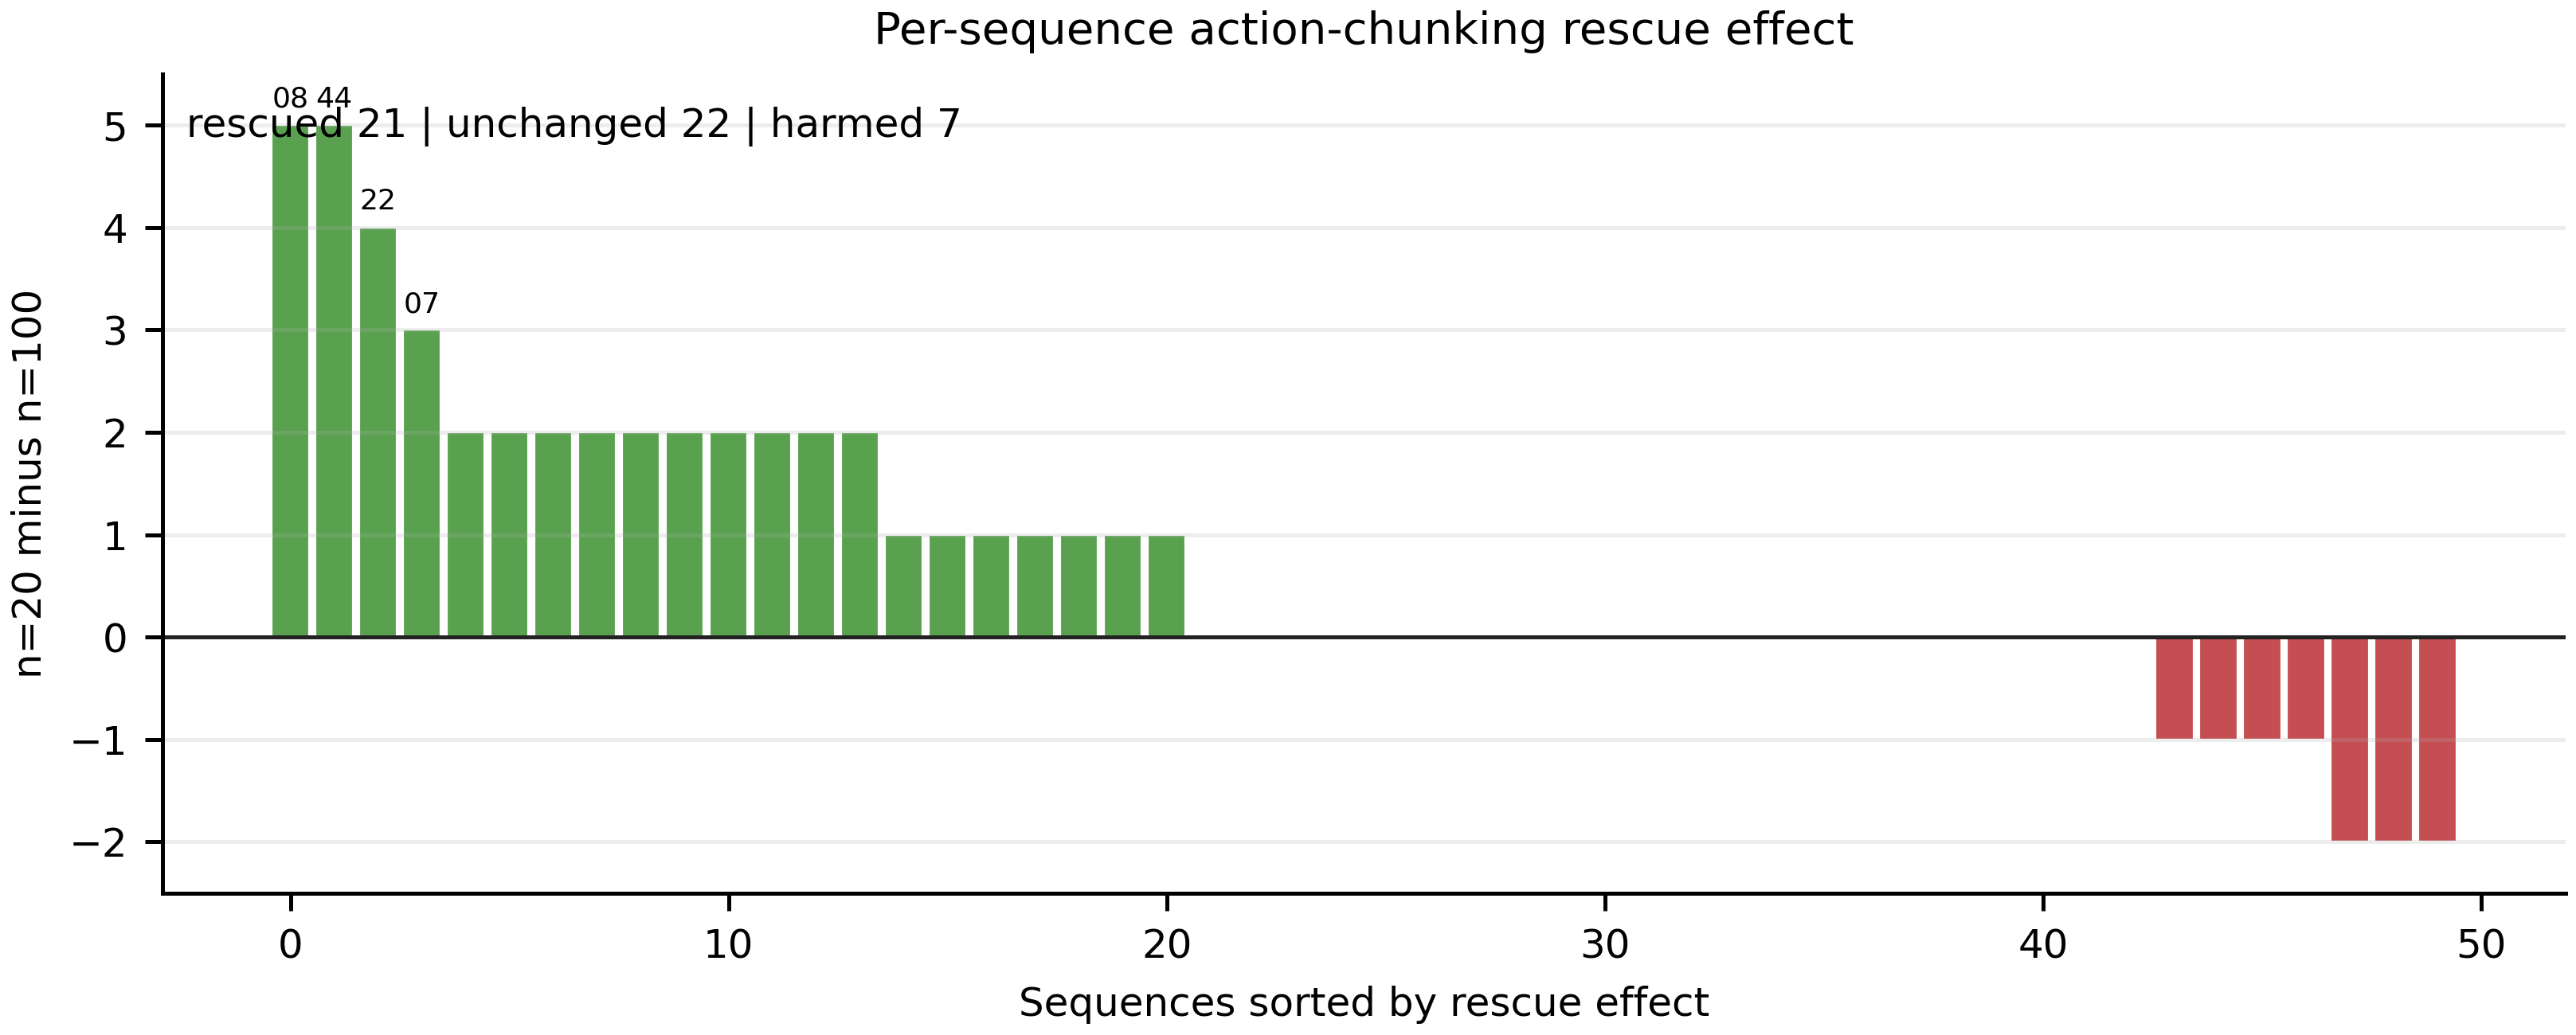
\includegraphics[width=0.86\linewidth]{../figures/track2_extra/extra1024_action_chunking_rescue_waterfall.png}
\caption{ABC-mixed task-id 的逐序列重规划收益。每根柱表示同一条序列上 $n=20$ 与 $n=100$ 的完成子任务数差值。}
\label{fig:chunk_rescue_waterfall}
\end{figure}

\begin{figure}[!htbp]
\centering
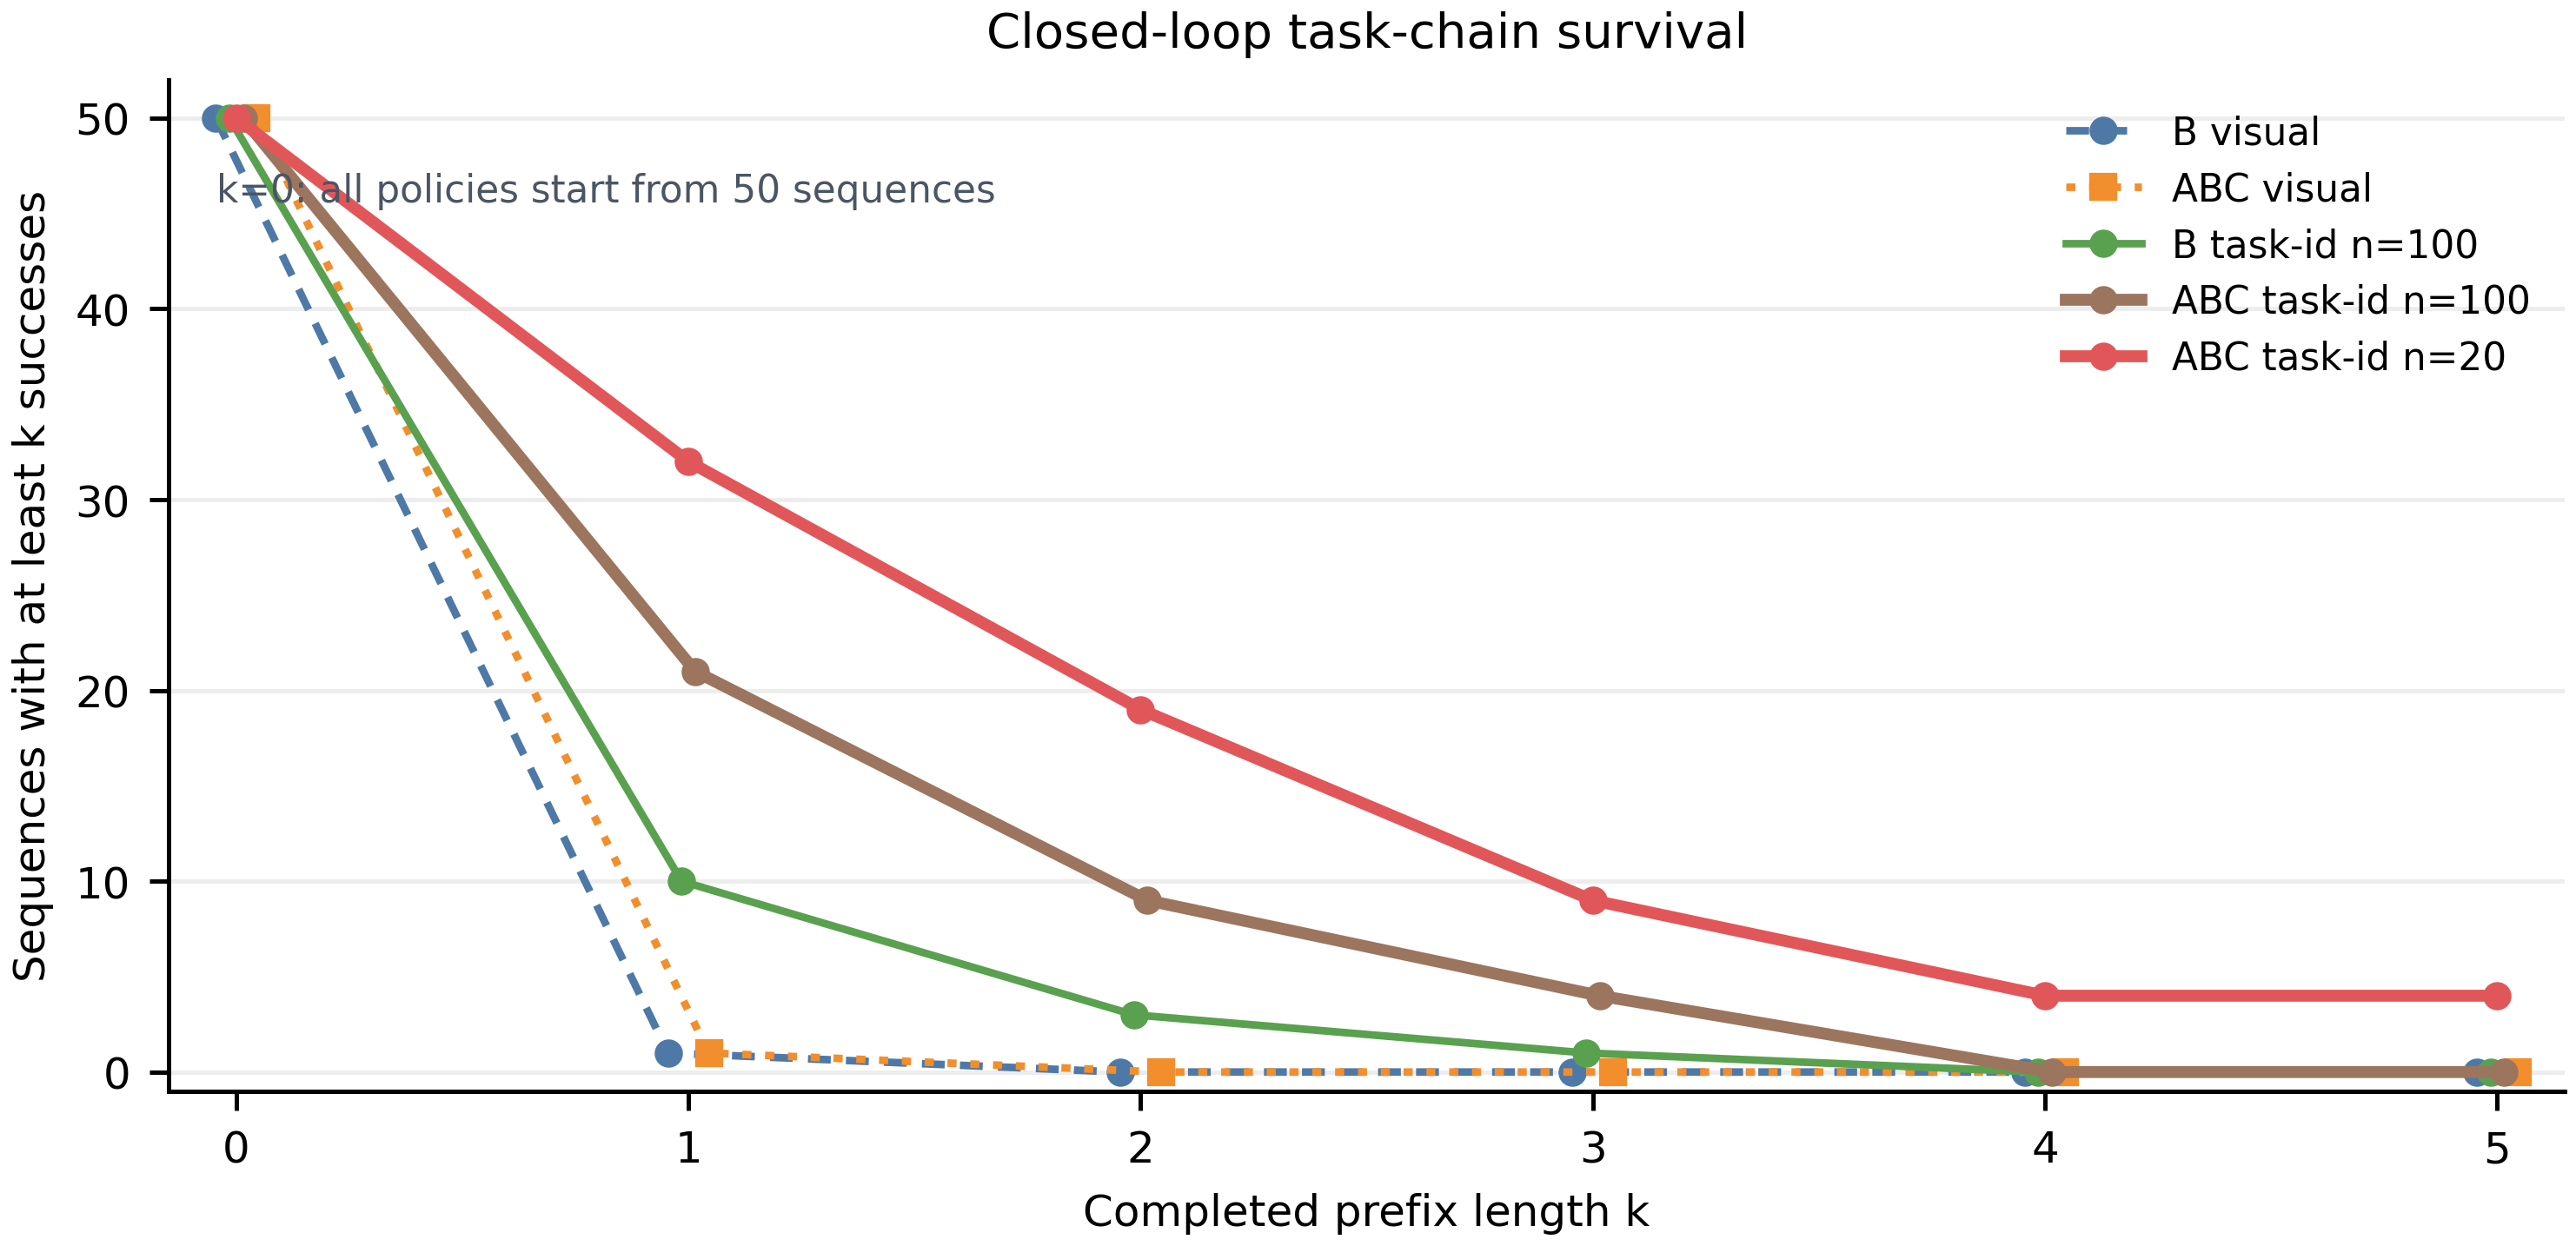
\includegraphics[width=0.82\linewidth]{../figures/track2_extra/extra1024_closed_loop_survival_curve.png}
\caption{闭环任务链存活曲线。纵轴为至少连续完成 $k$ 个子任务的序列数；$k=0$ 表示完成至少 0 个子任务，因此所有模型都从 50 条序列开始。B visual 与 ABC visual 高度重合，图中对 visual 曲线加入轻微横向偏移以便区分。}
\label{fig:sr_attrition}
\end{figure}

\begin{figure}[!htbp]
\centering
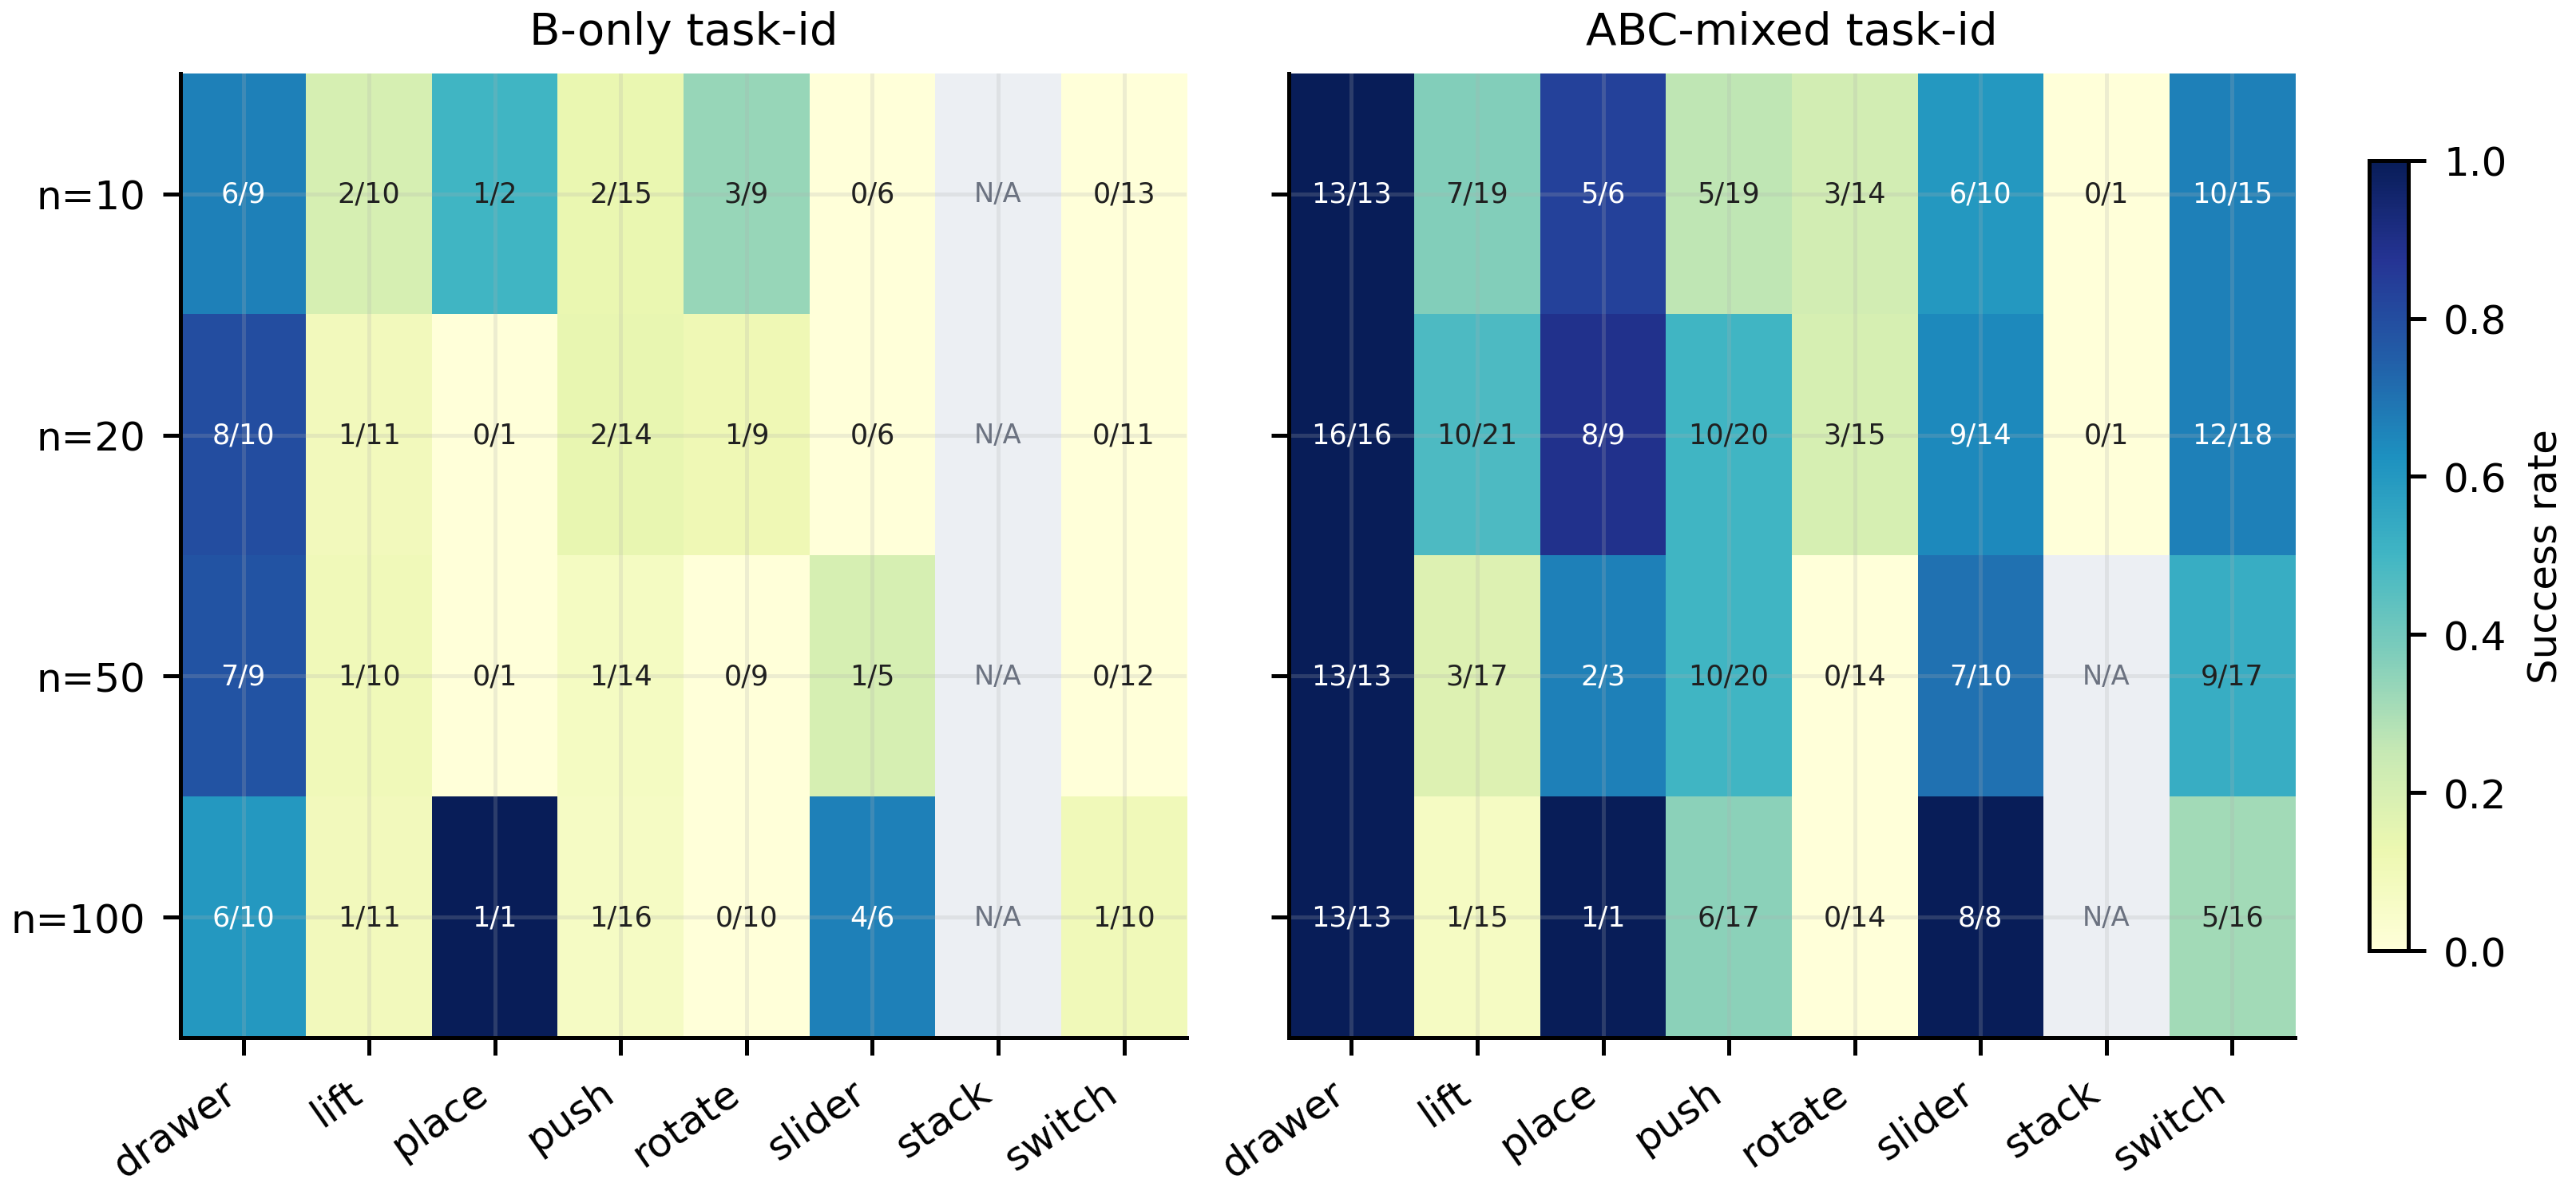
\includegraphics[width=\linewidth]{../figures/track2_extra/extra1024_action_chunking_task_family_heatmap.png}
\caption{重规划频率与 task family 的闭环成功率。每个格子的文字为成功数/尝试数，颜色为 success rate；N/A 表示该 family 在对应 rollout 中没有被执行到，不能解释为 0\% 成功率。}
\label{fig:chunk_family_heatmap}
\end{figure}

Task-family 热图把 $n=20$ 的收益定位到具体任务。ABC-mixed task-id 在 $n=20$ 下 drawer 为 16/16，place 为 8/9，slider 为 9/14，push 为 10/20；$n=100$ 下 lift 从 10/21 降到 1/15，rotate 从 3/15 降到 0/14，switch 从 12/18 降到 5/16。完成子任务数直方图也呈现同样结构：ABC-mixed task-id 在 $n=20$ 下有 4 条序列完成 5/5，$n=100$ 下没有序列达到 5/5；$n=100$ 的 0-completed 序列为 29 条，$n=20$ 降到 18 条。

图~\ref{fig:family_position_matrix} 继续把 task family 拆到链条位置。每个格子只统计实际尝试过的子任务，前序失败导致的未尝试位置标为 N/A，不按失败计。$n=20$ 对 drawer、slider 和 place 的成功率稳定，push 在第 1 个子任务位置有 8/13 成功；rotate 在 $n=100$ 下所有尝试位置均为 0 成功，$n=20$ 仍然较弱但不再全零。该矩阵显示，重规划主要改善需要反馈修正的推、拉、放置任务，姿态旋转仍是主要瓶颈。

\begin{figure}[!htbp]
\centering
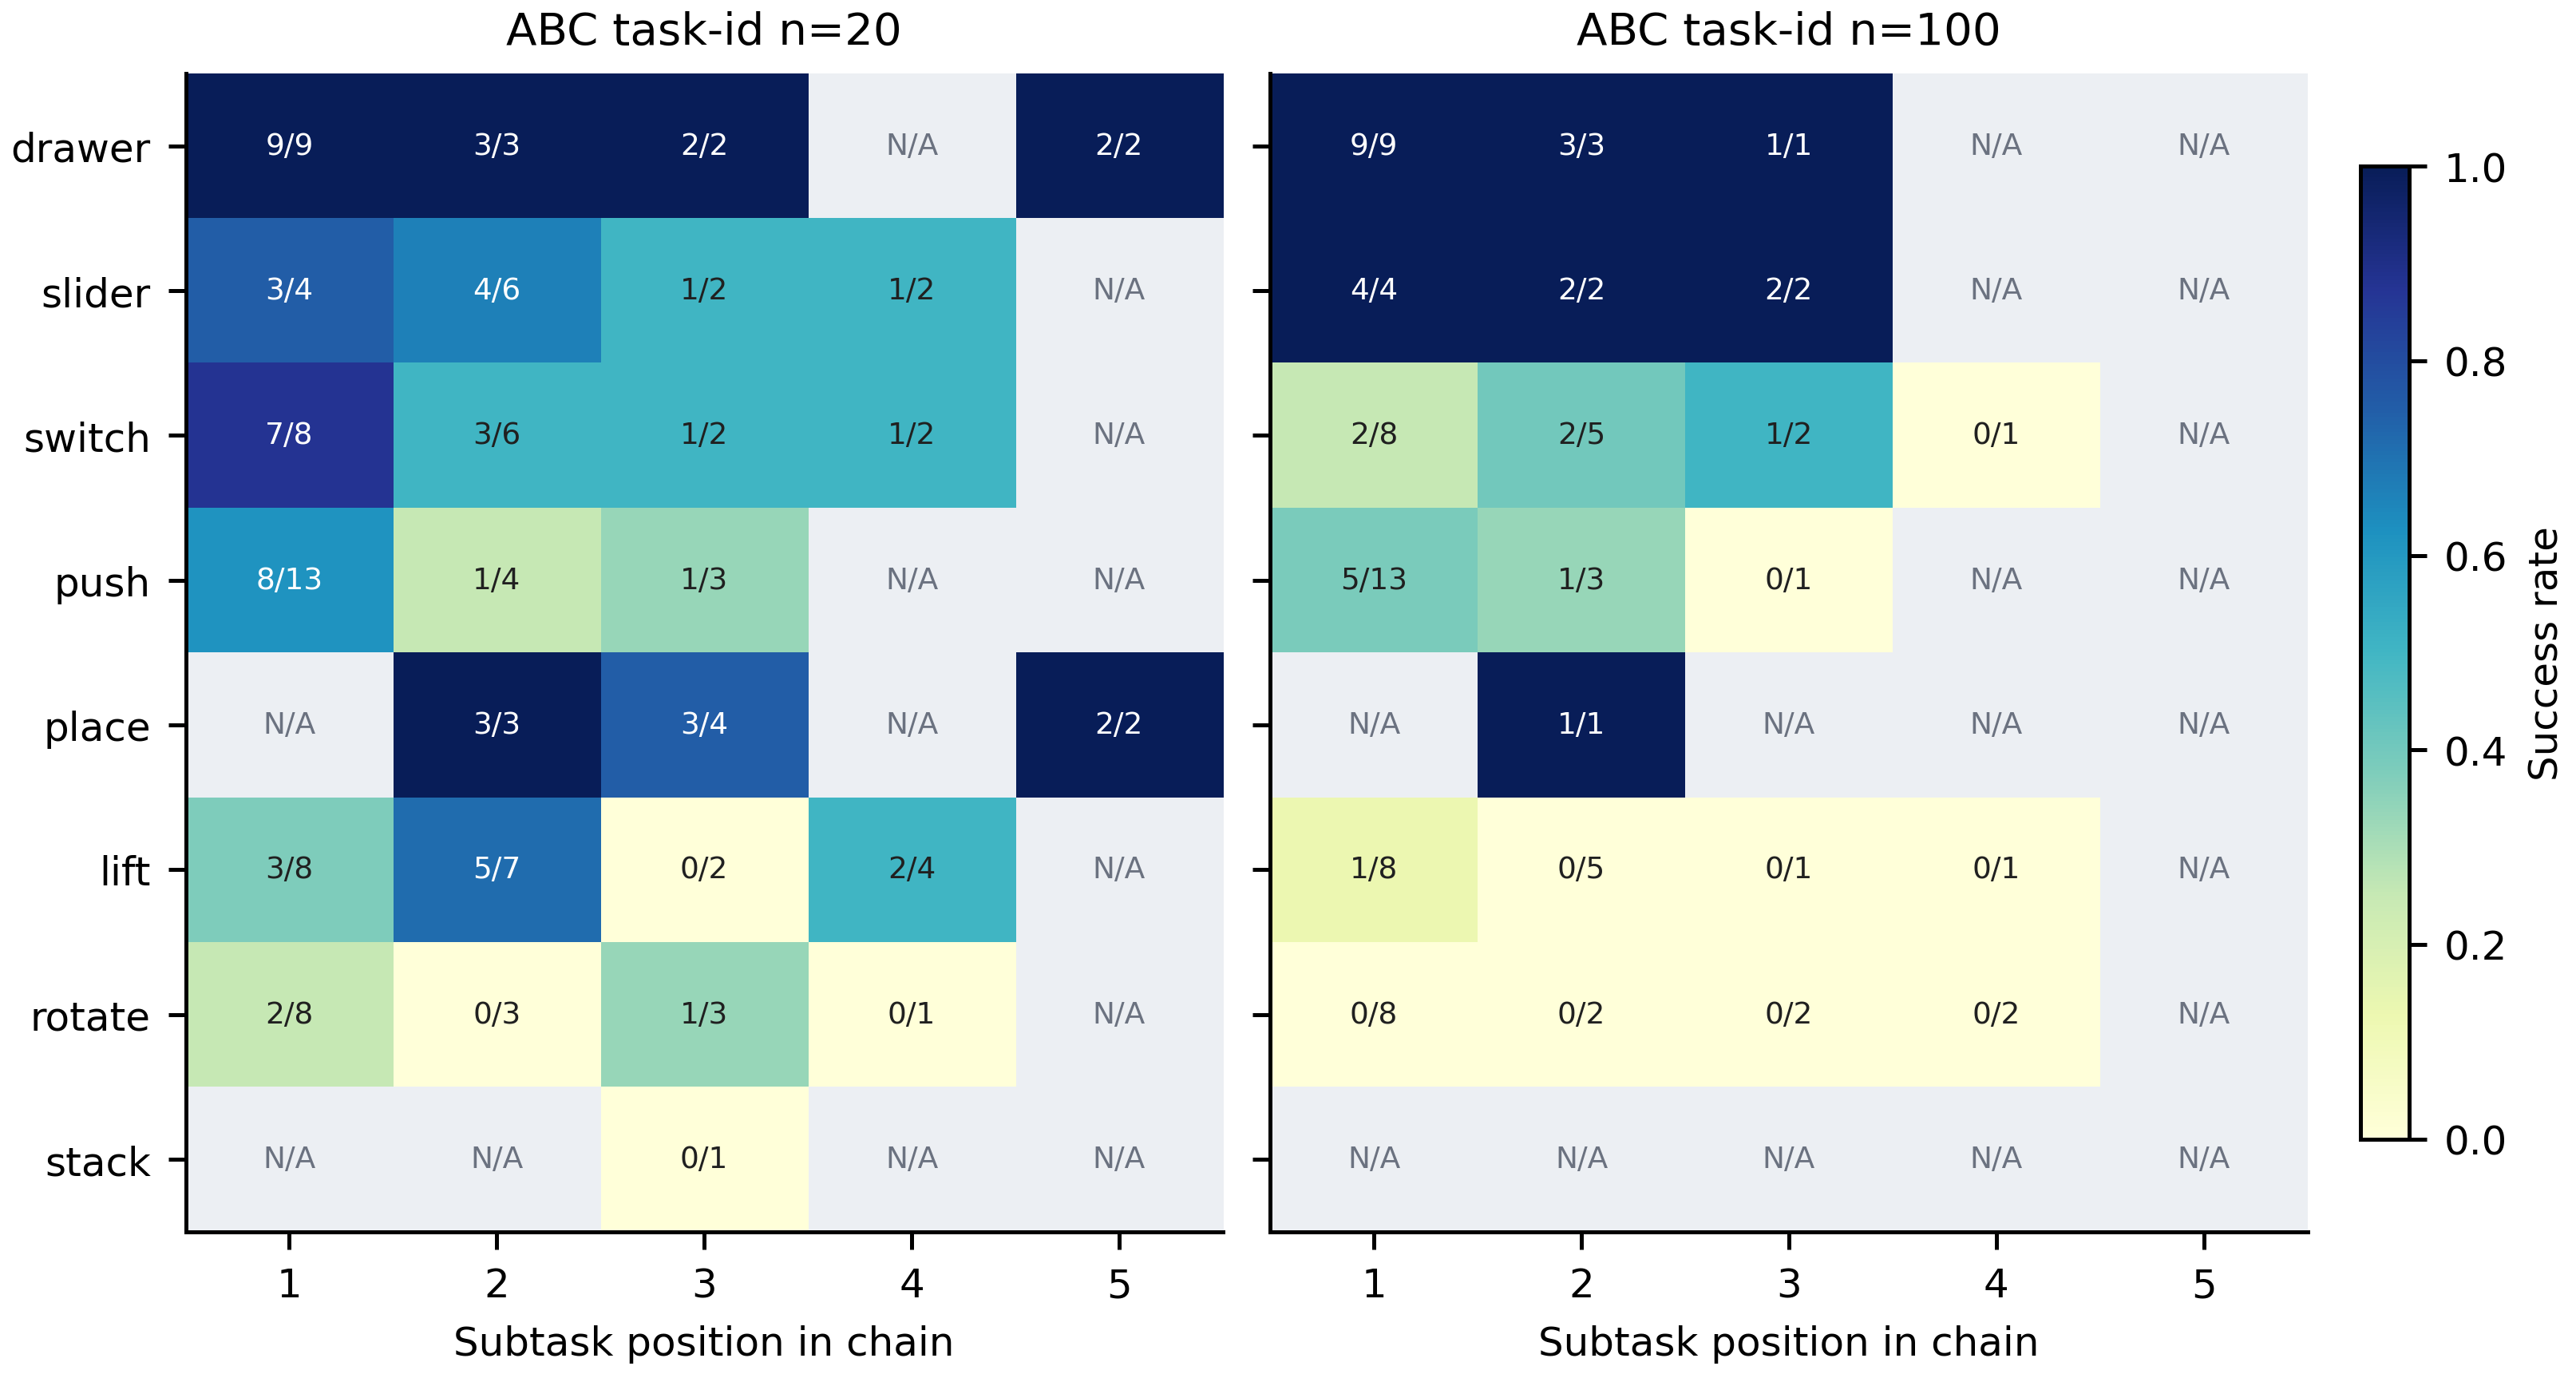
\includegraphics[width=\linewidth]{../figures/track2_extra/extra1024_action_chunking_task_family_position_matrix.png}
\caption{ABC-mixed task-id 的 task family $\times$ 链条位置成功率。文字为成功数/尝试数；N/A 表示该位置没有被执行到。}
\label{fig:family_position_matrix}
\end{figure}

\begin{figure}[!htbp]
\centering
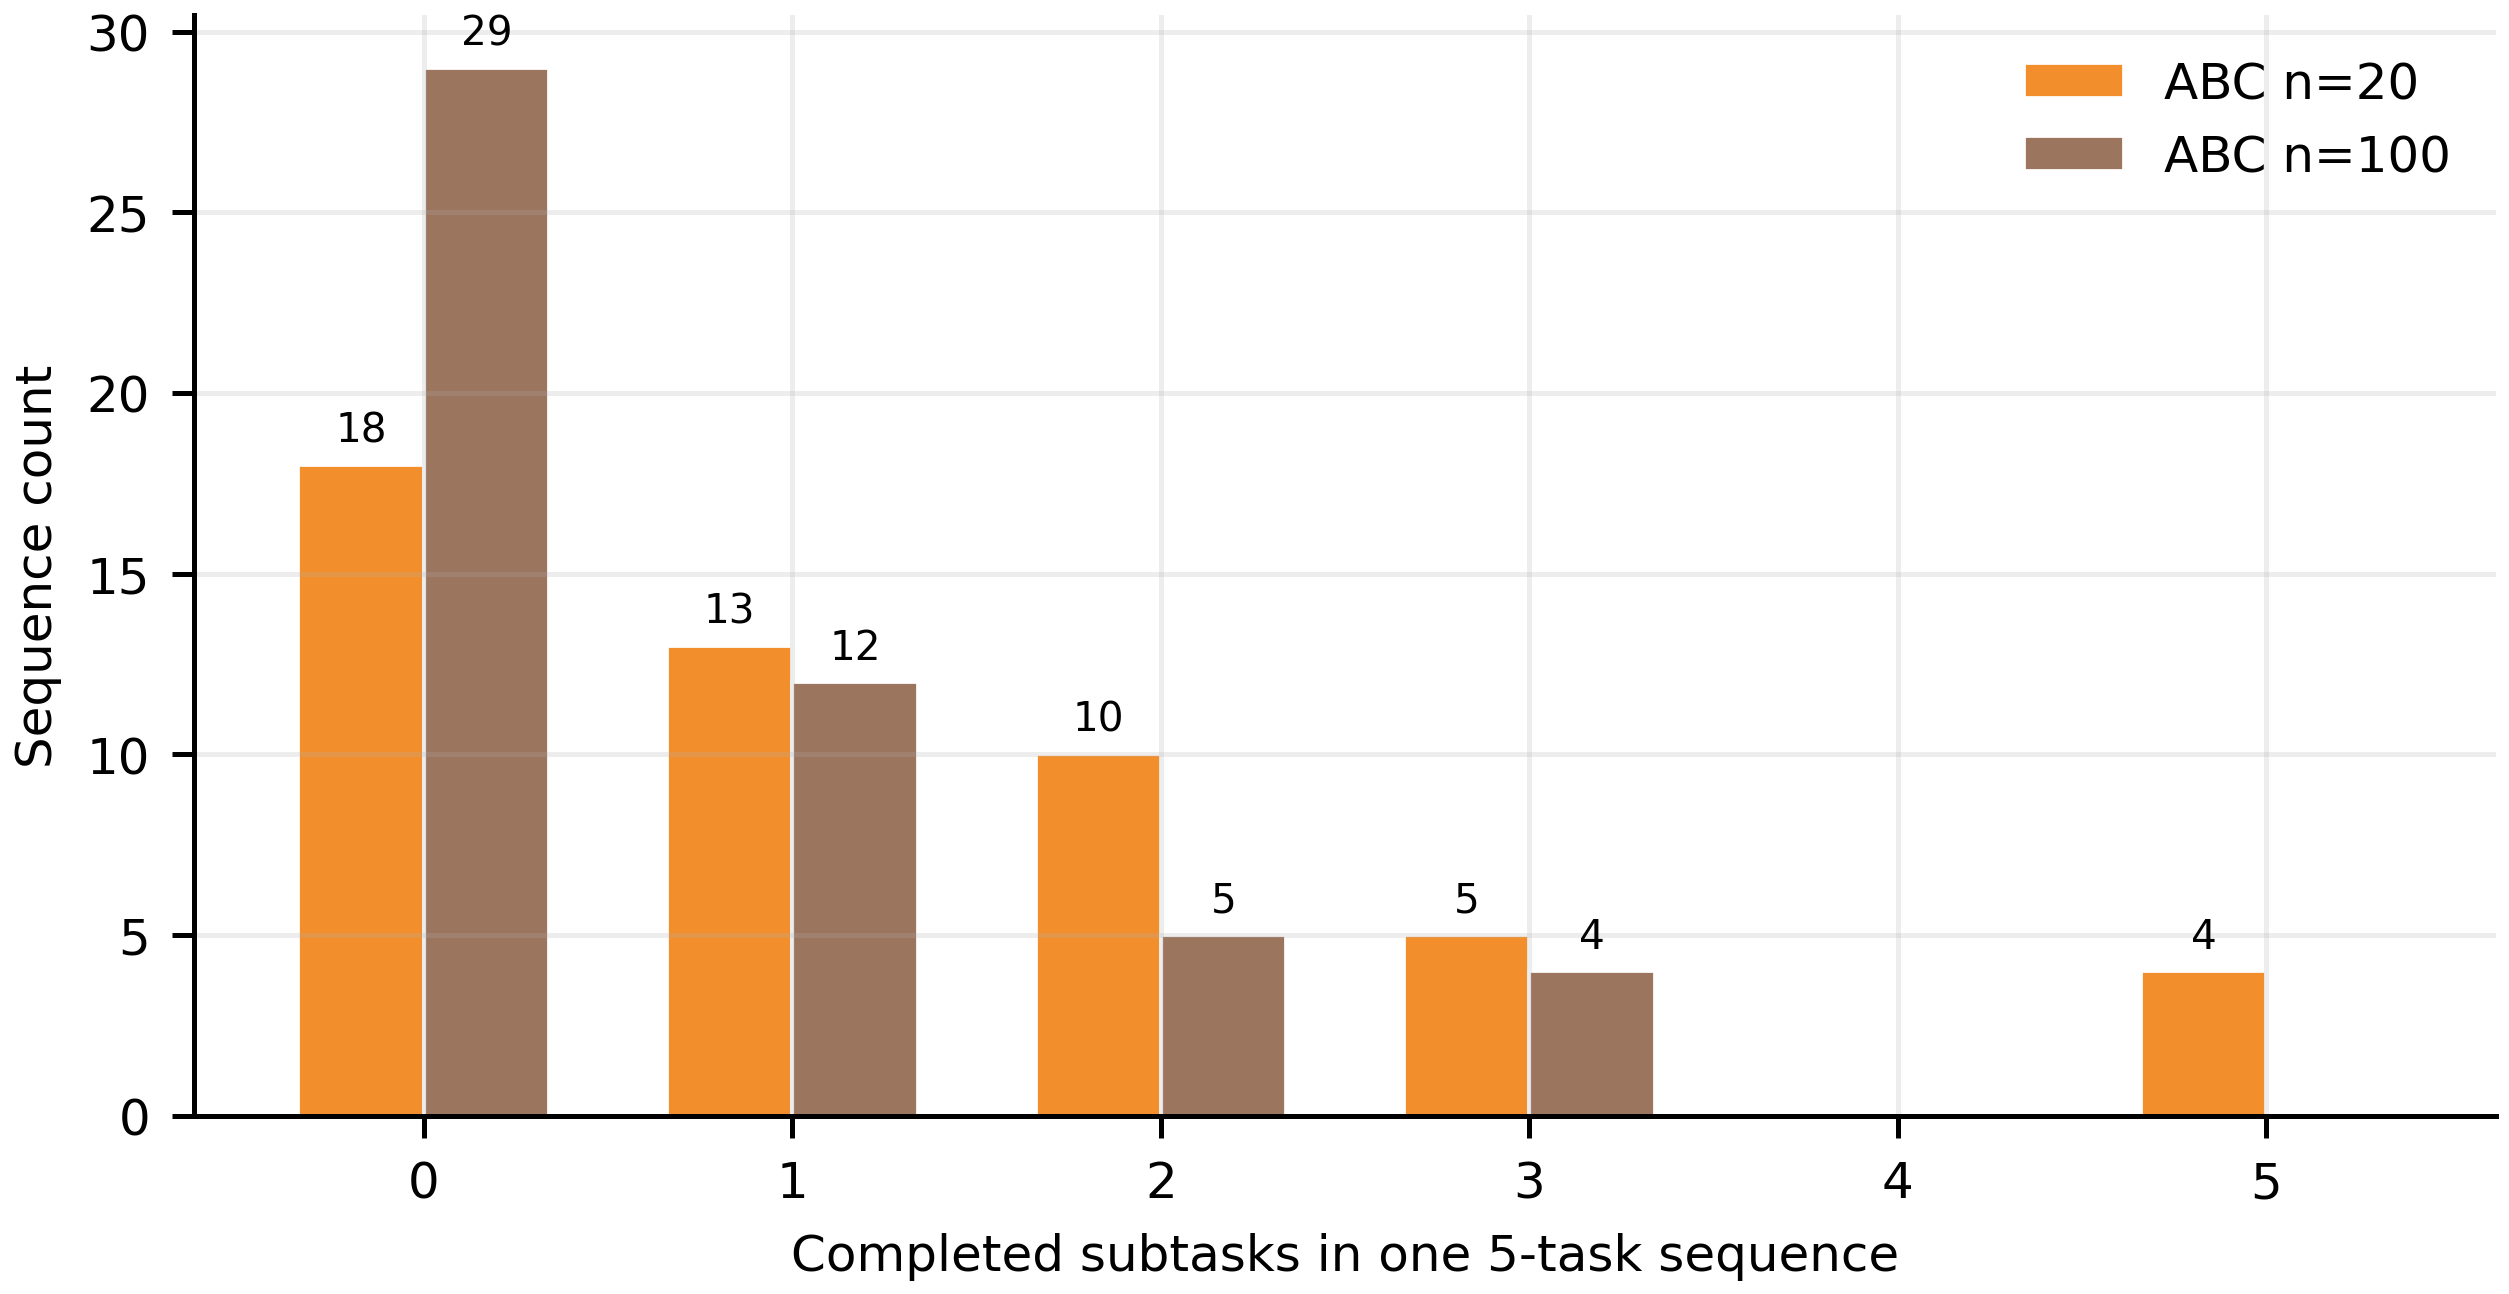
\includegraphics[width=0.70\linewidth]{../figures/track2_extra/extra1024_action_chunking_completed_hist_abc_n20_n100.png}
\caption{ABC-mixed task-id 在 $n=20$ 和 $n=100$ 下的 completed-subtasks 分布。横轴为单条 5-task 序列中完成的子任务个数。}
\label{fig:chunk_completed_hist}
\end{figure}

\begin{figure}[!htbp]
\centering
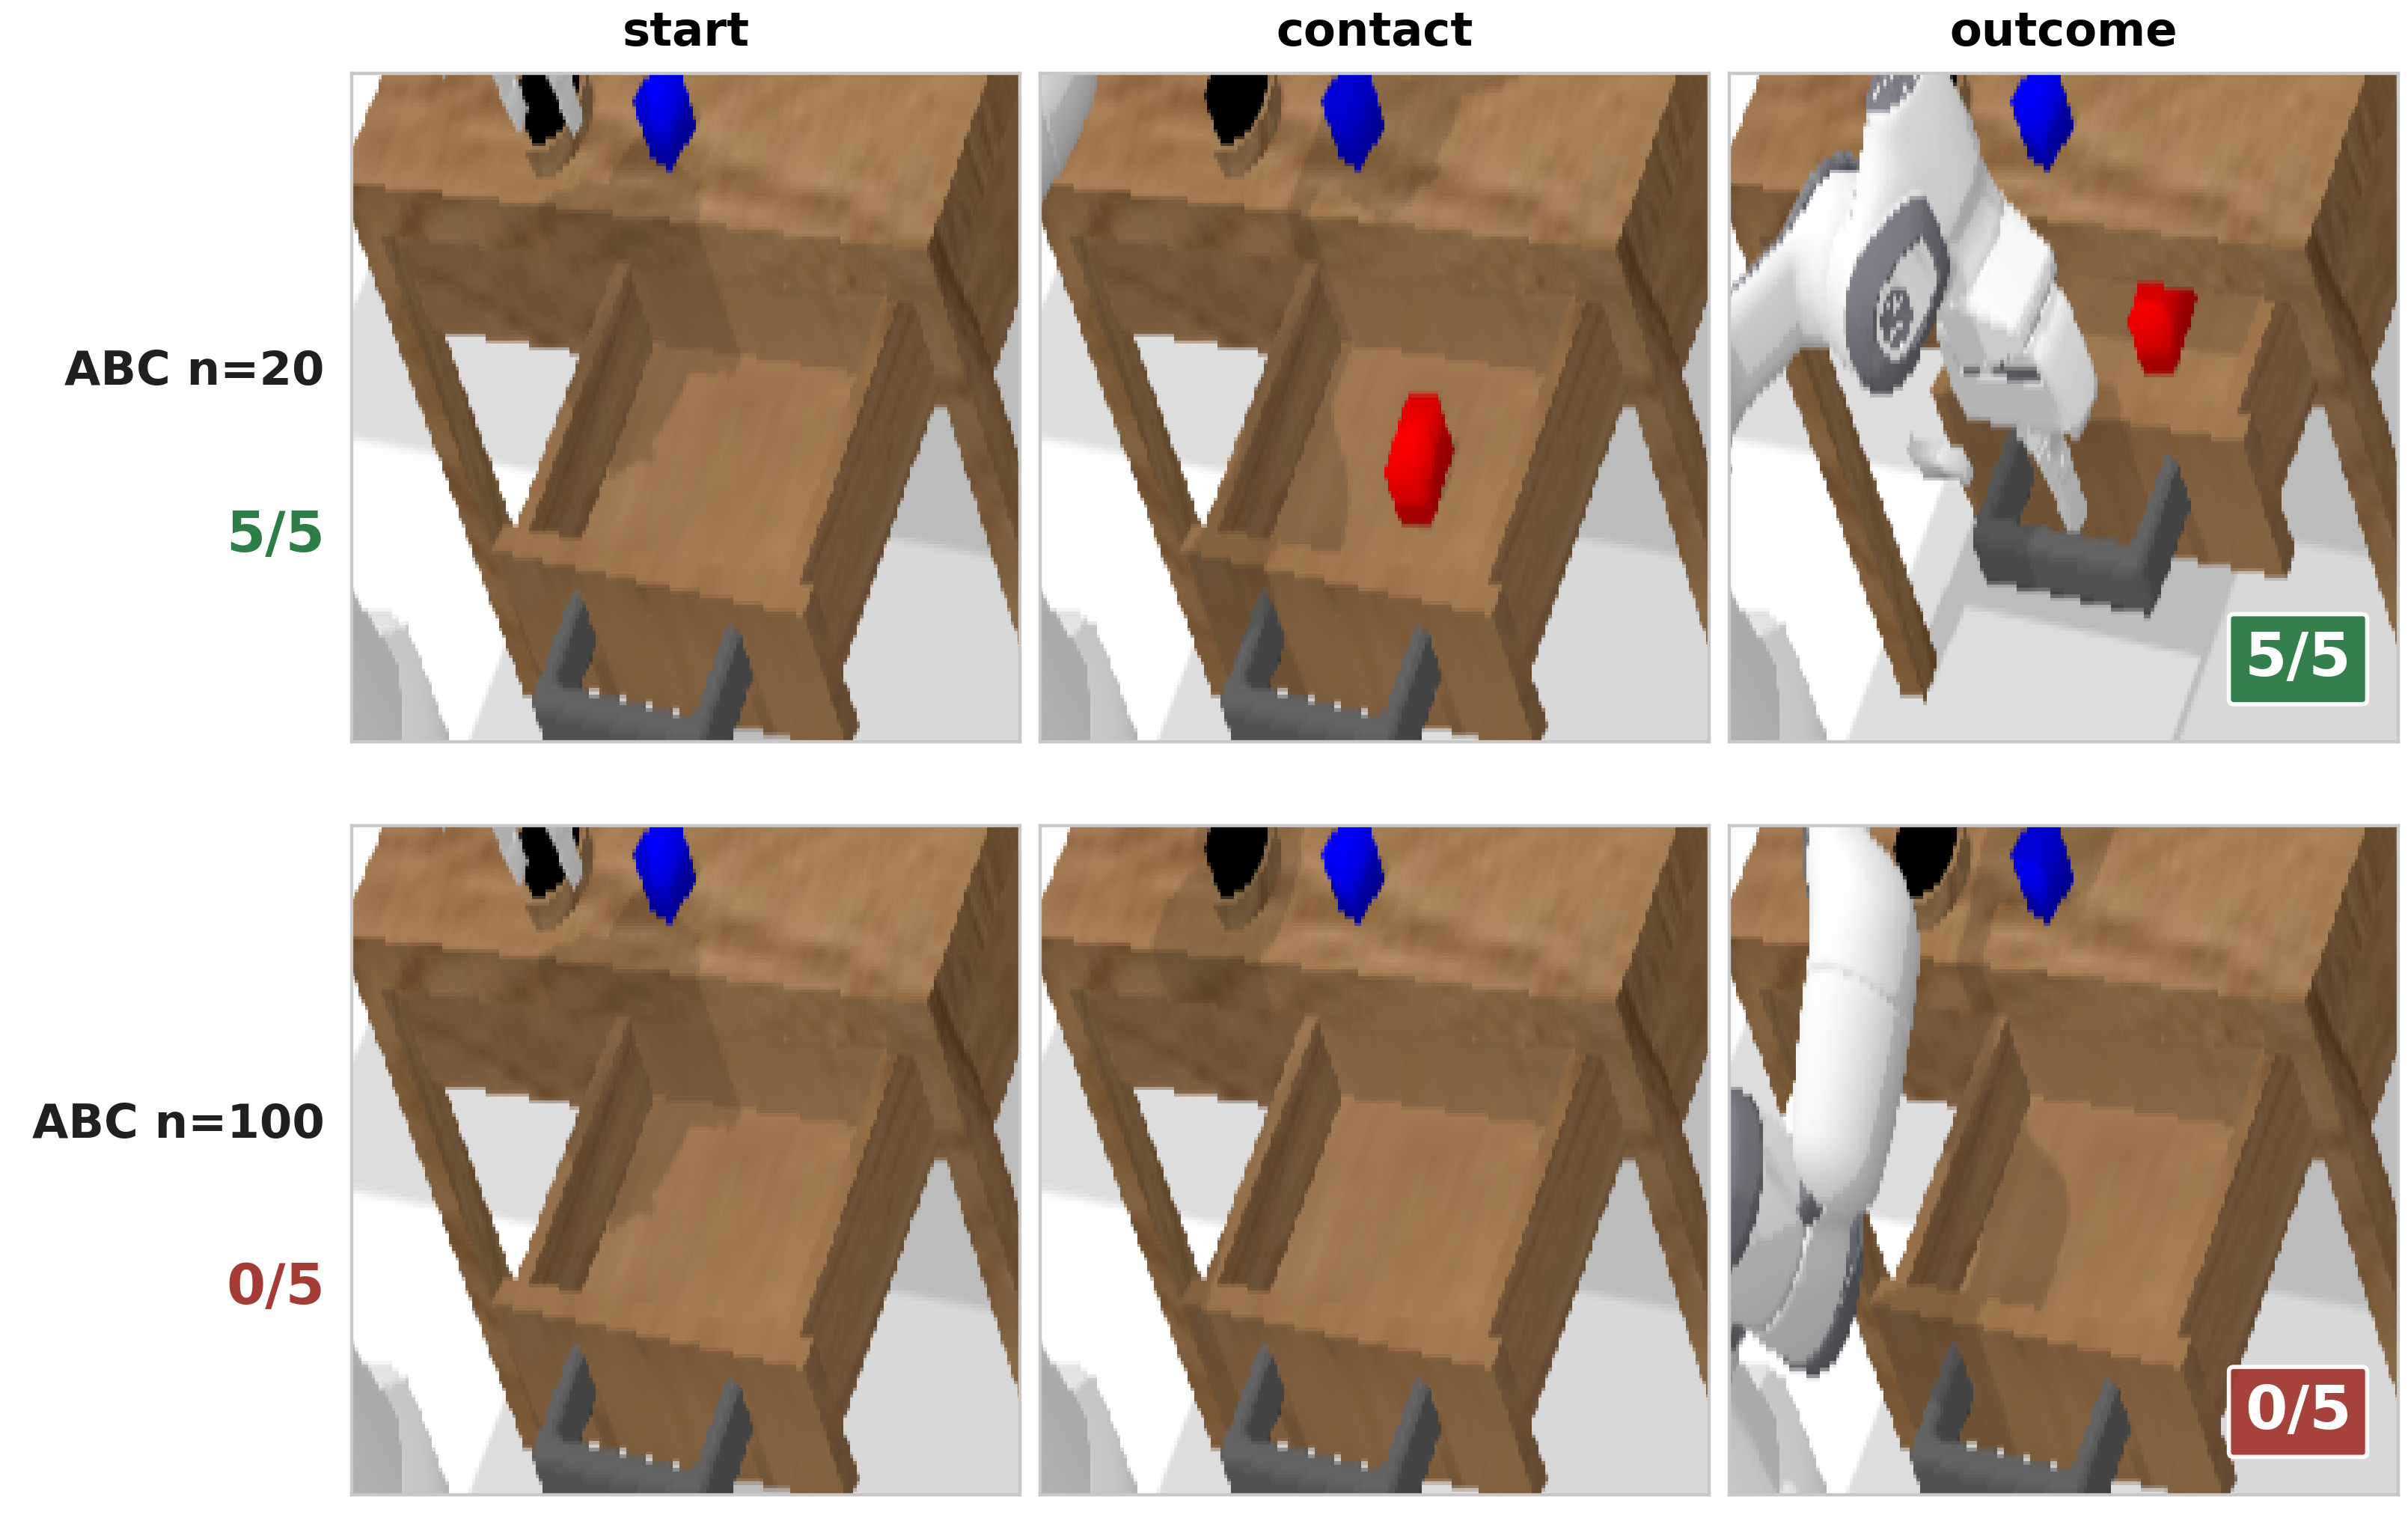
\includegraphics[width=\linewidth]{../figures/track2_extra/rollout_seq08_action_chunking_keyframes.png}
\caption{ABC-mixed task-id 在 seq\_08 上的 $n=20$ 与 $n=100$ 关键帧对比。两行使用相同初始状态和任务链；$n=20$ 完成 5/5，$n=100$ 停在 0/5。}
\label{fig:chunk_qual}
\end{figure}

这些结果解释了为什么“预测 100 步、执行 20 步后重新预测”优于把动作块缩短为只预测 20 步。训练时的 100-step chunk 保留了长接触轨迹和动作连续性；推理时的 20-step execution interval 让模型更早看到抽屉是否移动、滑块是否到位、方块是否偏离。$n=10$ 低于 $n=20$，说明过短间隔会打断 ACT 学到的连续动作。D 环境中的鲁棒性来自多源视觉覆盖和适度重规划的配合。

\FloatBarrier

\subsection{Task-id 诊断与失败模式}

task-id 扩展把语言目标写入低维条件向量。为检查模型是否真的使用任务条件，我们在 D-1024 offline 上固定图像和机器人状态，只替换 task id：correct、zero、random、same-family wrong 和 different-family wrong。该诊断不改变视觉输入，专门测任务条件对动作预测的控制作用。

\begin{table}[!htbp]
\centering
\scriptsize
\caption{D-1024 task-id ablation。Same-fam. 和 Diff-fam. 分别表示同族错误 task id 和异族错误 task id；括号中为相对 correct 的 normalized \actionlone{} 增量比例。}
\label{tab:taskid_family_ablation}
\begin{tabular}{@{}lccccc@{}}
\toprule
模型 & Correct & Zero & Random & Same-fam. & Diff-fam. \\
\midrule
B-only & 0.615 & 0.753 (+22.4\%) & 0.712 (+15.9\%) & 0.717 (+16.7\%) & 0.720 (+17.1\%) \\
ABC-mixed & \best{0.507} & 0.843 (+66.3\%) & 0.759 (+49.6\%) & 0.782 (+54.2\%) & 0.765 (+50.8\%) \\
\bottomrule
\end{tabular}
\end{table}

表~\ref{tab:taskid_family_ablation} 中，正确 task id 始终给出最低误差。ABC-mixed task-id 对任务条件更敏感：清零 task id 后 normalized \actionlone{} 从 0.507 升到 0.843；随机 task id、同族错误 task id 和异族错误 task id 也都落在 0.759--0.782。B-only task-id 的同类退化为 15.9\%--22.4\%。同族错误没有恢复正确动作，表明模型使用的是具体任务目标，而非只使用 ``push/lift/rotate'' 这一类粗粒度标签。

\begin{figure}[!htbp]
\centering
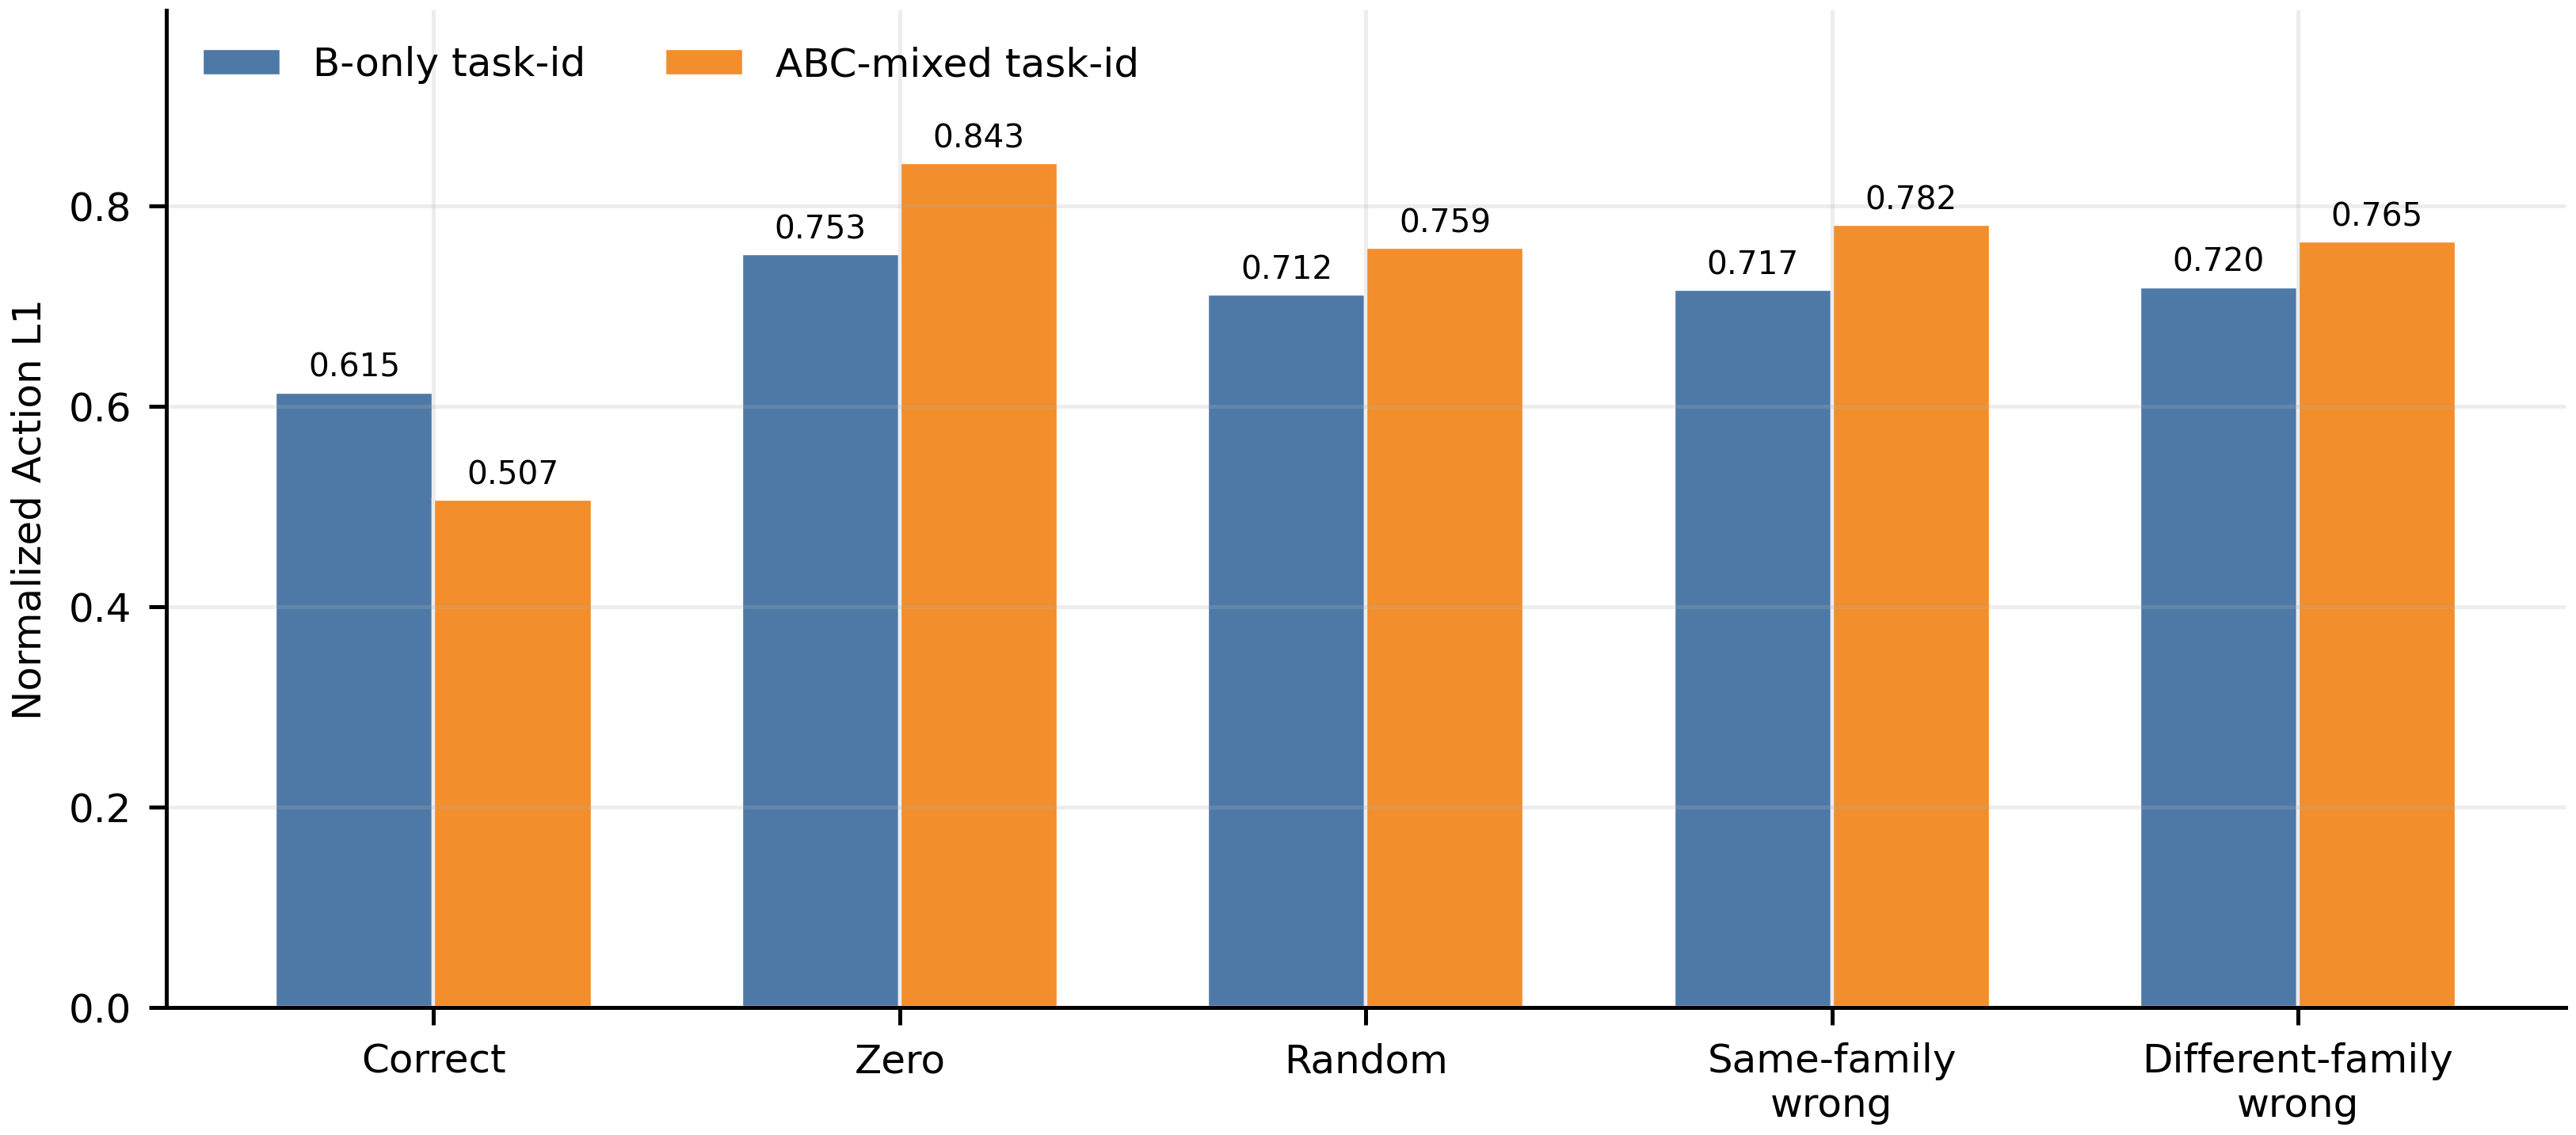
\includegraphics[width=0.86\linewidth]{../figures/track2_extra/extra1024_taskid_ablation_summary.png}
\caption{D-1024 task-id ablation。图像输入和机器人状态固定，只替换 task id。}
\label{fig:taskid_family_ablation}
\end{figure}

动作维度 gain 把 task-id 的作用落到具体控制量上。图~\ref{fig:action_dim_gain} 以 normalized \actionlone{} reduction 为颜色，正值表示改动降低误差。ABC-mixed visual 相对 B-only visual 在 gripper 上降低 0.19，在 $y$ 和 $z$ 上分别降低 0.11 和 0.10；ABC-mixed task-id 相对 ABC-mixed visual 在 yaw 上再降低 0.17，在 $x$ 和 $y$ 上各降低约 0.08--0.10。B-only visual 与 ABC-mixed task-id 的直接差值集中在 gripper、yaw、$y$、$x$ 和 $z$；roll 基本没有改善。

\begin{figure}[!htbp]
\centering
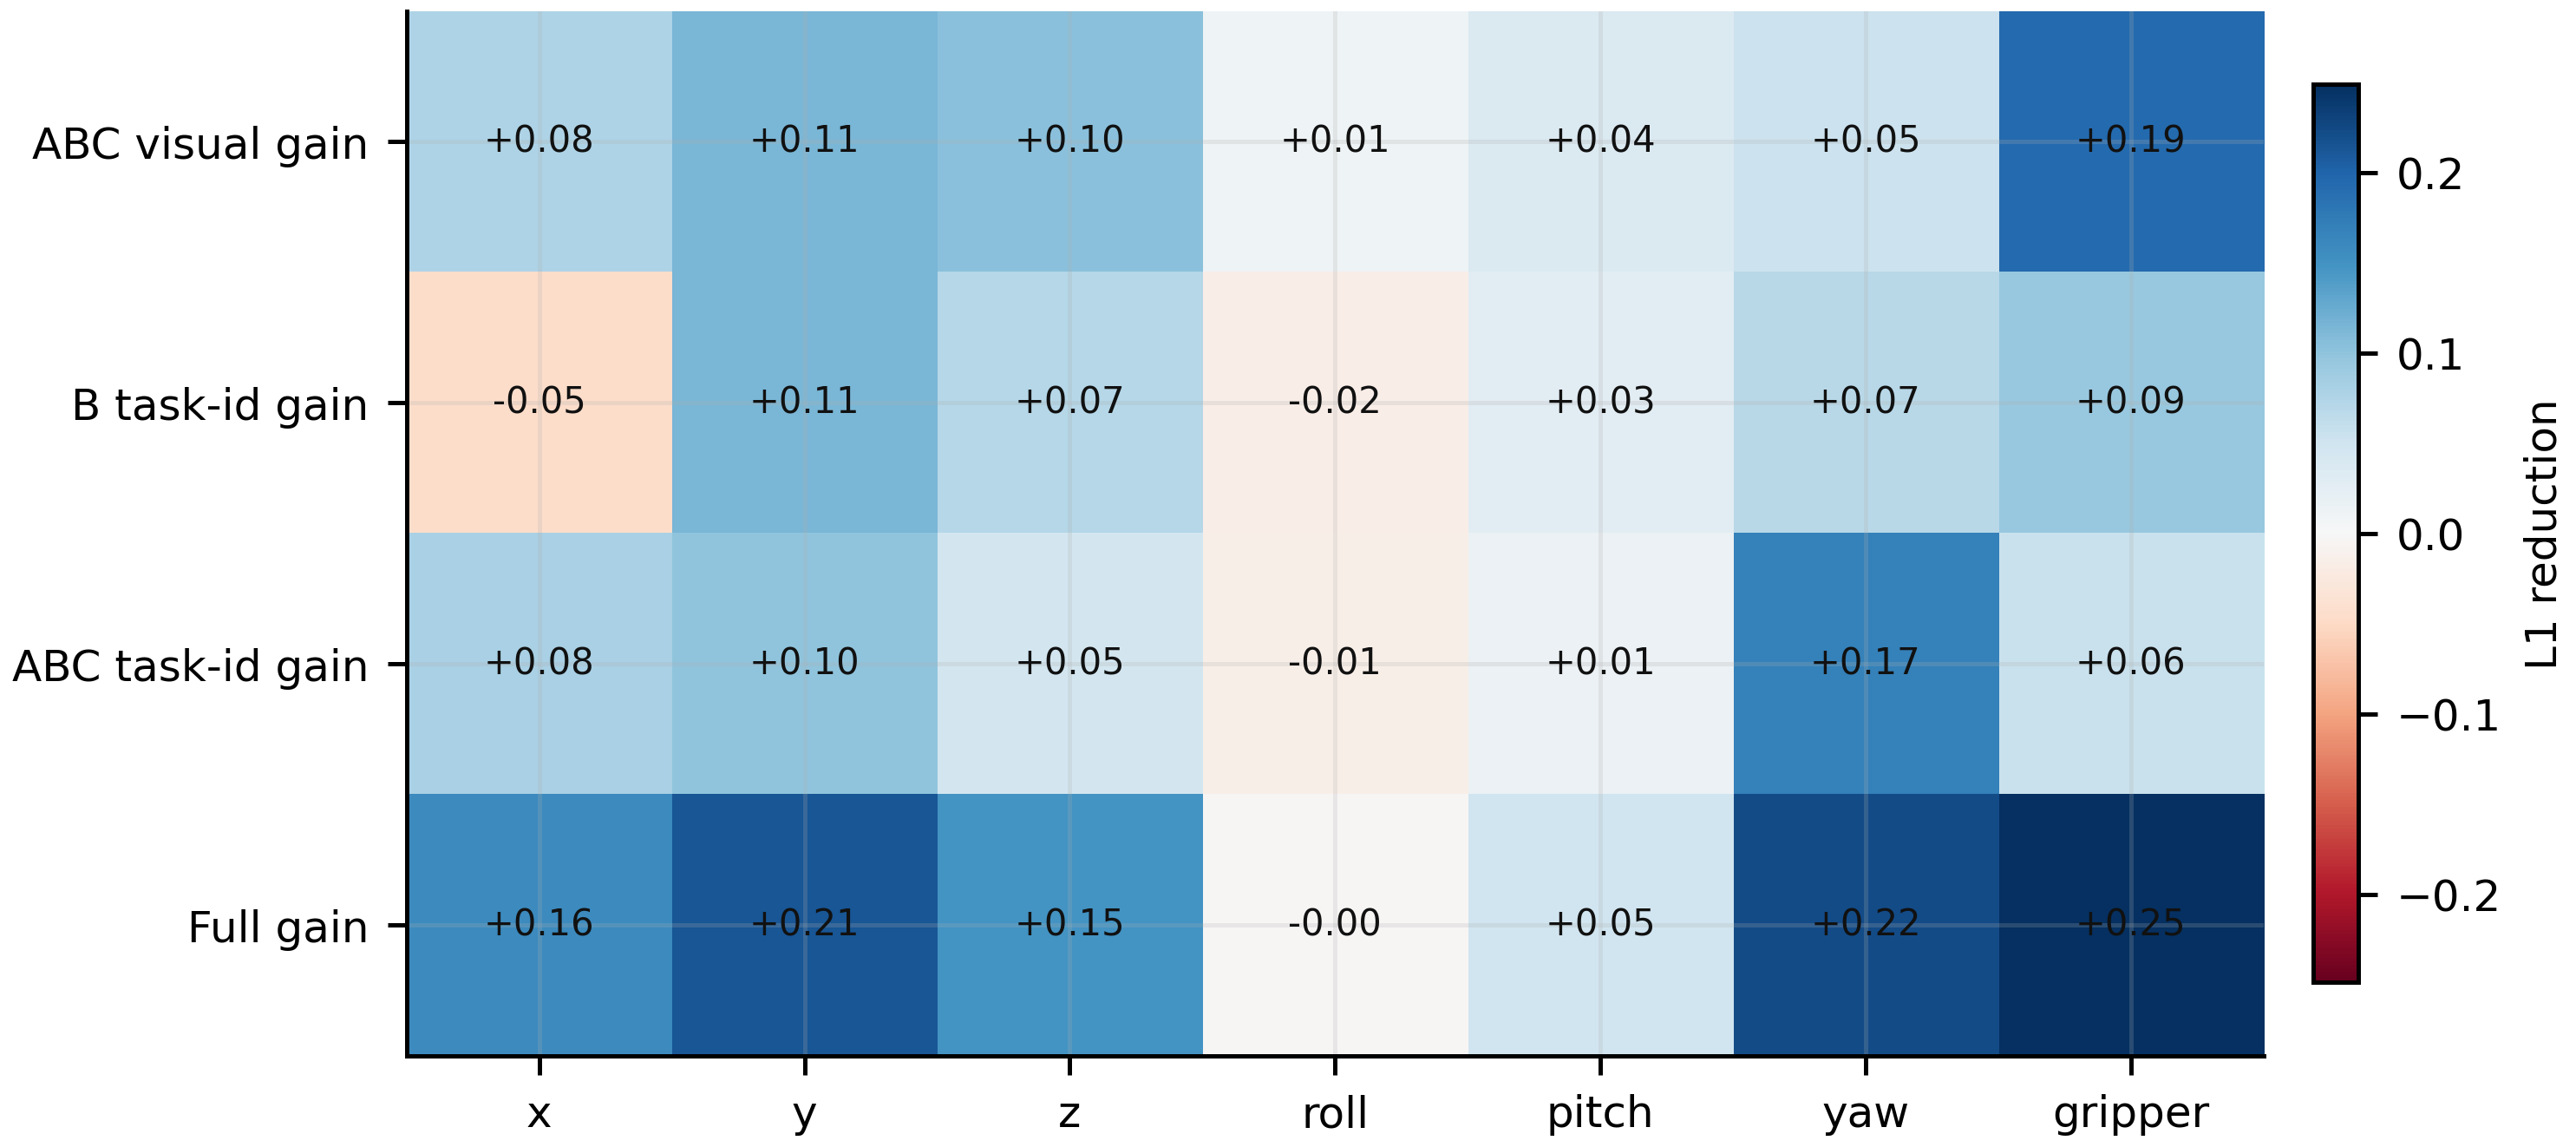
\includegraphics[width=0.84\linewidth]{../figures/track2_extra/extra1024_action_dim_gain_heatmap.png}
\caption{动作维度上的 normalized \actionlone{} reduction。蓝色表示误差下降，红色表示误差上升。}
\label{fig:action_dim_gain}
\end{figure}

剩余失败集中在对姿态和接触更敏感的任务。task-family rollout 中，drawer 和 slider 更容易成功；rotate、lift 以及方向敏感的 push 仍然掉得快。动作维度图中 roll 维度缺少收益，和旋转任务的低成功率一致。精确拾取和放置还受 $z$、gripper 以及 wrist camera 近端接触线索影响，wrist gray-out 扰动下 ABC-mixed visual 的退化也指向这一点。

\FloatBarrier

\section{结论}

本报告同时评估 CALVIN 跨环境模仿学习的 D 环境离线动作误差和 simulator 闭环执行。单一 B 环境训练的模型在 D 环境中受到明显视觉偏移影响；A/B/C 多源训练降低了这一差距。加入 task-id 条件输入后，ABC-mixed 模型在 D 环境 normalized \actionlone{} 上达到 0.5016，并在 50 条 D 环境闭环序列中取得 0.68 个平均完成子任务。episode-level 配对统计给出同样趋势：ABC-mixed task-id 相对 B-only visual 的 win rate 为 87.8\%。

Action chunking 的实验给出了更具体的闭环机制。训练 chunk size 固定为 100 时，推理阶段完整执行 100 步动作块会让早期视觉定位误差和接触误差继续累积；执行 20 步后重新观测，使 ABC-mixed task-id 的平均完成子任务数从 0.68 提升到 1.36，95\% bootstrap CI 为 [0.98, 1.78]。B-only task-id 在同样消融中保持 0.20--0.28，重规划收益依赖前面的视觉鲁棒性和任务条件。

task-id ablation 显示模型确实使用语言目标。ABC-mixed task-id 的 correct task id 为 0.507；清零、随机、同族错误和异族错误 task id 均升到 0.759 以上。闭环结果来自 CALVIN D simulator；成功集中在抽屉和部分推块，旋转、精确拾取和方向敏感任务仍难。后续改进应围绕三点展开：降低 D 环境中的视觉定位误差，增强夹爪—物体接触几何和姿态控制建模，并设计更稳定的闭环重规划策略；单纯延长执行窗口只能避免截断晚成功，不能根本解决视觉偏移和接触失败。

\clearpage
\section*{代码、权重与 SwanLab 曲线}

\small
\noindent\textbf{代码仓库：}\href{https://github.com/adehuang41/cv_hw3_task2}{github.com/adehuang41/cv\_hw3\_task2}\par
\noindent\textbf{模型权重：}\href{https://modelscope.cn/models/adehuang41/cv_hw3_task2}{modelscope.cn/models/adehuang41/cv\_hw3\_task2}\par
\noindent\textbf{SwanLab 项目：}\href{https://swanlab.cn/@ade/cv_hw3_task2}{swanlab.cn/@ade/cv\_hw3\_task2}\par

\vspace{0.7em}
SwanLab 项目中记录了四个主要实验 run：B-only visual ACT、ABC-mixed visual ACT、B-only task-id ACT 和 ABC-mixed task-id ACT。上传指标包含训练过程的 total loss、\actionlone{} loss、KL loss、learning rate，以及验证集 val loss 和 val \actionlone{}。为避免网页曲线过密，训练曲线按每 10 step 记录一个点，验证集指标保留全部 validation checkpoint。

\end{document}
